% !TEX TS-program = xelatex
% !TEX encoding = UTF-8 Unicode
% !Mode:: "TeX:UTF-8"
\documentclass[bachelor,nocolorlinks, printoneside]{seuthesis} % 本科

% \documentclass[master]{seuthesis} % 硕士
% \documentclass[doctor]{seuthesis} % 博士
% \documentclass[engineering]{seuthesis} % 工程硕士
\usepackage{CJK,CJKnumb}
\usepackage{amsmath}
% \usepackage[table,xcdraw]{xcolor}
\usepackage{amsfonts} 
\usepackage{bm} 
\usepackage{algorithm}
\usepackage{algorithmicx}
\usepackage{algpseudocode}
\usepackage{subcaption}
\usepackage{bigstrut}
\usepackage{tabularx}
\usepackage{bookmark}
\usepackage{svg}

\usepackage{listings}

\definecolor{dkgreen}{rgb}{0,0.6,0}
\definecolor{gray}{rgb}{0.5,0.5,0.5}
\definecolor{mauve}{rgb}{0.58,0,0.82}

\lstset{ %
  language=Octave,                % the language of the code
  basicstyle=\footnotesize,           % the size of the fonts that are used for the code
  numbers=left,                   % where to put the line-numbers
  numberstyle=\tiny\color{gray},  % the style that is used for the line-numbers
  stepnumber=2,                   % the step between two line-numbers. If it's 1, each line 
                                  % will be numbered
  numbersep=5pt,                  % how far the line-numbers are from the code
  backgroundcolor=\color{white},      % choose the background color. You must add \usepackage{color}
  showspaces=false,               % show spaces adding particular underscores
  showstringspaces=false,         % underline spaces within strings
  showtabs=false,                 % show tabs within strings adding particular underscores
  frame=single,                   % adds a frame around the code
  rulecolor=\color{black},        % if not set, the frame-color may be changed on line-breaks within not-black text (e.g. commens (green here))
  tabsize=2,                      % sets default tabsize to 2 spaces
  captionpos=b,                   % sets the caption-position to bottom
  breaklines=true,                % sets automatic line breaking
  breakatwhitespace=false,        % sets if automatic breaks should only happen at whitespace
  title=\lstname,                   % show the filename of files included with \lstinputlisting;
                                  % also try caption instead of title
  keywordstyle=\color{blue},          % keyword style
  commentstyle=\color{dkgreen},       % comment style
  stringstyle=\color{mauve},         % string literal style
  escapeinside={\%*}{*)},            % if you want to add LaTeX within your code
  morekeywords={*,...}               % if you want to add more keywords to the set
}

\floatname{algorithm}{算法}
\renewcommand{\algorithmicrequire}{\textbf{输入:}}
\renewcommand{\algorithmicensure}{\textbf{输出:}}
 % 这里是导言区

\begin{document}

%# -*- coding: utf-8-unix -*-
\categorynumber{000} % 分类采用《中国图书资料分类法》
\UDC{000}            %《国际十进分类法UDC》的类号
\secretlevel{公开}    %学位论文密级分为"公开"、"内部"、"秘密"和"机密"四种
\studentid{09015131}   %学号要完整,前面的零不能省略。

\title{集群缓存系统负载均衡算法的设计与实现}{}{CW-Cache: Column-wise Load Balancing for Structured Data}{}
\author{郑云川}{Yunchuan Zheng}
\advisor{肖卿俊}{副教授}{Qingjun Xiao}{Associate Prof.}
\coadvisor{王威}{助理教授}{Wei Wang}{Assistant Prof.}

% \degree{工学硕士} % 详细学位名称
\major[12em]{计算机科学与技术}
\defenddate{答辩日期}
\authorizedate{学位授予日期}
\department{计算机科学与工程}{Computer Science and Engineering}
\duration{2019年1月—2019年6月}
\address{HKUST}
% \thanks{本论文获国家XXX计划项目(2012AA00A00)和国家杰出青年科学基金项目(01234567)资助。}

\maketitle

%# -*- coding: utf-8-unix -*-
%%==================================================
%% abstract.tex for seuthesis Bachelor Thesis
%%==================================================

\begin{abstract}{集群缓存,列级别,负载均衡,结构化数据}

    目前越来越多的数据密集型集群部署内存计算方案来提高I/O性能,在集群内存使用缓存是一种普遍做法。然而负载不均这一集群缓存中常见的问题则会损害缓存带来的好处。学术界应对这一问题的方法包括将热门的文件复制多份、用存储编码为文件创建同等分区、选择性地将文件分割成多份来分散存储。然而这些方法均关注一般意义上的文件的负载均衡,而本文关注的是结构化数据的负载均衡,根据数据表中各个列的访问热度倾斜实现列级别的负载均衡。我们的解决方案称为CW-Cache,将数据表中访问热度排在前$K$的列一起复制$r$份缓存在集群中。我们通过数学建模,在数据表各个列的热度确定的情况下,高效地计算出最优的$K$和$r$——二者太小不足以实现负载均衡,太大则会增大内存开销。我们在分布式内存文件系统Alluxio上实现了CW-Cache,评估表明相比原生Alluxio,我们的CW-Cache系统能够降低SQL任务执行时间达平均12\%,负载不均衡程度优化26\%。
    \end{abstract}
    
    \begin{englishabstract}{Cluster Cache, Column-wise, Load Balancing,  Structured Data}
    
    Nowadays, more and more data-intensive clusters employ in-memory solutions to improve I/O performance and a common approach is using cache in cluster memories. Nevertheless, routinely observed load imbalance will degrade the benefits of caching. Solutions that the academic deal with this problem include copying multiple replicas of hot files, creating parity chunks using storage codes and selectively partitioning files and caching them across  the clusters. Yet, they focus on load balance of general files, while this paper cares about load balance of structured data. We aimed to achieve column-wise load balance based on the skewed popularities of columns. Our solution, called CW-Cache, bundle columns with their popularities in the top $K$ list with a replicative factor of $r$. Through modeling, we effectively calculate the optimal $K$ and $r$ given popularities of each column -- too small leads to load imbalance, while too large results in high memory costs. We implemented CW-Cache atop Alluxio, a popular in-memory distributed storage for data-intensive clusters. Our evaluation shows that, compared with Alluxio, CW-Cache could reduce SQL query execution time by 12\% in average and improve load balancing by around 26\%.
    \end{englishabstract}


\tableofcontents


\begin{Main} % 开始正文

%# -*- coding: utf-8-unix -*-
%%==================================================
%% introduction.tex for seuthesis Bachelor Thesis
%%==================================================

\chapter{前言}
\label{chp:intro}

本章是课题的前言部分。在此章中,首先介绍了课题的实际背景,接下来是课题的目的和意义,并且对当前的研究现状做了简要调研与分析,最后介绍了课题的主要研究内容。

\section{课题背景}

\subsection{大数据}

\par 因为技术的不断发展,包括物联网,云计算的崛起\cite{botta2016integration}、智能设备的流行等,在当今时代各种各样不同的领域(例如健康领域、政府、社交网络、营销、财务),每一天都在以前所未有的速度产生大量的数据\cite{oussous2018big}。从海量的数据中,我们能够挖掘出大量有用的规律,对人们的生活产生积极的影响。在大数据革命之前,大公司很难将他们的数据存档保存较长时间,也难以管理庞大的数据集。传统技术存储能力有限,管理工具很昂贵,它们缺乏大数据背景所需要的灵活性、可扩展性和性能。事实上,大数据管理需要大量资源,新方法和强大技术,进一步来说,大数据需要清洗,处理,分析,保护数据,并提供对大量不断发展的数据集的细粒度访问\cite{oussous2018big}。为了应对大数据带来的机遇和挑战,学界和业界开展了大量的研究与开发工作,发展出来众多技术,提供了很多成熟的模型、框架、软件。典型的互联网大数据平台(如图~\ref{fig:frame})从上至下大致可分为三个部分:

\begin{itemize}
	\item 数据采集:将应用程序产生的数据和日志等同步到大数据系统,同步时数据可能还需经过清洗、转化等过程;
	\item 数据处理:包括大数据存储、离线计算和流式计算等;
	\item 数据输出与展示:大数据经过处理后将有价值的信息存入数据库,通过数据库给用户提供所需信息,或者给运营、决策人员提供所需信息。
\end{itemize}

\par 此外,将三个部分整合起来的是大数据任务调度管理系统,它会管理数据的同步、集群资源的分配等等。
\begin{figure}[ht]
	\centering
	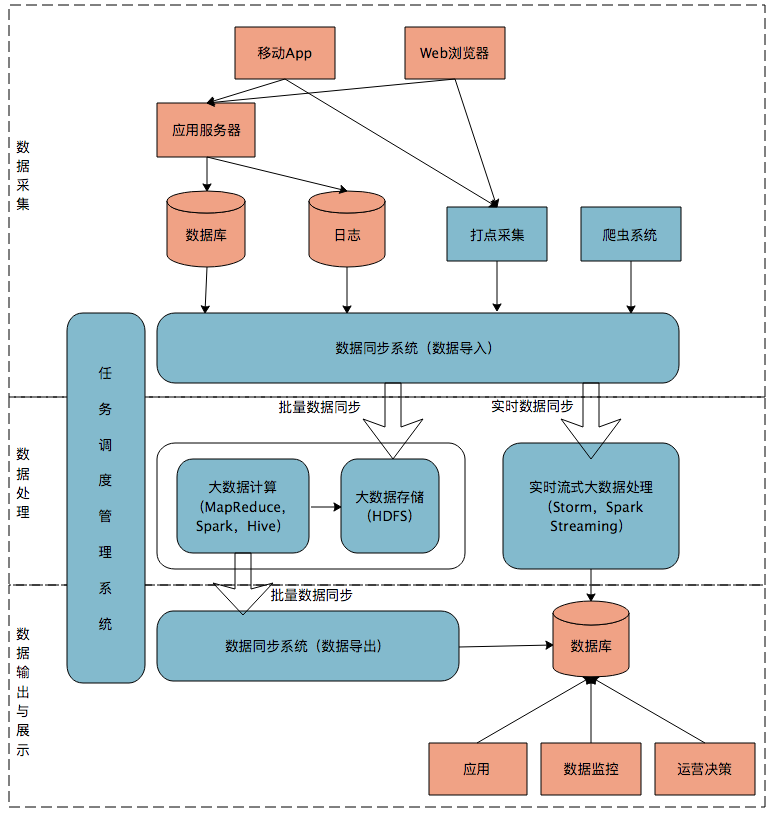
\includegraphics[width=0.50\paperwidth]{img/introduction/big-data-framework.png}
	\caption{典型的互联网大数据平台架构。}
	\label{fig:frame}
	%\vspace{-.15in}
\end{figure}

% \subsection{内存缓存}
% \par 在大数据平台中(图~\ref{fig:frame}),数据处理是非常重要的一环,实现对数据的高效清洗、存储和挖掘是这个环节的目标。对计算能力的需求随着数据量的急剧增加而增加,但是单机的处理能力和 I/O 性能并没有跟上这种增长,越来越多的企业不得不向外扩展他们的计算至集群模式\cite{Zaharia:2016:AFG:3002856}。集群环境对编程平台提出了更高的要求,主要有三方面,一是程序需要并行化执行,二是需要强大的容错能力,三是动态地扩展和缩减计算资源,为此,越来越多的编程模型被设计出来。在存储方面,谷歌提出了分布式文件系统GFS(Google File System)\cite{51},对应的开源实现是HDFS(Hadoop File System)\cite{hdfs},它实现了对成千上万台机器上的大规模数据进行高效地存储、访问,并且具有高度容错能力。计算框架方面,起初,谷歌的 MapReduce\cite{dean2008mapreduce}提出了一种简单通用而且能够自动处理故障的批处理计算模型,但是它将中间以及最终结果保存在磁盘上,消耗大量I/O时间,不利于重用计算结果。Spark\cite{Zaharia:2016:AFG:3002856}、Pregel\cite{malewicz2010pregel}等采用内存计算方案来加速计算,实现数据的重复利用。很多系统的性能瓶颈主要是I/O,包括磁盘读写和网络远程读写的延迟,为了进一步提高性能,一种典型的方法是部署缓存,并且将数据在分布式集群中服务器的内存进行缓存\cite{ananthanarayanan2012pacman},并且尽力实现计算任务和数据的本地性(locality)。内存的读写速度远高于磁盘,将计算与数据部署在相同的机器也能节约网络开销。
\par 在大数据平台中(图~\ref{fig:frame}),数据处理是非常重要的一环,实现对数据的高效清洗、存储和挖掘是这个环节的目标。对计算能力的需求随着数据量的急剧增加而增加,但是单机的处理能力和 I/O 性能并没有跟上这种增长,越来越多的企业不得不向外扩展他们的计算至集群模式\cite{Zaharia:2016:AFG:3002856}。集群环境对编程平台提出了更高的要求,主要有三方面,一是程序需要并行化执行,二是需要强大的容错能力,三是动态地扩展和缩减计算资源,为此,越来越多的编程模型被设计出来。在存储方面,谷歌提出了分布式文件系统GFS(Google File System)\cite{51},对应的开源实现是HDFS(Hadoop File System)\cite{hdfs},它实现了对成千上万台机器上的大规模数据进行高效地存储、访问,并且具有高度容错能力。计算框架方面,起初,谷歌的 MapReduce\cite{dean2008mapreduce}提出了一种简单通用而且能够自动处理故障的批处理计算模型,但是它将中间以及最终结果保存在磁盘上,消耗大量I/O时间,不利于重用计算结果。Spark\cite{Zaharia:2016:AFG:3002856}、Pregel\cite{malewicz2010pregel}等采用内存计算方案来加速计算,实现数据的重复利用。

\subsection{集群缓存}
\par 由于近来数据中心架构的改进~\cite{singh2015jupiter} 和高速网络设备的出现\cite{huawei_nuwa,asanovic2014firebox,alistarh15a},网络带宽和存储器I/O带宽之间的差距正在迅速减小~\cite{latency_trends,p802_3ba,Han13a,Gao16a},因此,云计算系统的性能瓶颈正迅速从网络转变为存储器I/O。先前的工作证明从本地硬盘读取数据相比网络远程读取并没有显著的优势 ~\cite{Ananthanarayanan11a},这个结论同样适用于固态硬盘(SSD)。最近的一个研究~\cite{Jonas17a} 表明将数据存储在EC2实例的一个本地SSD上甚至比把数据写到Amazon S3 ~\cite{amazons3}上还要慢,Amazon S3是一个远程的提供了PUT/GET接口的对象存储服务。当磁盘本地化变得无关紧要,云端对象存储如 Amazon S3~\cite{amazons3}、 Windows Azure Storage~\cite{azure_storage}、和OpenStack Swift~\cite{swift}等,逐渐取代与计算同地的存储(尤其是HDFS~\cite{shvachko2010hadoop}),作为数据密集型应用的首选存储方式。

\par 然而,云端对象存储在磁盘I/O上依然是瓶颈~\cite{rashmi2016ec},因为从磁盘读数据比从内存读数据慢至少两个数量级,考虑到这个问题,集群缓存系统,例如Alluxio~\cite{alluxio}、Memcached~\cite{memcached}和Redis~\cite{redis},被越来越多的云端对象存储系统部署来提供内存速度级别的低延迟数据访问,而集群缓存系统面对的一个很大的挑战便是如何实现负载均衡。

\par 一个能够实现分布式内存缓存的系统是Alluxio。Alluxio\cite{li2014tachyon}是开源的分布式内存文件系统,旨在作为上层繁多的计算框架(如MapReduce、Apache Spark、Apache Storm、Apche Mahout等)与底层存储层(如文件系统、对象存储、键值对存储等)的中间层,提供统一的文件读写的接口,实现全局的数据访问、高效的内存数据共享、跨应用的数据管理、高效的网络带宽利用,它借助“血缘关系”、检查点机制提供强大的容错能力。鉴于这些特点,alluxio也非常适合作为内存缓存系统,进一步加速数据分析应用。


\subsection{负载均衡}
\par 上一小节提及的Apache Spark等内存计算方案的一个重要挑战是负载不均,在先前工作 
\cite{ananthanarayanan2011scarlett,rashmi2016ec} 中,研究人员已经发现了生产集群中负载不均的两个来源:\emph{文件热门程度差别} 和 \emph{网络流量不均}。

\par 在数据中心中,我们普遍观察到,文件(数据对象)热门程度差别极大,并且遵循Zipf分布~\cite{rashmi2016ec, ananthanarayanan2011scarlett, ananthanarayanan2012pacman, li2014tachyon},也就是说,数据访问的大部分请求是由一小部分非常热门的文件贡献的。图~\ref{fig:Yahoo_trace}描述了Yahoo!集群查询数据集~\cite{yahoo!_trace}中文件的热门程度和文件大小的分布,从这个数据集可以得到某两个月内对超过四千万个文件的访问的统计数据。我们发现绝大多数文件($\sim 78\%$)存储的是冷门数据,很少被访问($<10$ times),只有 $2\%$ 的文件有高访问量($\ge100$),这些文件通常比那些冷门的文件大很多($15$-$30 \times$)。由于这些文件较大的体积和较高的访问量,缓存这些文件的服务器很容易负荷过重。

\begin{figure}[t]
\centering
   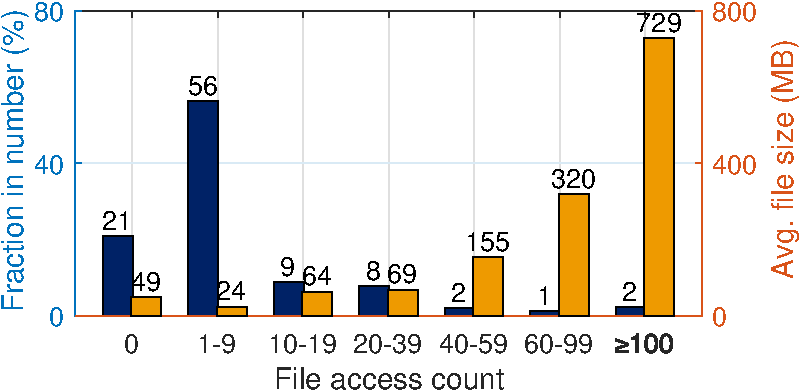
\includegraphics[width=0.5\textwidth]{img/introduction/Yahoo_pop-eps-converted-to.pdf}
   \caption{Yahoo!集群上观察到的文件热门程度(蓝色)和文件大小(橙色)的分布~\cite{yahoo!_trace}.}
\label{fig:Yahoo_trace}
\vspace{-.1in}
\end{figure}

\par 这个问题由于网络负载不均而加重,这在生产环境的数据中心非常普遍~\cite{Kandula09a,Chowdhury13a,Greenberg09a,rashmi2016ec},例如,在研究~\cite{rashmi2016ec}中,研究者测量了Facebook一个集群所有上行和下行链路中最大利用率和平均利用率的比值,结果表明这个比值在半数以上的时间里保持在4.5以上,这意味着严重的负载不均。在SP-Cache~\cite{Yu:2018:SLR:3291656.3291658}的研究中,研究人员分别测量了在有无内存缓存的情况下,不同请求速率下的文件的平均读延迟,结果表明~\ref{fig:impact_of_imbalance}当集群负载不重时(每秒$5$个请求),内存缓存带来了显著性好处,降低平均读延迟达 $5\times$,然而,当负载骤然增大,集群中的热点机器变得突出,缓存带来的好处迅速减少,尤其当请求速率大于$9$,读延迟就由热点服务器的网络拥塞决定,内存缓存就变得\emph{无关紧要}。

\begin{figure}[t]
    \centering
    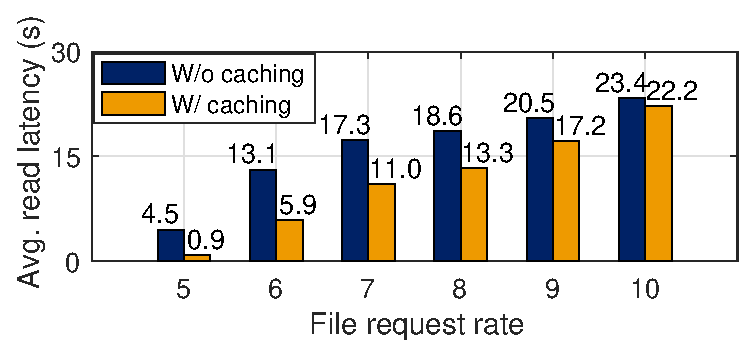
\includegraphics[width=0.8\textwidth]{img/introduction/latencies_under_imbalance}
    \caption{有/无缓存的情况下平均读延迟随着负载增加而增加。}
    \label{fig:impact_of_imbalance}
    \vspace{-.15in}
\end{figure}

\section{研究现状}

\par 当今的数据并行集群依赖内存计算方案来进行高性能的数据分析工作\cite{li2014tachyon, presto, Zaharia:2016:AFG:3002856, power2010piccolo, memcached, memsql},通过将数据对象缓存在内存中, I/O 密集型应用相对于传统的磁盘解决方案能够获得数量级的性能提升\cite{li2014tachyon, Zaharia:2016:AFG:3002856, power2010piccolo}

\par 然而,内存计算方案面对的一个严峻的挑战是缓存服务器之间严重的负载不均衡。在生产集群中,数据对象有严重的热门程度差别,这意味着对一小部分非常热门的文件访问占据了总访问的很大一部分\cite{rashmi2016ec, ananthanarayanan2011scarlett, ananthanarayanan2012pacman}。存储有热门文件的缓存服务器因此变为访问热点,这个问题因为网络的负载不均衡而进一步恶化。据报道,在 Facebook 的一个集群中,负载最重的链路的利用率在 $50\%$ 的时间里比 平均链路利用率高出 4.5 倍\cite{rashmi2016ec}。访问热点和网络负载不均导致了 I/O 性能极大下降,这甚至可能会抵消内存计算带来的性能提升。

\par 因此,保证负载均衡是提高集群缓存性能的关键,这方面的解决方案包括选择性复制\cite{ananthanarayanan2011scarlett}、纠删码\cite{rashmi2016ec}和选择分割\cite{Yu:2018:SLR:3291656.3291658},前二者是借助缓存冗余来减缓访问热点机器的负担,第三个是根据文件的热门程度将文件分割成不同份数,并随机放置在不同服务器上,分散请求负载。

\subsection{选择复制}

\par 选择复制方案基于文件的热门程度对文件进行复制~\cite{ananthanarayanan2011scarlett,hong2013understanding},也就是说,一个文件的访问频率越高,它会越多被复制,并分散在集群中,一个文件的读请求就能随机选择一台含有这个文件副本的服务器提供服务。这样,读请求的负载就被均匀分散,提高负载均衡。

\par 虽然选择复制已被证明对于基于磁盘的存储系统是有效的~\cite{ananthanarayanan2011scarlett},但是因为复制带来了高额的内存开销,它在集群缓存上表现不佳~\cite{huang2014characterizing,rashmi2016ec}。研究~\cite{Yu:2018:SLR:3291656.3291658}的实验得出,内存开销的 \emph{线性增加}(热门文件副本数增加)换来了读延迟的 \emph{亚线性降低},而且热门文件的体积通常比较大(图~\ref{fig:Yahoo_trace})。

\subsection{纠删码}

\par 有研究利用\emph{纠删码}~\cite{huang2012erasure,sathiamoorthy2013xoring} 来实现缓存服务器之间的负载均衡且避免产生高额的内存开销。一个$(k,n)$的纠删码方案能够将一个文件均匀地切分成$k$份,然后计算同样大小的$n-k$个 \emph{奇偶校验分区},原始文件能通过解码$n$份中的任意$k$份来获得,从而使得读请求的负载被分散到$n$台服务器上。内存的额外开销是$(n-k)/k$,在实际设定中比选择复制低(至少 $1\times$)。
\par 这个方法的一个有效实现是EC-Cache~\cite{rashmi2016ec},它在读取文件时通过\emph{迟绑定}来减轻落后机器的影响,换句话说,EC-Cache随机读取文件分区中的$k+1$份,等待其中的$k$份完成读取,而不是恰好读取$k$份。EC-Cache在读文件的中位和尾延迟都比选择复制低很多~\cite{rashmi2016ec}。然而,EC-Cache在读(写)时带来巨大的解码(编码)的额外开销,即使有高度优化的编码和实现方案,解码的开销仍会对读请求产生高达$30\%$~\cite{rashmi2016ec}延迟。

\subsection{选择分割}

\par 研究~\cite{Yu:2018:SLR:3291656.3291658}中提出了SP-Cache来实现集群缓存的负载均衡,同时避免高额的内存和计算开销。它选择性地将热门文件根据其大小和热门程度,分割成一定数目的文件分区,随机缓存到不同的缓存服务器上,这样分散了读请求的负载,同时读操作可以并行,提升性能。SP-Cache建立了一个上限分析来量化平均延迟~\cite{Yu:2018:SLR:3291656.3291658},并基于这个推导设计了一个高效的算法来决定每个文件的最佳分区数量,文件分割的数目太小则不足以缓解热点机器的压力,分割的数目太大则容易受到慢机器的影响。此外它采集一段时间内集群中文件的访问数据,周期性地调整各个文件的分区数目。选择分割在不产生高额内存和计算开销的情况下实现可负载均衡,但因为其分割的特性,缓存无冗余,容错性依赖底层文件系统,且读取文件必须读取所有分区,会受到慢机器的影响。

\subsection{更细粒度负载均衡}

\par 以上方案都是针对一般意义上的文件来考虑负载均衡的,优点是非常通用,毋需考虑文件的语义,对于任何格式的文件都可以使用。它们负载均衡的粒度是文件,那么问题来了,能否在更细的粒度进行负载均衡,提高缓存效率呢?对于语义清晰的结构化数据,比如Parquet文件~\cite{parquet},如果在文件的内部列与列存在热门程度差异,列之间被共同查询的概率也存在差异,那么就没有必要去分割或者复制整个文件,只要对一个文件热门的这一部分,例如其中一列或者多列进行复制或者分割就行。这样能够节约内存,提高使用效率,因为内存总是有限的,而且一部分内存需要给计算任务使用,那么留作缓存的就更少了。这个目标的挑战在于底层分布式文件系统需要了解文件的语义,与上层的应用通信来获得这部分信息,可能产生一定程度的耦合,同时我们需要明智地决定对文件的哪些列进行复制或分割,在哪些机器上进行缓存。

\section{研究的目的与内容}
当前的大数据系统主要采用复制的方式来进行容错和负载均衡,而服务器内存的容量往往有限,缓存会产生不可忽视的内存开销。根据本项目的前期调研,生产集群中结构化数据(数据表)的不同列之间,热门程度(被访问热度)存在差异,列与列之间共同被查询的概率也存在差异,我们希望复制数据表中比较热门的列,而不是全表,并基于列与列之间被共同查询的概率设计一定的放置策略,实现以更少的内存,来获得相似的负载均衡效果的目标,从而节约资源,提高缓存效率。

总的来说,本课题的主要研究内容是上文提出的针对结构化数据文件的更细粒度(列级别)的负载均衡方案,具体来说:

\begin{itemize}
	\item 利用具有代表性的基准查询数据集,如TPC-DS, TPC-H等,测量数据表中列之间的查询频率,以及列与列之间被共同查询的频率,分析其中的统计及其他客观规律,为本项目的可行性奠定理论基础。
	\item 通过实验探究SQL查询过程中,数据的shuffle过程对任务执行时间的影响,证明数据表中相关列“捆绑放置”(bundle)的有效性,进一步强化项目的理论基础。
	\item 搭建Spark SQL~\cite{armbrust2015spark},Alluxio~\cite{alluxio},HDFS~\cite{shvachko2010hadoop}为主的集群系统,探索各组件之间通信协作机制,为项目方案实现奠定基础。
	\item 基于已有条件,主要在Alluxio~\cite{alluxio}基础上添加模块,使得Alluxio能够获取热门度以及关联性等信息,查阅相关文献,设计实现细粒度的负载均衡算法,并在AWS EC2搭建实验环境,进行测试。
\end{itemize}

\section{论文结构}

% \section{数学公式}
% \subsection{简单的数学公式}
% \textbf{卷积}(\textbf{convolution})在图像分析的线性方法中是一种重要的运算。卷积是一个积分,反映一个函数$f(t)$在另一个函数上$h(t)$移动时所重叠的量。函数$f$和$h$在有限域$[0,t]$上的$1D$卷积$f*h$由下式给出:
%  $$(f*h)(t) \equiv \int_0^t {f(\tau )h(t - \tau )d\tau } $$

% \subsection{带自动编号的公式}
% 这里可以限定在$[0,t]$区间,原因是我们假设负坐标部分的值是0。为了准确起见,我们还可以将卷积积分的上限扩展为$( - \infty ,\infty )$:
% \begin{equation}(f*h)(t) \equiv \int_{ - \infty }^\infty  {f(\tau )h(t - \tau )d\tau }  = \int_{ - \infty }^\infty  {f(t - \tau )h(\tau )d\tau }
%   \end{equation} 

% \subsection{带等号对齐的公式}
% 卷积可以推广到更高维。令$2D$函数$f$和$h$的卷积$g$记为$f*h$,则有:
% \begin{equation}
% \begin{aligned}
% (f*h)(x,y) &= \int_{ - \infty }^\infty  {\int_{ - \infty }^\infty  {f(a,b)h(x - a,y - b)} } dadb\\
%  &= \int_{ - \infty }^\infty  {\int_{ - \infty }^\infty  {f(x - a,y - b)h(a,b)} } dadb\\
% \end{aligned}
% \end{equation}

% \section{伪代码}
% 在写论文的时候我们通常要写伪代码,伪代码里面有时甚至还要包含数学公式(如根号一类的)。伪代码会自动找一个比较好的位置插入图片。

% \begin{algorithm}
%     \caption{用归并排序求逆序数}
%     \begin{algorithmic}[1] %每行显示行号
%         \Require $Array$数组,$n$数组大小
%         \Ensure 逆序数
%         \Function {MergerSort}{$Array, left, right$}
%             \State $result \gets 0$
%             \If {$left < right$}
%                 \State $middle \gets (left + right) / 2$
%                 \State $result \gets result +$ \Call{MergerSort}{$Array, left, middle$}
%                 \State $result \gets result +$ \Call{MergerSort}{$Array, middle, right$}
%                 \State $result \gets result +$ \Call{Merger}{$Array,left,middle,right$}
%             \EndIf
%             \State \Return{$result$}
%         \EndFunction
%         \State
%         \Function{Merger}{$Array, left, middle, right$}
%             \State $i\gets left$
%             \State $j\gets middle$
%             \State $k\gets 0$
%             \State $result \gets 0$
%             \While{$i<middle$ \textbf{and} $j<right$}
%                 \If{$Array[i]<Array[j]$}
%                     \State $B[k++]\gets Array[i++]$
%                 \Else
%                     \State $B[k++] \gets Array[j++]$
%                     \State $result \gets result + (middle - i)$
%                 \EndIf
%             \EndWhile
%             \While{$i<middle$}
%                 \State $B[k++] \gets Array[i++]$
%             \EndWhile
%             \While{$j<right$}
%                 \State $B[k++] \gets Array[j++]$
%             \EndWhile
%             \For{$i = 0 \to k-1$}
%                 \State $Array[left + i] \gets B[i]$
%             \EndFor
%             \State \Return{$result$}
%         \EndFunction
%     \end{algorithmic}
% \end{algorithm}

% \section{插入图片}
% 在使用该命令的时候,图片会自动找一个他觉得比较好的位置插入图片,我们就不需要担心前面改了文字之后后面的格式乱掉。
% \begin{figure}[htbp!]
% \centering 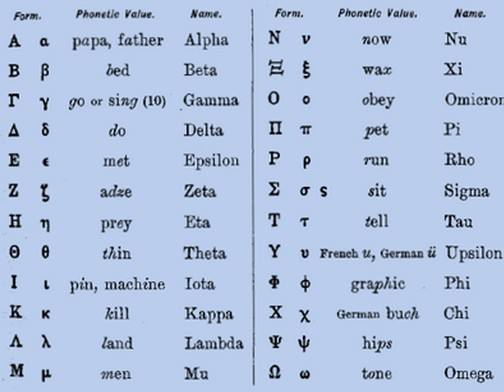
\includegraphics[width=0.9\textwidth]{img/test.jpg} \caption{图片的一个简单应用场景}
% \end{figure}

% \begin{figure}
% \centering
% \subfigure[the first subfigure]{
% 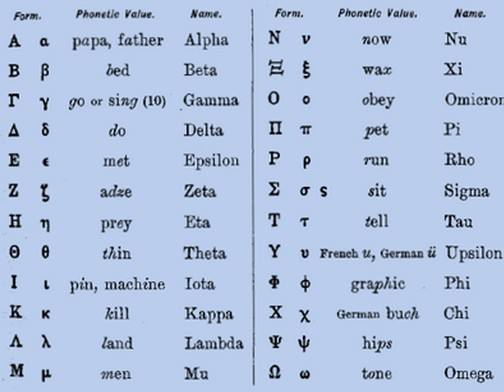
\includegraphics[width=0.4\textwidth]{img/test.jpg} 
% }
% \subfigure[the second subfigure]{
% 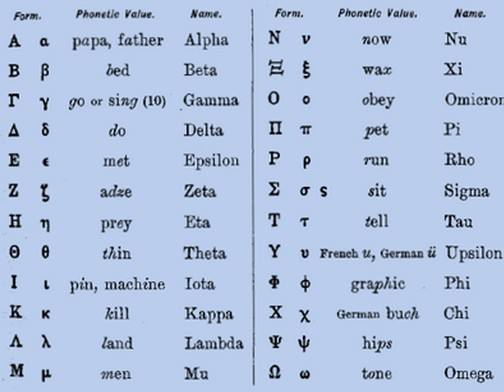
\includegraphics[width=0.4\textwidth]{img/test.jpg} 
% }
% \caption{子图应用场景}
% \end{figure}

% \section{引用论文}
% 使得论文符合要求\cite{ananthanarayanan2011scarlett}\cite{parquet}\cite{p802_3ba}。
%# -*- coding: utf-8-unix -*-
%%==================================================
%% motivation.tex for seuthesis Bachelor Thesis
%%==================================================

\chapter{研究动机}
\label{chp:motivation}


\par 过往的很多工作研究了文件的访问热度(skewed file popularities)差别很大的情况下集群缓存系统的负载均衡,在这些工作中,文件复制是被广泛应用的方法。例如,HDFS默认把一份文件复制为3份;当缓存服务器上发生缓存缺失(cache miss),Alluxio弹性增加热门文件在内存中的副本数。

\par 然而文件复制会带来较高的内存开销,最终损害缓存带来的好处。在数据分析的工作中,批处理任务分析结构化数据的情况比较多,结构化数据相比一般意义上的文件具有更多的上下文信息,其中列式存储的文件格式,比如Parquet\cite{parquet},得到越来越多的应用,因为在数据分析的大部分任务中,通常需要按列进行读取,而不是按行读取,并且列式存储把相同类型的数据归在一起,压缩比可以很高。那么问题来了,针对采用列式存储的结构化数据,我们是否能够根据其特有的性质,保证负载均衡的效果的同时,降低文件复制的开销呢?以往的研究工作表明,对一小部分热门文件(被高频访问的文件)访问占据了集群总访问量的大部分,我们猜想,那么对于结构化数据来说,例如具体一张数据表,列与列之间是否存在热门程度的差异呢?如果猜想成立,直观上来说,对于一张表,我们可以只复制最热门的几列,就能达到接近复制全表的负载均衡效果,同时能够降低缓存开销。

\par 如果按照上文所述,仅复制最热门的若干列,缓存在不同的机器上,那么在执行分布式SQL任务的时候,极有可能发生表内部的数据shuffle,我们需要探究shuffle对任务执行时间的影响。直观上来说,数据shuffle带来网络通信上的开销,会降低任务执行的效率,那么在考虑被复制的列在集群里的放置策略时,我们也需要考虑列与列之间被共同访问的概率,如果两列有很大可能性会被一起访问,那么可以考虑将它们“捆绑”(bundle)在一起放置。

\par 在本章~\ref{sec:col-access}节中,我们通过对标准基准数据集TPC系列的分析,来证明数据表中列与列之间,被访问频率存在差异,并且当考虑两两之间被共同访问的概率,两列各自的被访问频率越高,它们被共同访问的频率也越高。在~\ref{sec:data-shuffle}节中,我们通过实验证明数据shuffle会对SQL任务的执行会显著降低任务的执行效率。

\section{列的访问规律}
\label{sec:col-access}

\par 首先我们研究了具有代表性的基准标准测试程序TPC系列中的TPC-H,TPC-DS,TPC-xBB的各个数据表中的列的访问规律。

\subsection{实验设置}

\par 我们通过2.4.0版本的Spark SQL执行三种标准测试程序提供的查询任务。对于每一种,我们生成1 GB\footnote{这个实验与数据量无关,因为数据表的个数和每个表的访问规律不回随着表的规模而改变}的数据,数据存储为Parquet格式,然后将查询任务依次提交。三种标准测试程序各自包含的数据表的数量和查询任务的数量总结在表格~\ref{tab:setup}中。当执行查询任务的时候,我们记录对列的访问数据,以此来分析列级别的数据访问的性质。我们从结果中观察到以下两个现象。

\begin{figure}[t]
	\centering
	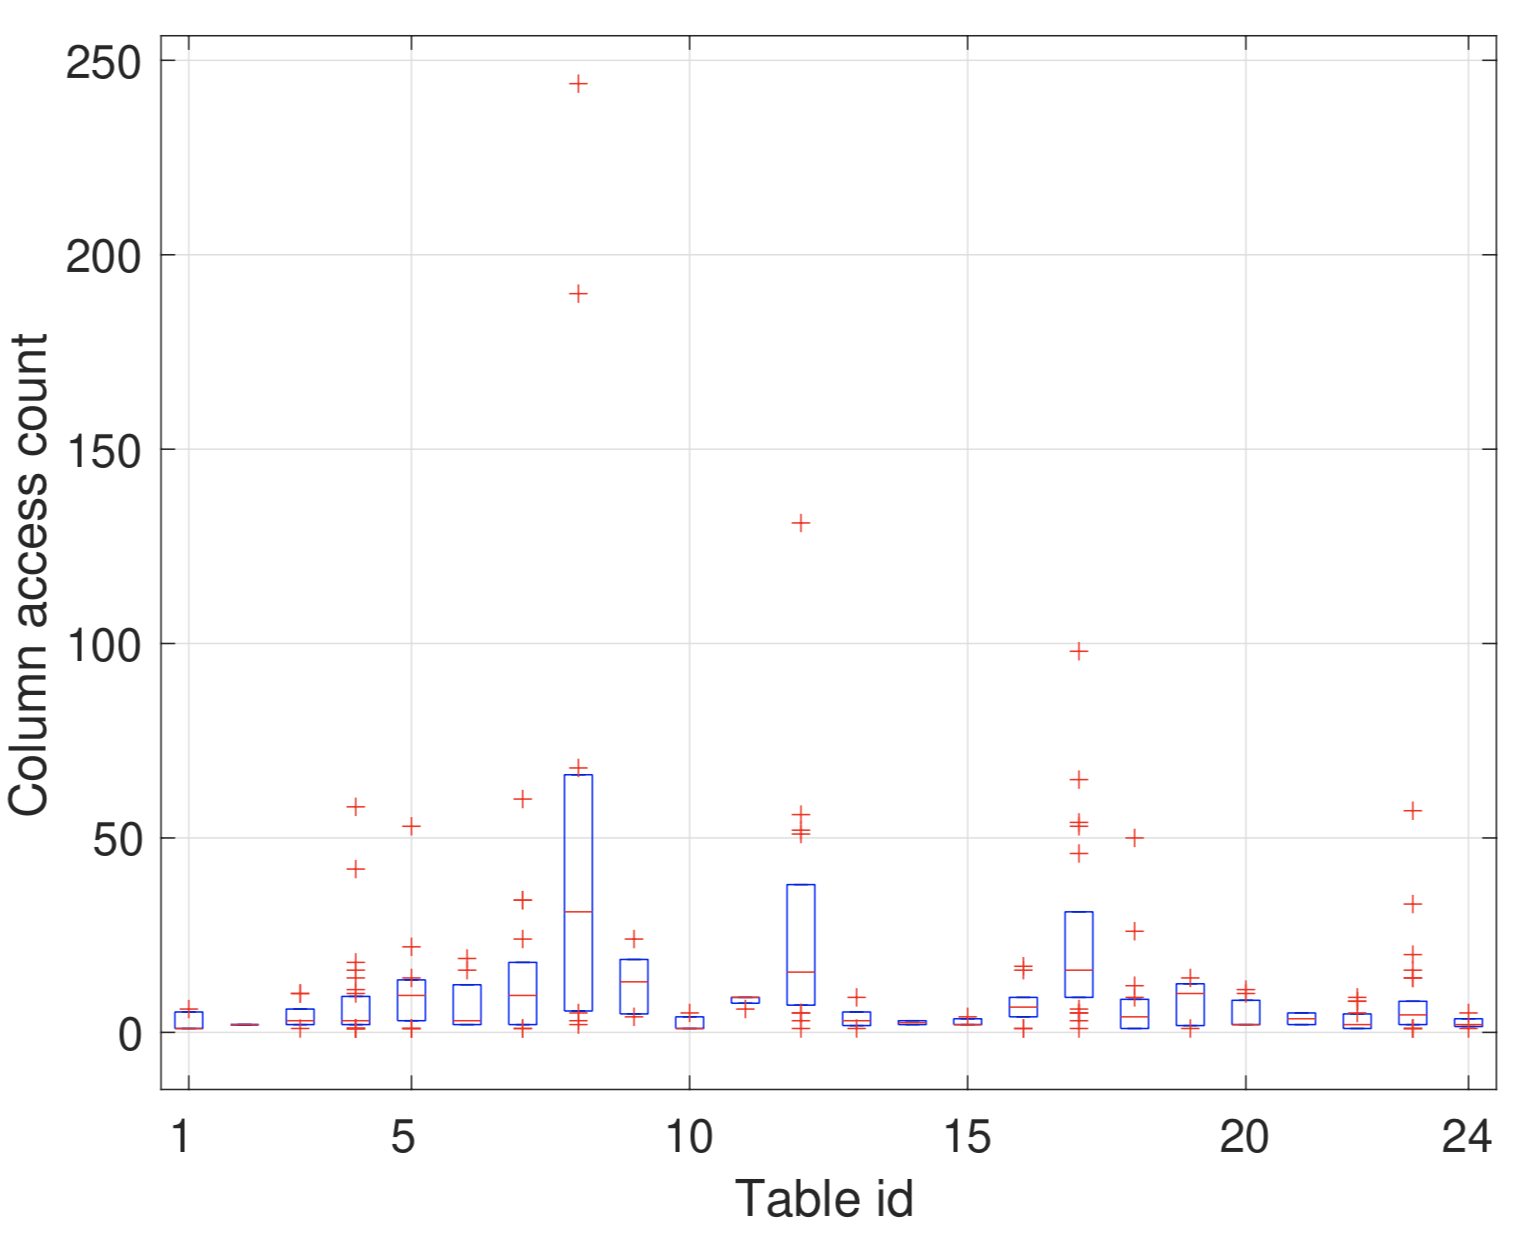
\includegraphics[width=0.5\textwidth]{img/motivation/column-pop}
	\caption{TPC-DS标准测试程序中所有数据表的列访问计数的分布。箱形图展示了每张数据表里$25$\textsuperscript{th}分位,中位数和$75$\textsuperscript{th}分位的列访问次数计数。红色标记表示离群值。}
	\label{fig:tpc-ds-column-pop}
	%\vspace{-.1in}
\end{figure}

\subsection{文件内列访问频率偏差}

\par 在上述三种标准测试程序中,我们观察到,每张数据表内,列的访问频率存在显著差异,即每张表里只有一小部分列被经常访问,而其他的列访问频次比较低。为证明这点,我们对三种标准测试程序中各数据表的列的访问进行了计数。图~\ref{fig:tpc-ds-column-pop}展示了TPC-DS标准测试程序中每张表中列访问计数的分布,箱形图展示了每张数据表里$25$\textsuperscript{th}分位,中位数和$75$\textsuperscript{th}分位的列访问次数计数。每个红色标记表示异常值,特别地,在箱形图上方的红色标记代表该表中访问频率特别高的列。从图上可以看出,对于TPC-DS的多数表,箱形图上方的红色标记远远高于箱形图顶部,这些“热门”的列被访问的次数远远超过均值,这说明文件内列访问频率存在显著偏差。此外,对于各个表而言,表越“热门”(它的列整体上访问频率高),列之间访问频率的差异越大。

\begin{table}[tbp]
    \centering
    \caption{三种标准测试程序的数据}
      \begin{tabularx}{.7\textwidth}{|l|X|X|X|r|}
      \hline
      \textbf{标准测试程序} & \textbf{表的数量} & \textbf{查询任务的数量}  \bigstrut\\ %
      \hline
      TPC-DS & 24  & 99 \bigstrut\\ %
      \hline
      TPC-H & 8  & 22 \bigstrut\\ %
      \hline
      TPC-xBB & 19  & 30 \bigstrut\\ %
      \hline
      \end{tabularx}%
      %\end{tabularx}
    \label{tab:setup}
\end{table}


\par 相似的性质也能在另外两种标准测试程序中看到,图~\ref{fig:count-cdf}展示了三种基准测试程序中所有列的访问计数的总体分布。我们发现,多数的列是“冷门的”,有很多列的访问次数是1,甚至是0,这在TPC-DS(图~\ref{fig:ds-count-cdf})和TPC-xBB(图~\ref{fig:bb-count-cdf})中表现比较明显,而一小部分列有非常高的访问计数。例如,在TPC-DS中,最“热门”的列被访问了多达$89$次。


\begin{figure}[]
    \centering
    \begin{subfigure}[t]{0.5\textwidth}
        \centering
        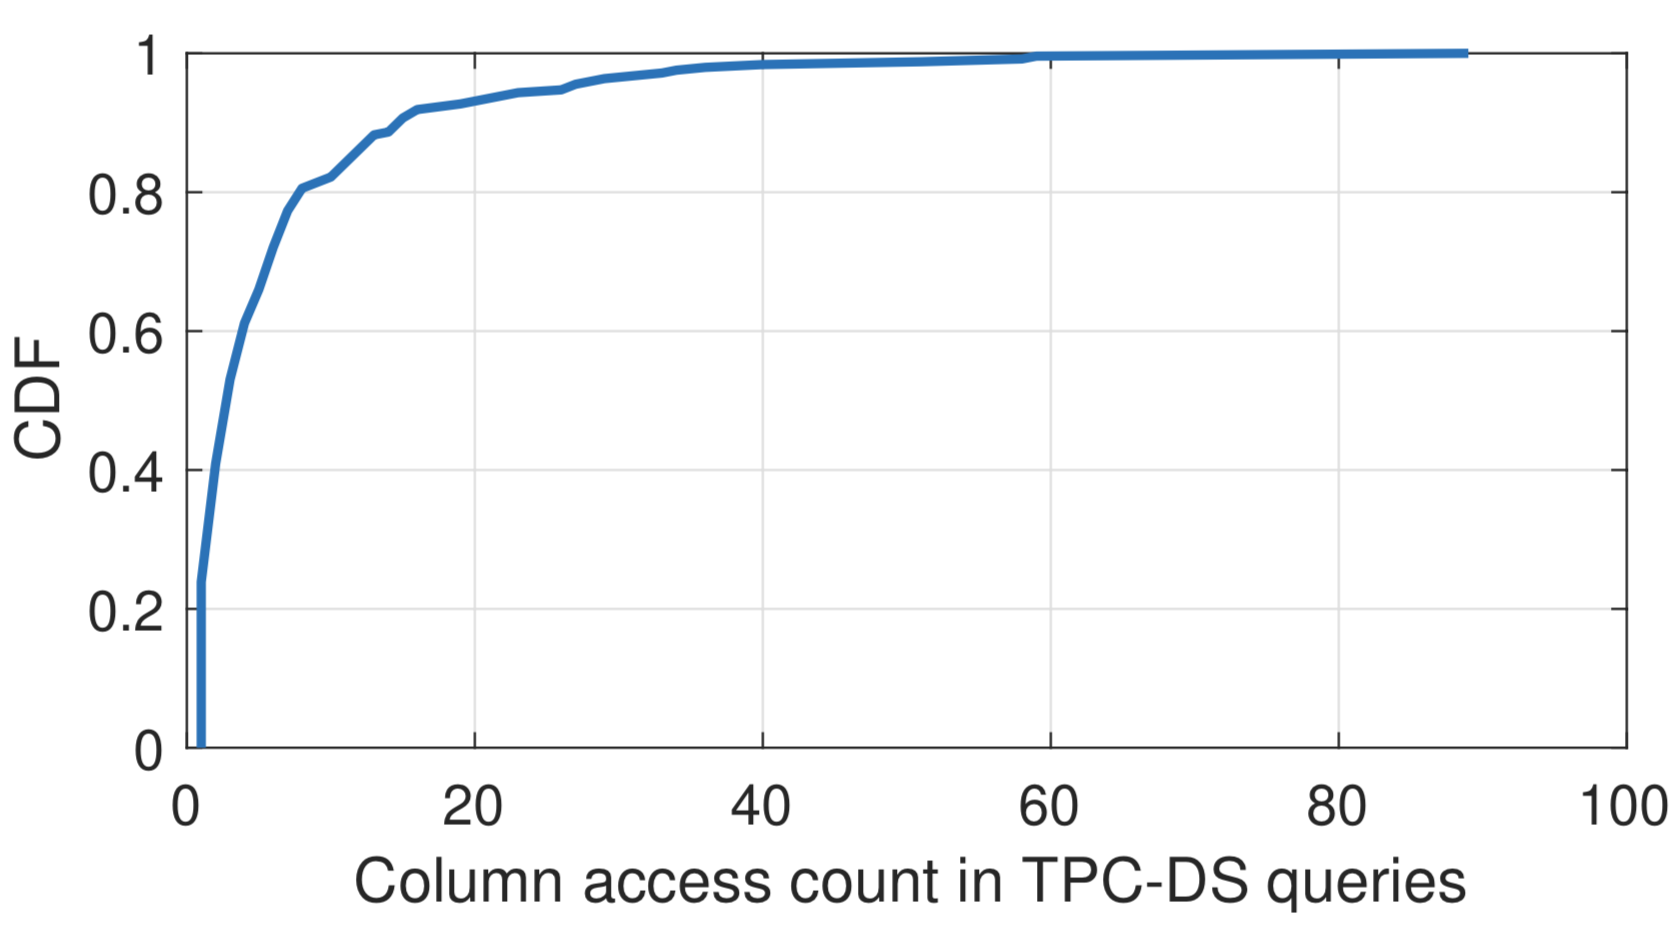
\includegraphics[width=1\textwidth]{img/motivation/ds-count-cdf}
        \caption{TDC-DS.}
        \label{fig:ds-count-cdf}
    \end{subfigure}%

    \begin{subfigure}[t]{0.5\textwidth}
        \centering
        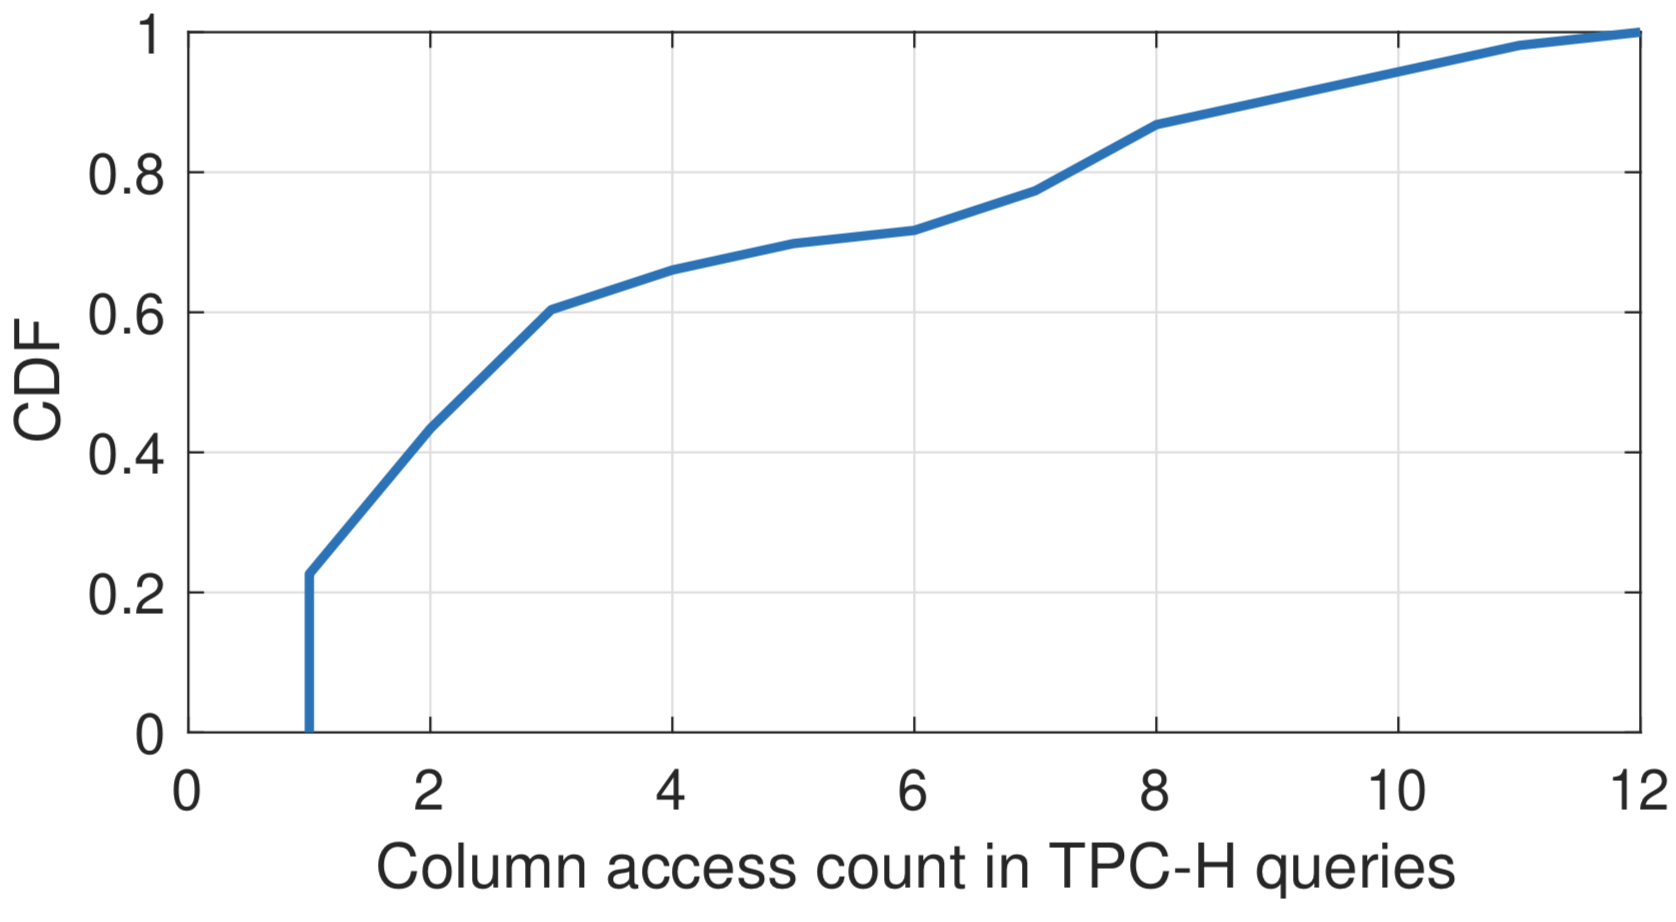
\includegraphics[width=1\textwidth]{img/motivation/h-count-cdf}
        \caption{TDC-H.}
        \label{fig:h-count-cdf}
    \end{subfigure}%

    \begin{subfigure}[t]{0.5\textwidth}
        \centering
        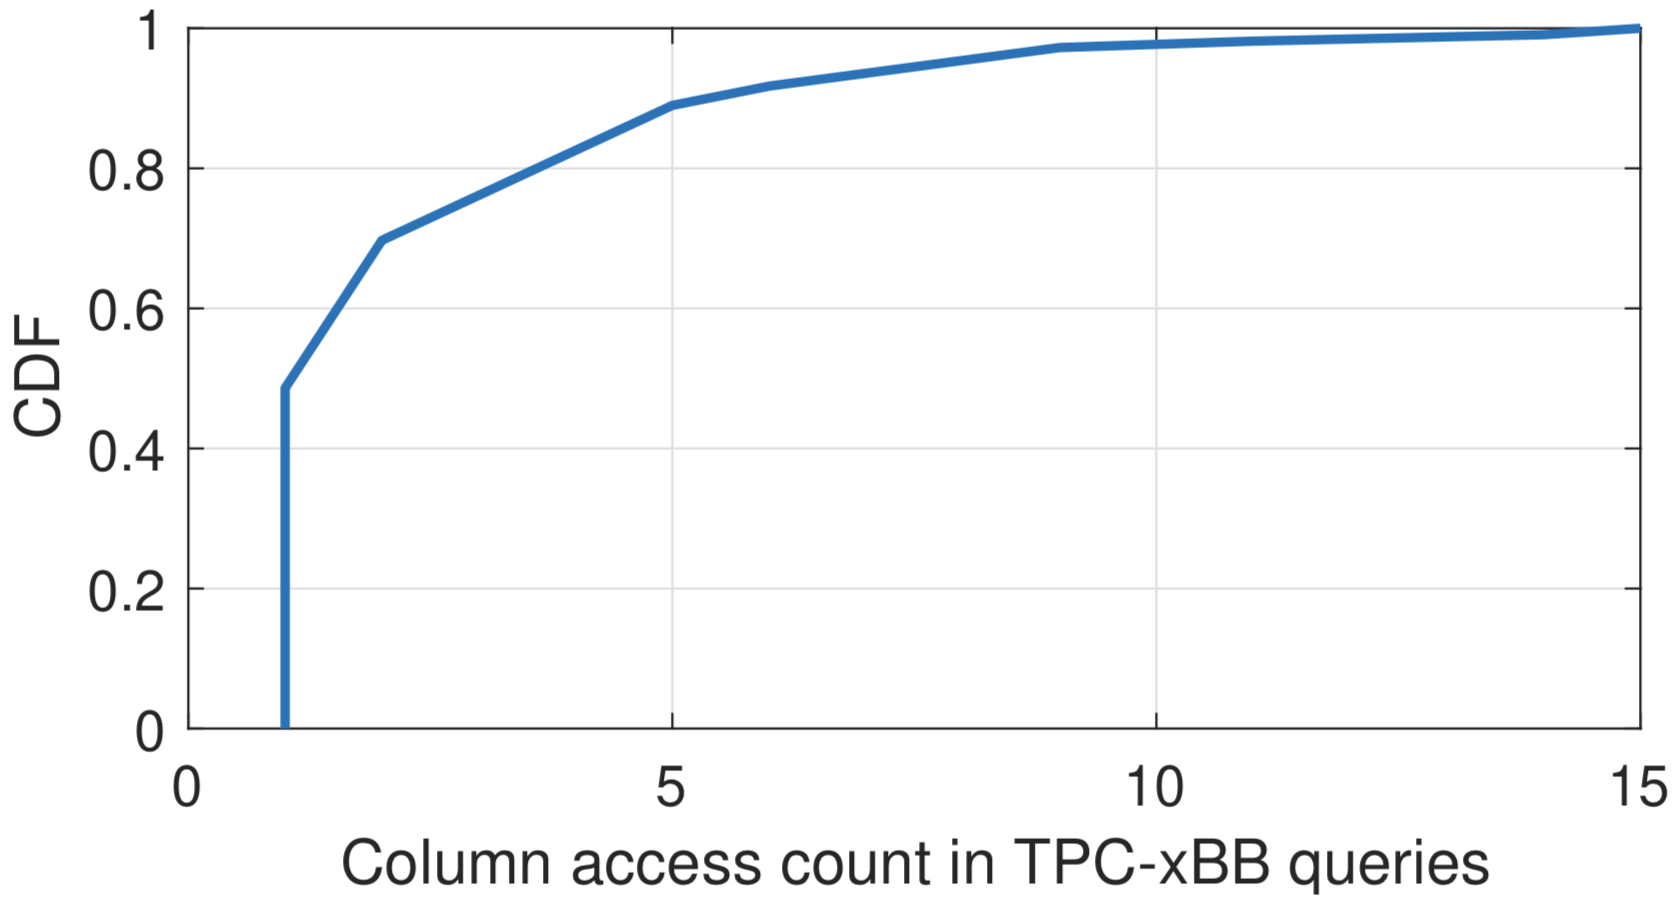
\includegraphics[width=1\textwidth]{img/motivation/xbb-count-cdf}
        \caption{TDC-xBB.}
        \label{fig:bb-count-cdf}
    \end{subfigure}%
    \caption{三种标准测试程序中列访问计数的CDF。}
    \label{fig:count-cdf}
    %\vspace{-.1in}
\end{figure}


\subsection{热门的列被共同访问的规律}
我们观察到的另一个现象是在SQL查询中,“热门”的列有很大概率会被共同访问。为了展示这一点,我们按照列的“热门程度”(访问频次)对列进行排序,绘制访问热图。我们从三个标准测试程序中各选出了一张具有代表性的表,并把结果展示在图~\ref{fig:heatmap}中。在热图里,格 $(i,i)$ (也就是对角线上的格子)代表第$i^{th}$热门的列的访问计数,格子$(i,j)$表示第$i^{th}$热门和第$j^{th}$热门的列在同一个查询任务中被共同访问的概率。从图中可以看出,每张表中越是热门的列,被共同访问的概率越高。

\begin{figure}[]
    \centering
    \begin{subfigure}[t]{0.5\textwidth}
        \centering
        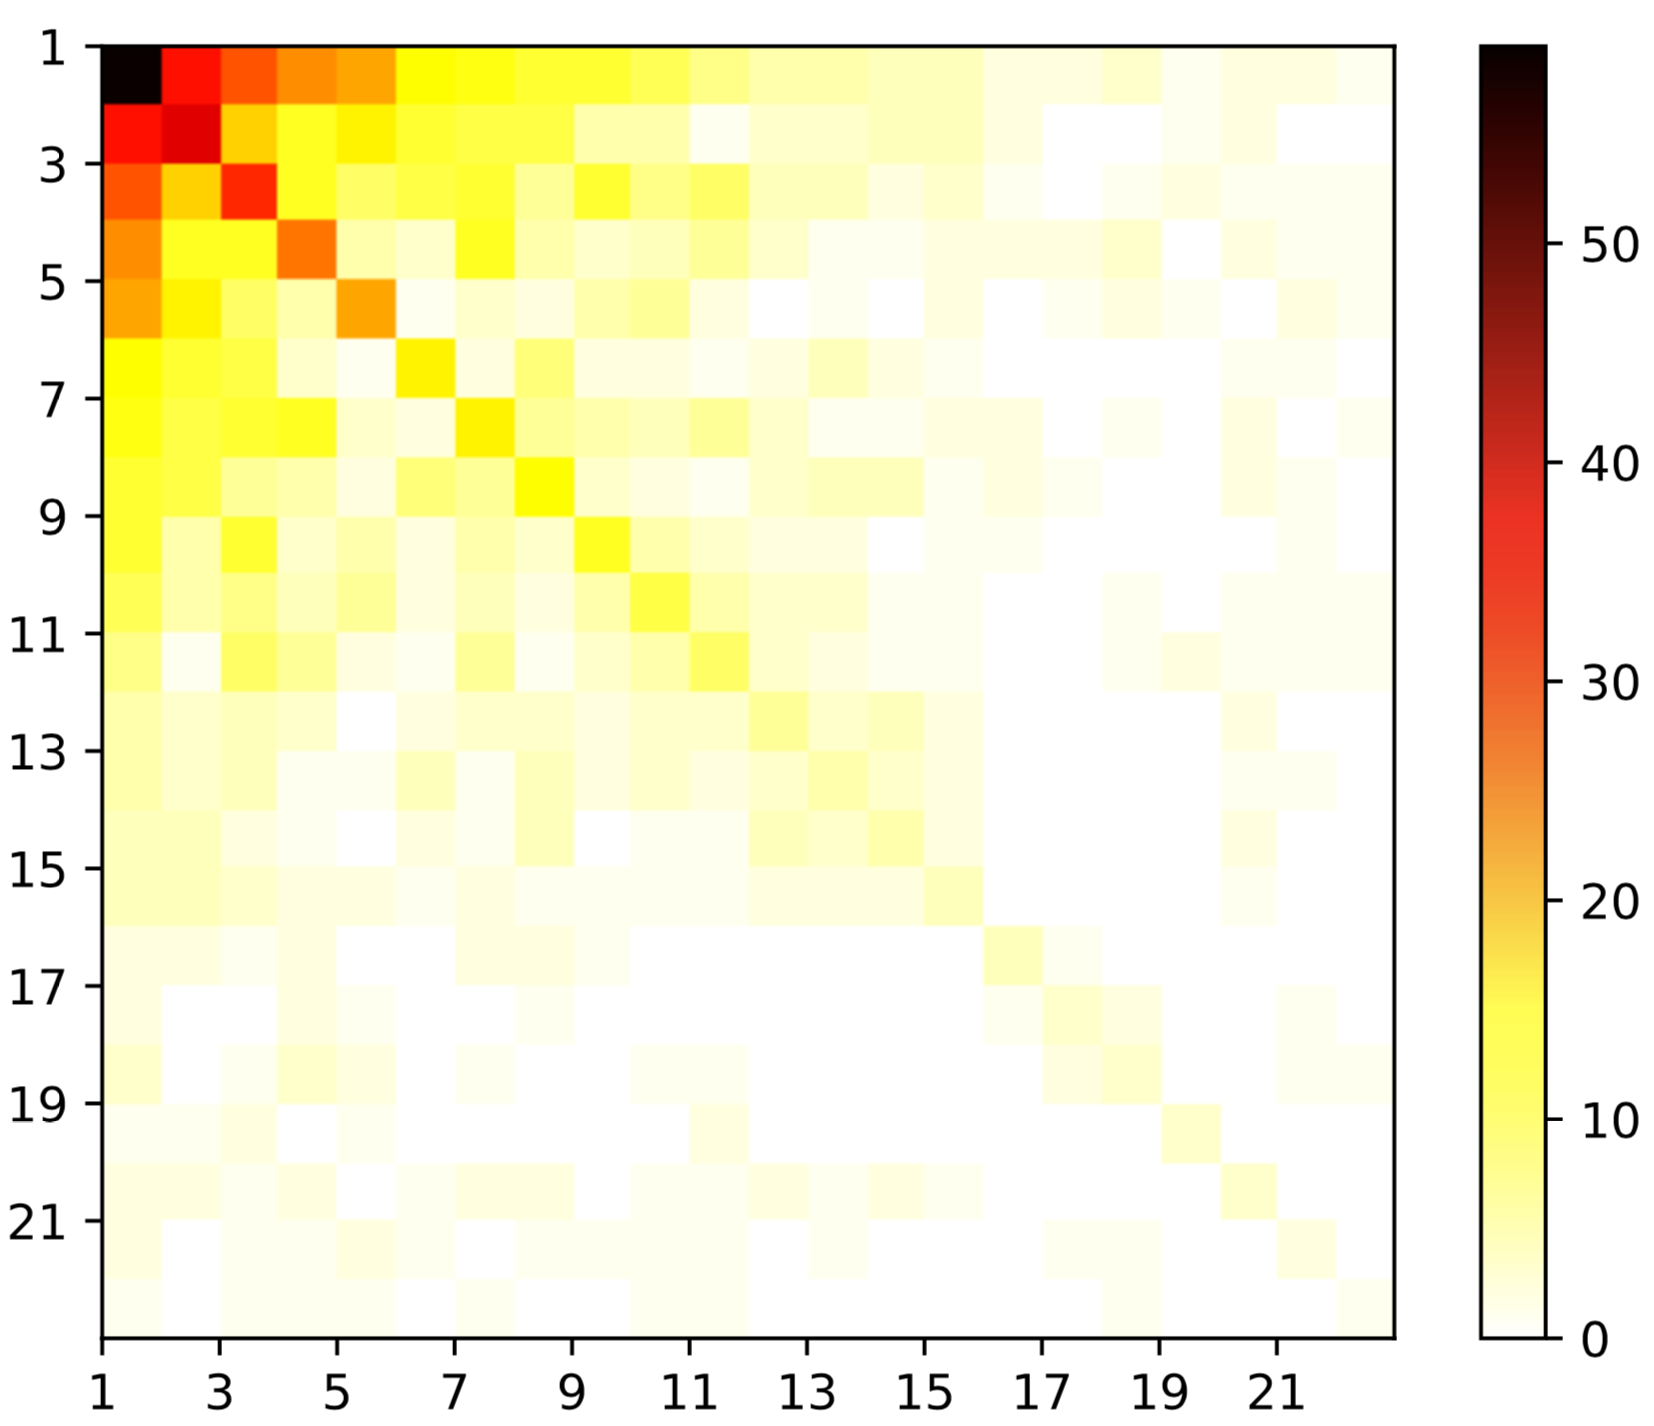
\includegraphics[width=1\textwidth]{img/motivation/tpc-ds-store_sales}
        \caption{TDC-DS中的 $store\_sales$ 表。}
        \label{fig:ds_count_cdf}
    \end{subfigure}%

    \begin{subfigure}[t]{0.5\textwidth}
        \centering
        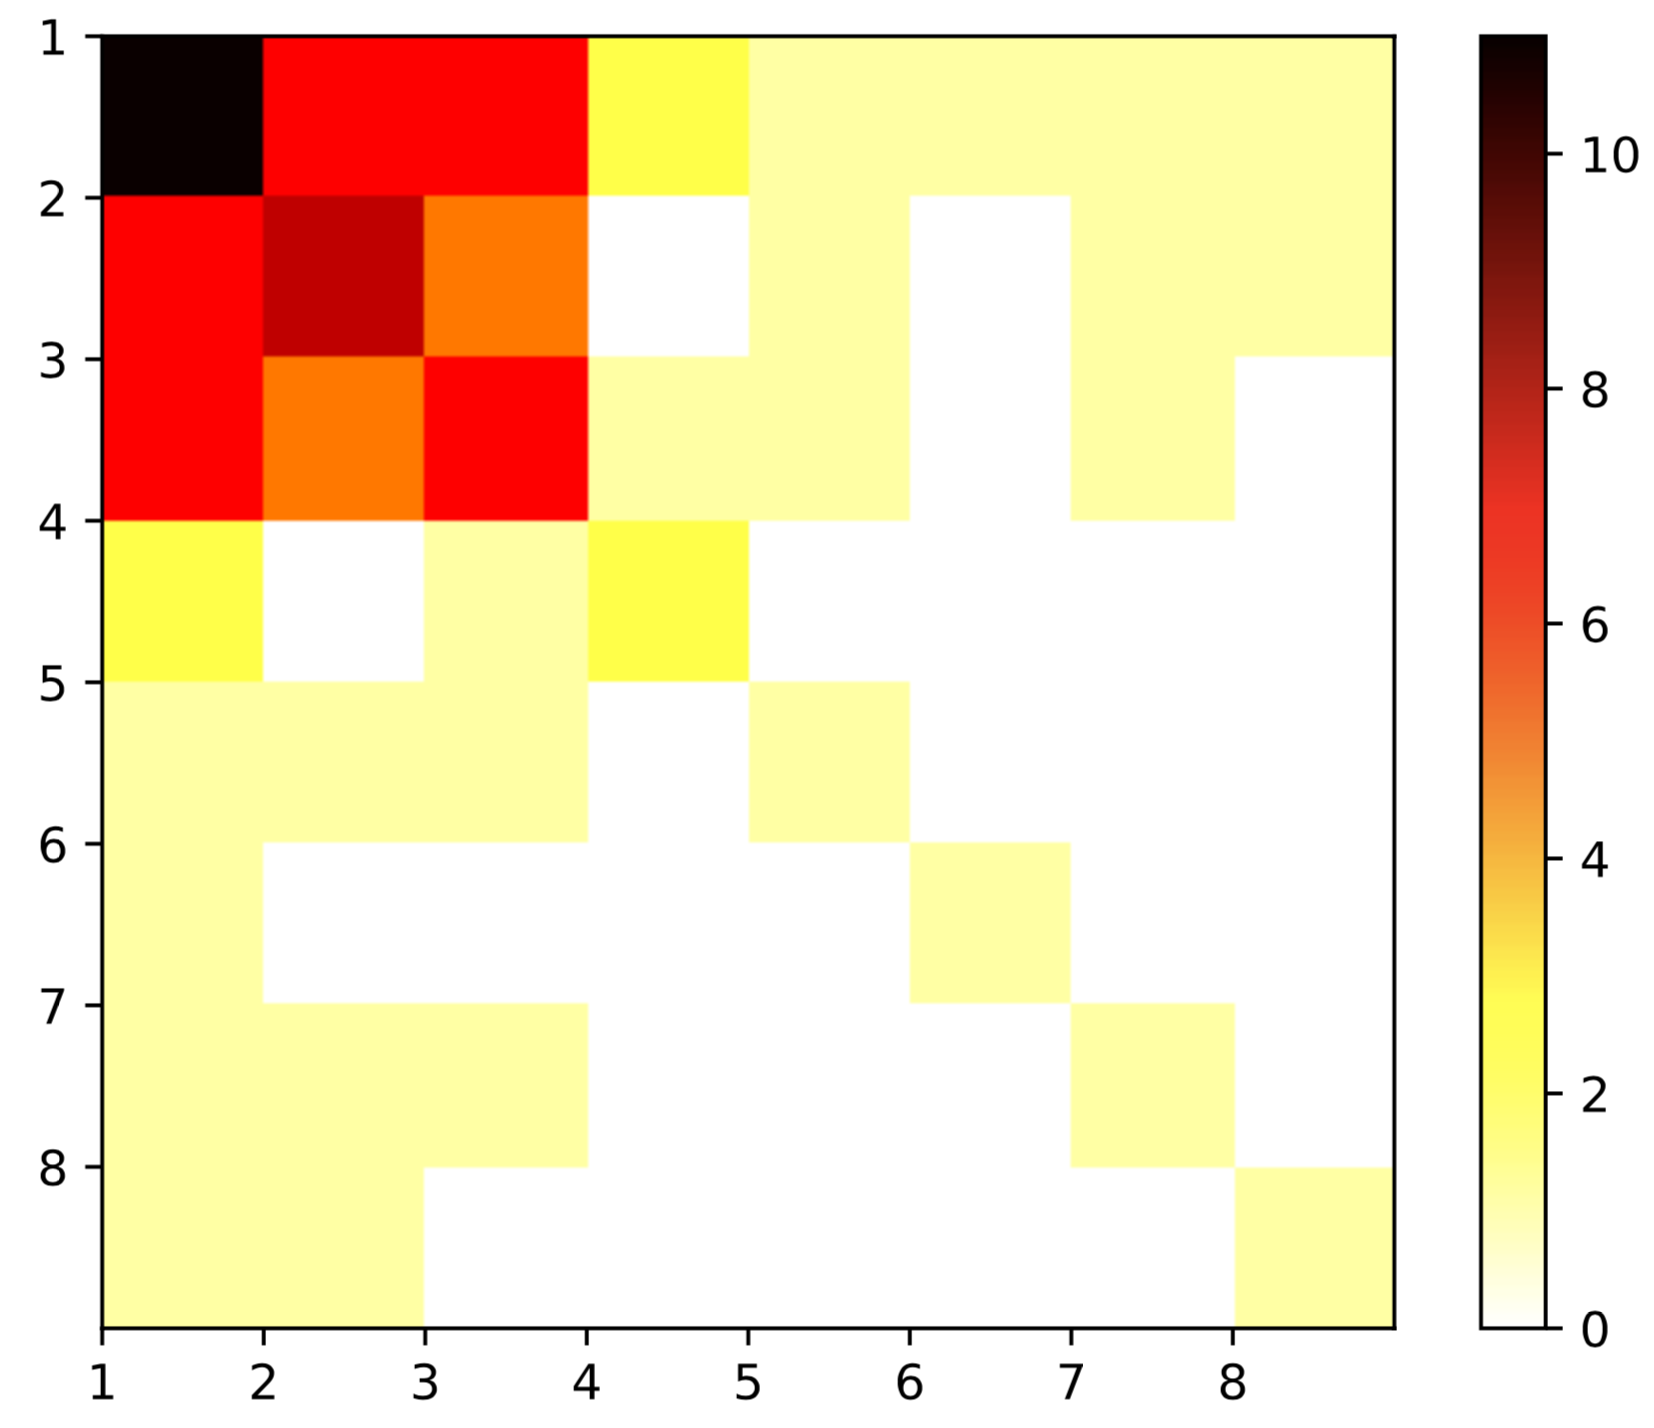
\includegraphics[width=1\textwidth]{img/motivation/tpc-h-orders}
        \caption{TDC-H中的 $orders$ 表。}
        \label{fig:h_count_cdf}
    \end{subfigure}%

    \begin{subfigure}[t]{0.5\textwidth}
        \centering
        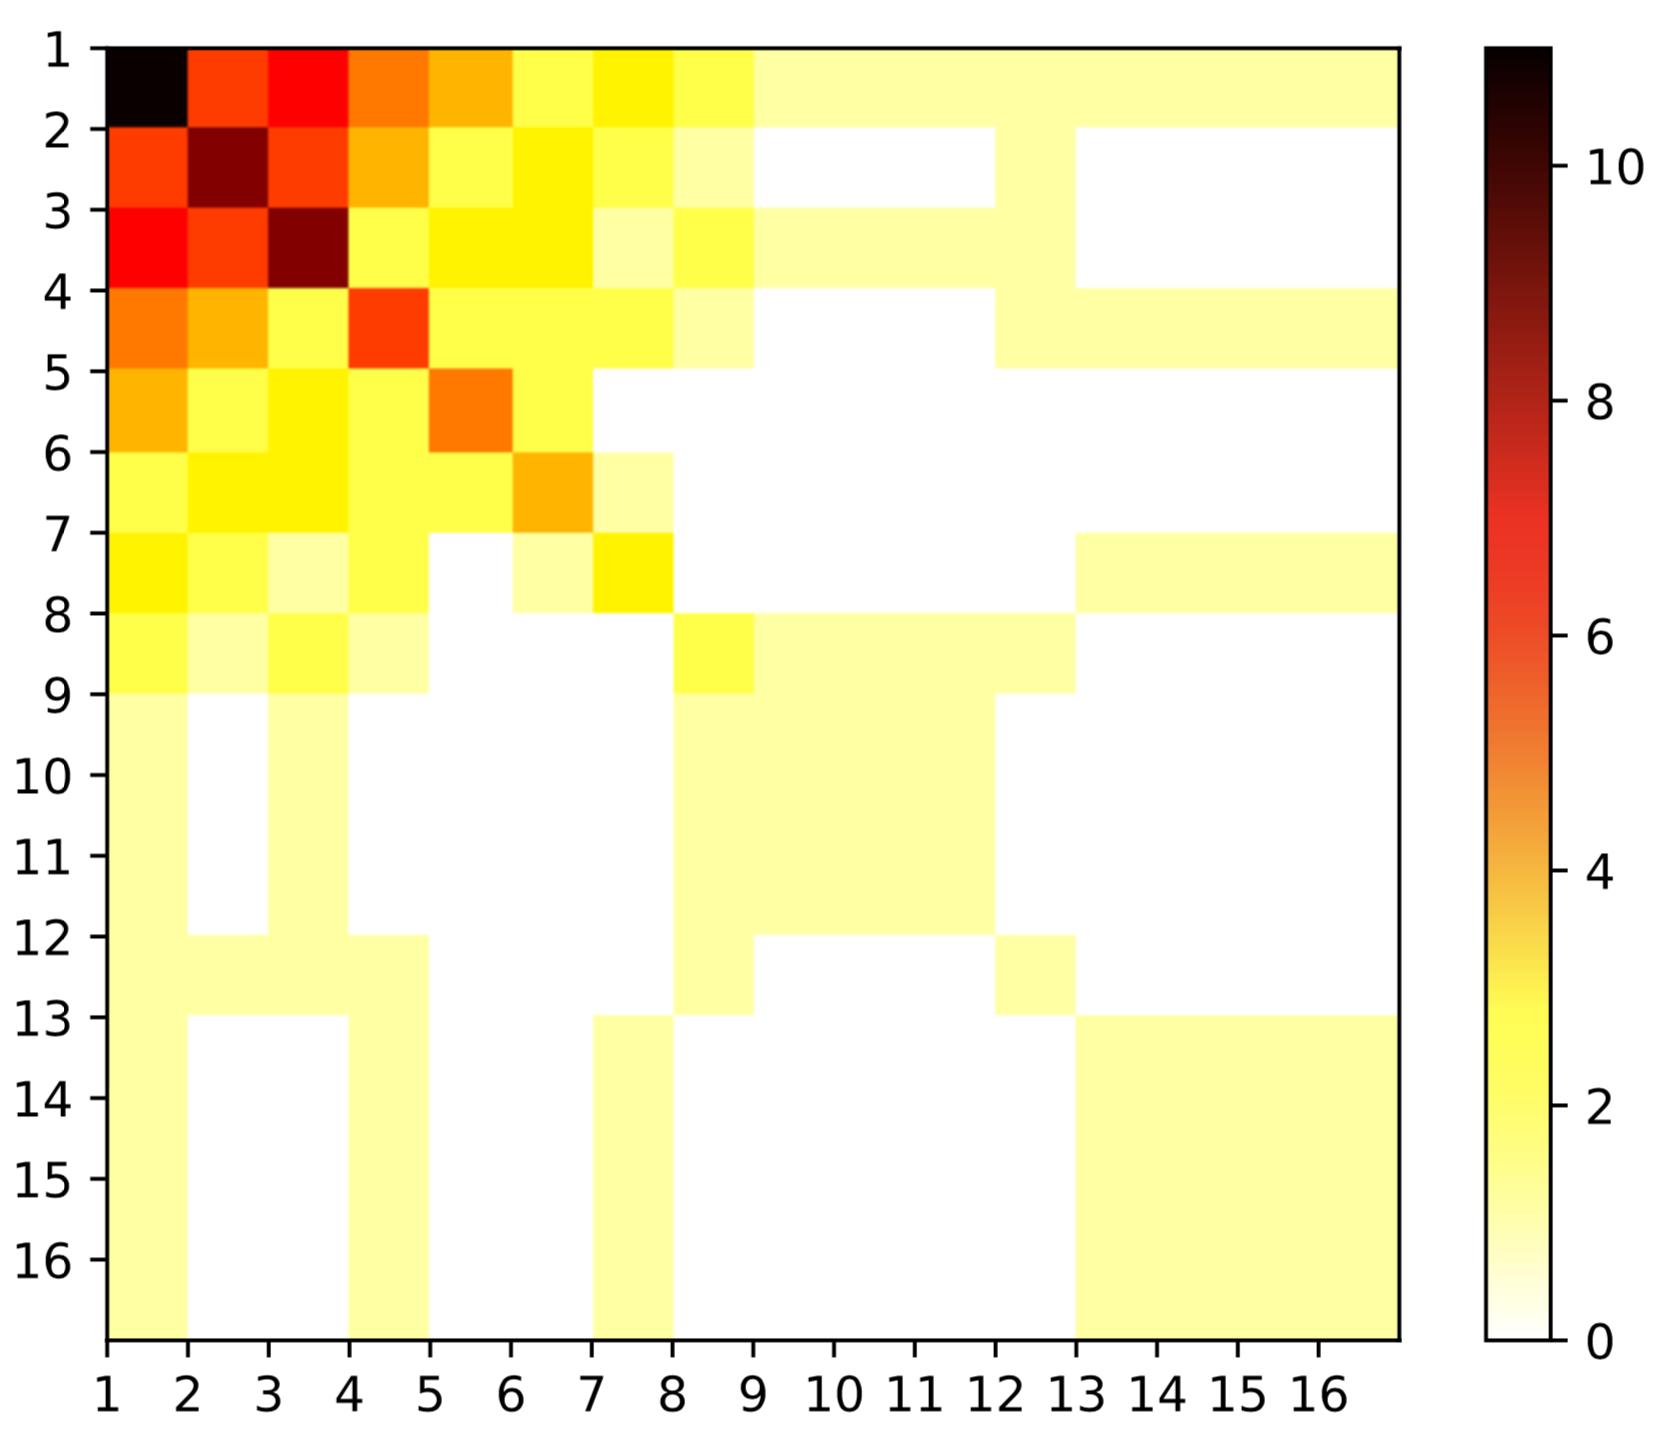
\includegraphics[width=1\textwidth]{img/motivation/tpc-bb-store_sales}
        \caption{TDC-xBB中的 $store\_sales$ 表。}
        \label{fig:bb_count_cdf}
    \end{subfigure}%
    \caption{三种标准测试程序中具有代表性的数据表的访问热图。}
    \label{fig:heatmap}
    %\vspace{-.1in}
\end{figure}

\section{列之间的数据shuffle}
\label{sec:data-shuffle}

\par 从~\ref{sec:col-access}节中观察到的现象我们获悉,每张数据表中一小部分的列非常热门,访问频率很高。如果我们复制这一小部分热门的列,并将它们缓存在不同的机器上,那么当SQL查询任务在分布式环境中执行时,这些热门的列很容易引起集群节点之间的数据shuffle。我们推测,这种shuffe给任务执行时间带来的影响是不可忽视的,为了展示列这一级别的网络开销,我们做了一个实验,测量一个小集群中列的热门程度与数据shuffle的关系。

\subsection{实验设置}
\label{subsec:data-shuffle-setup}

\par 我们部署了一个含有1个master和2个worker的小集群,所用的实例是c5.4xlarge,每一个有32 GB内存和16个CPU核,通过iperf3测试,小集群的网络带宽是10 Gbps。我们在集群上部署了Alluxio以及Spark,运行TPC-H标准测试程序。在实验中,只有一台worker缓存有6 GB的Parquet格式的数据,因此集群里每次执行查询任务都会引发从有数据的机器到没有数据的机器的数据shuffle。我们关闭了Spark和Alluxio的数据被动缓存功能,一个一个按顺序执行标准测试程序里的查询任务,保证每一次执行都会有数据shuffle。我们会记录每一列的总shuffle量。

\begin{figure}[htbp]
	\centering
	\begin{subfigure}[t]{0.5\textwidth}
		\centering
		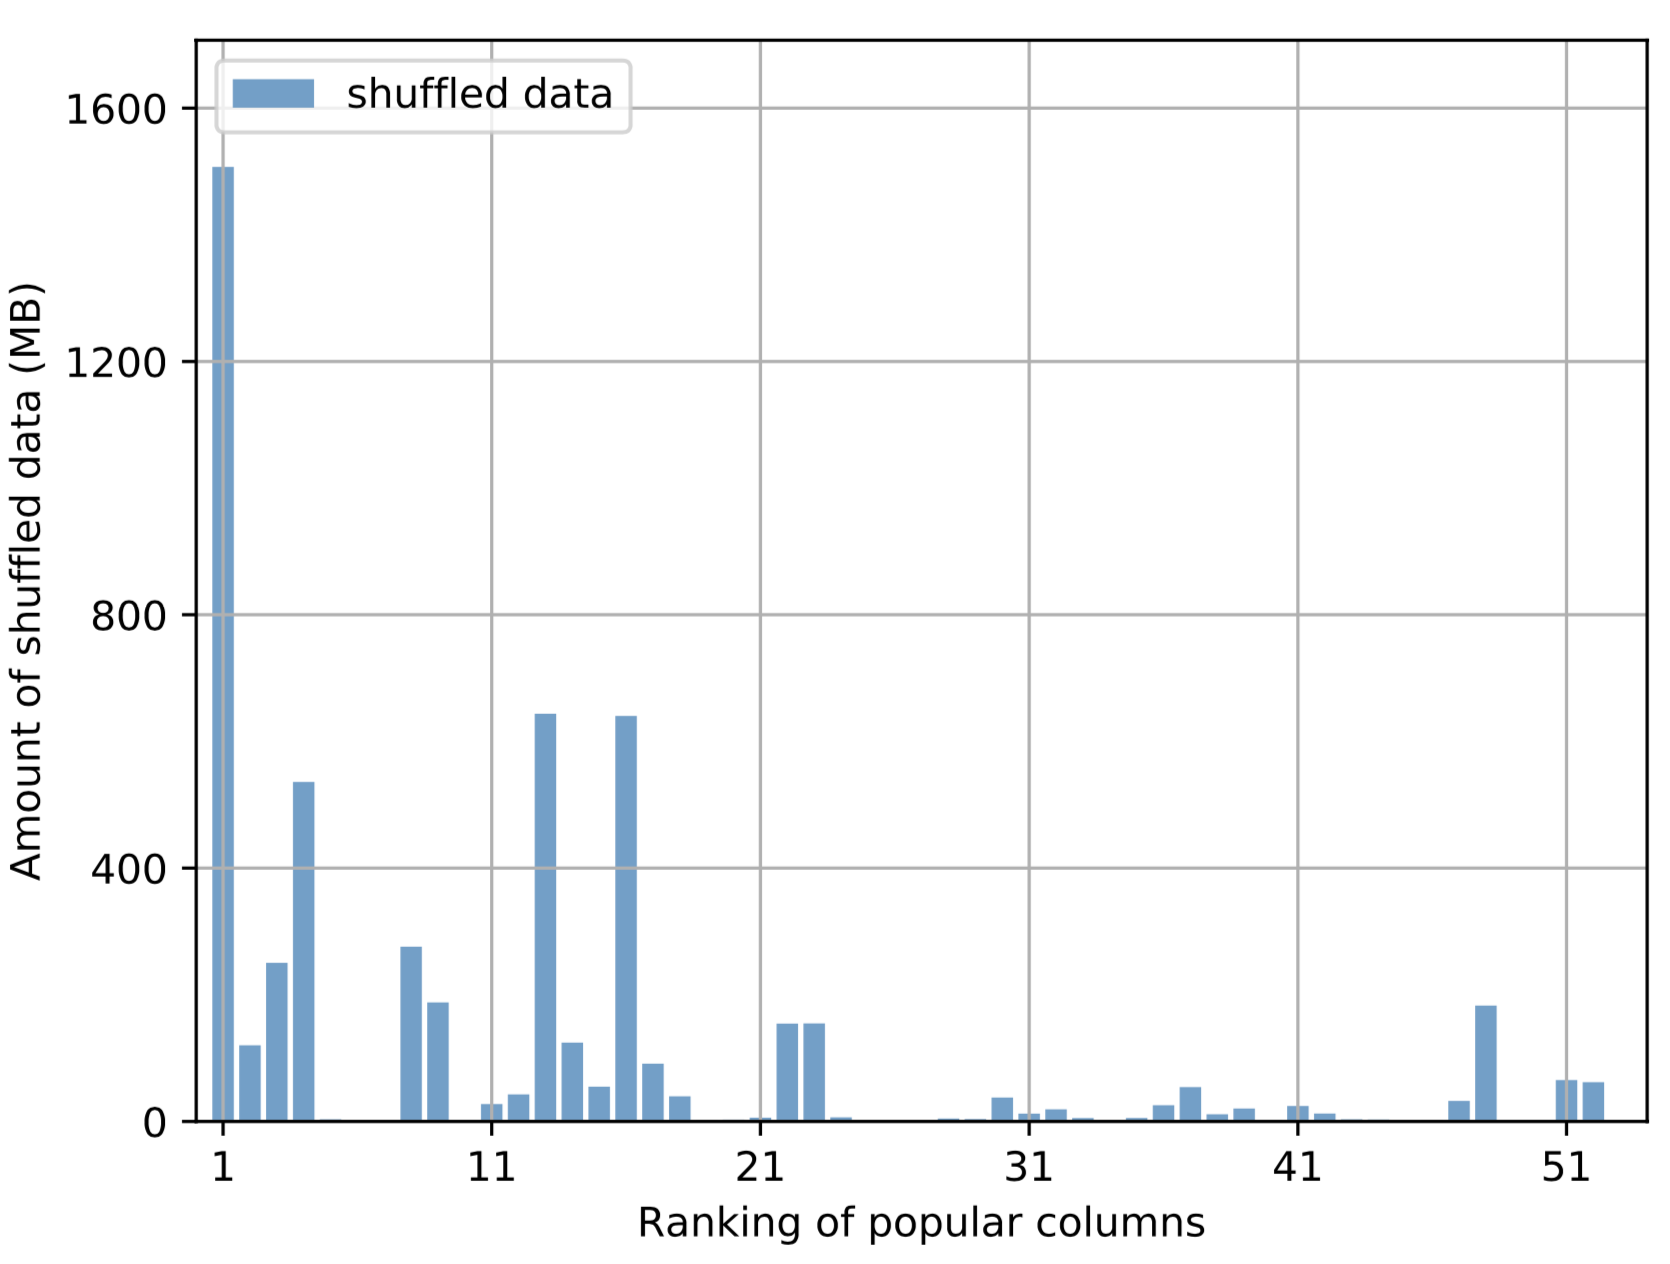
\includegraphics[width=1\textwidth]{img/motivation/pop-shf-a}
		\caption{每一列的总shuffle数据量。}
		\label{fig:pop-shf-a}
	\end{subfigure}%
	\begin{subfigure}[t]{0.5\textwidth}
		\centering
		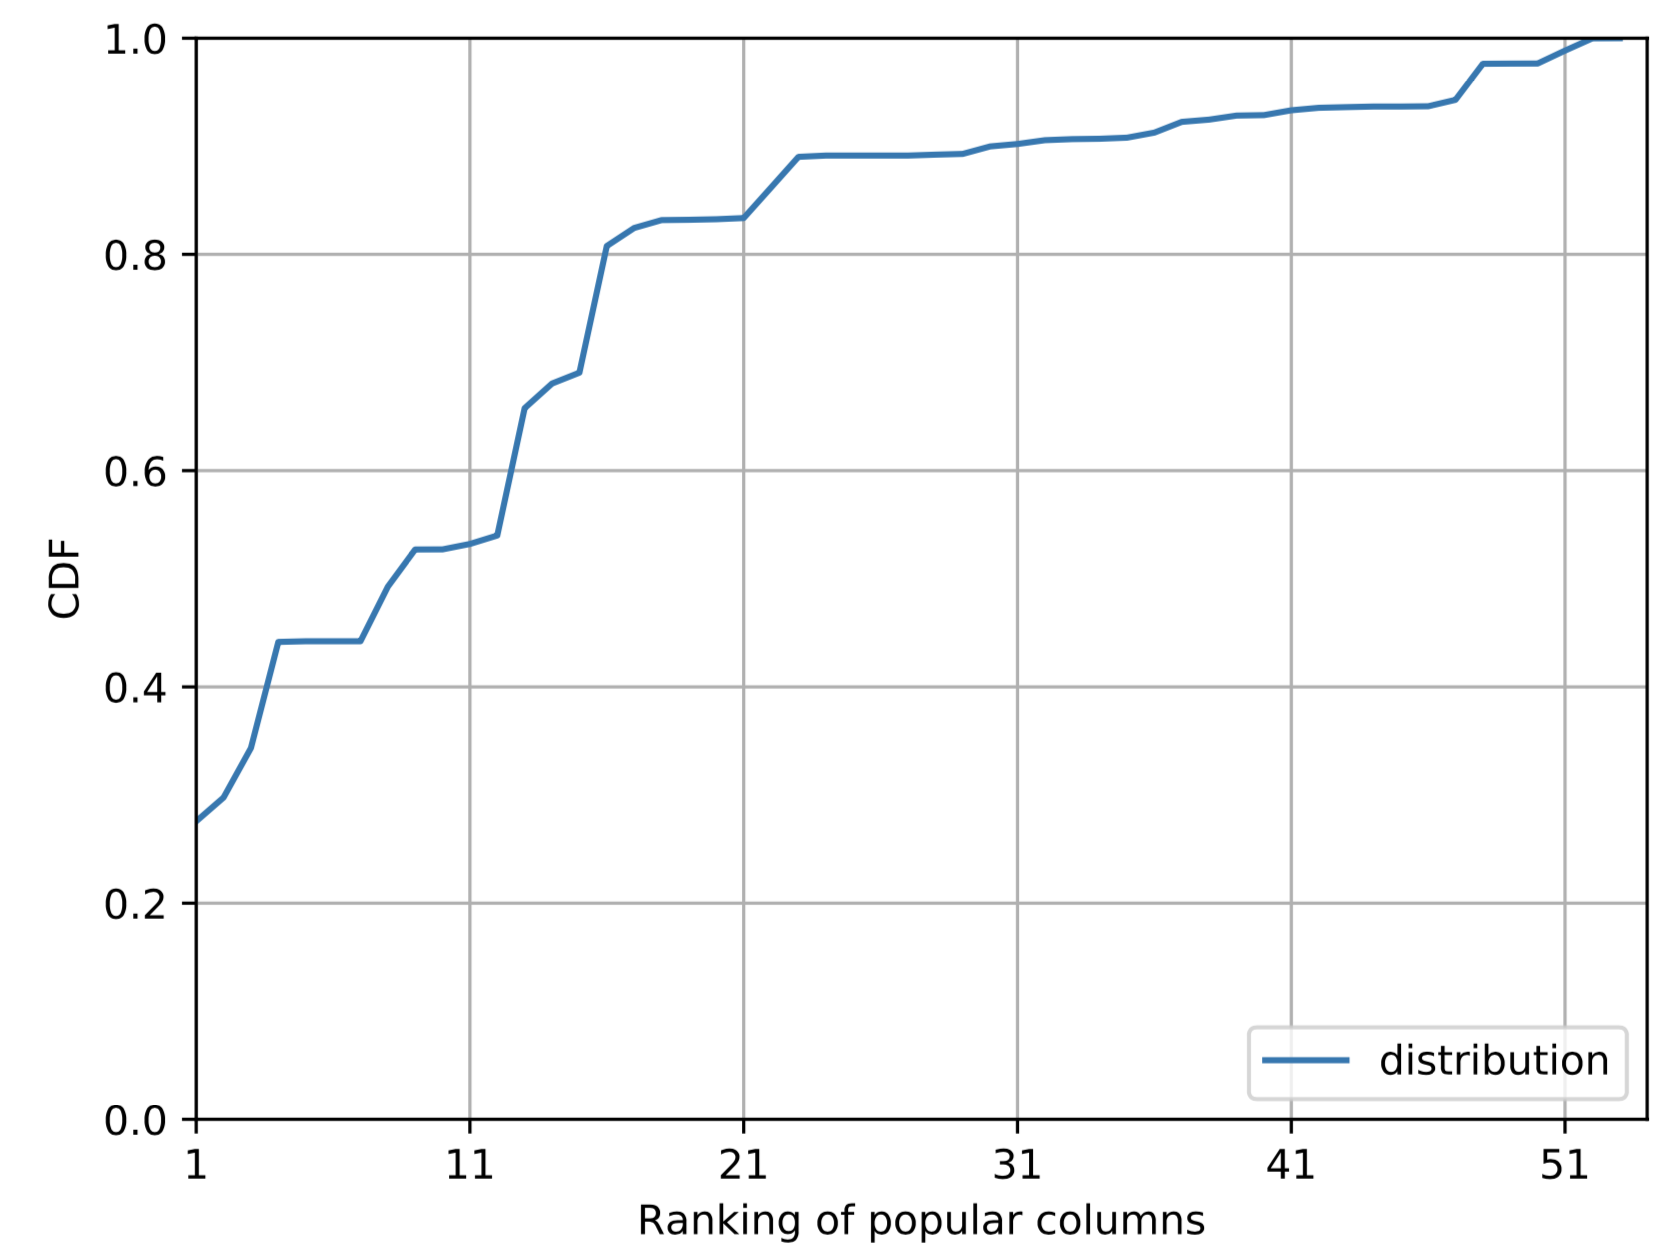
\includegraphics[width=1\textwidth]{img/motivation/pop-shf-b}
		\caption{列级别shuffle数据的CDF。}
		\label{fig:pop-shf-b}
	\end{subfigure}%
	
	\caption{TPC-H标准测试程序的列级别数据shuffle。}
	\label{fig:pop-shf}
	%\vspace{-.1in}
\end{figure}



\subsection{每一列的数据shuffle}

\par 图~\ref{fig:pop-shf}展示了上述实验的结果,其中图~\ref{fig:pop-shf-a}展示了列这一级别的数据shuffle量,TPC-H标准格式程序中的53列(所有表中的)按照它们的热门程度排序。因为热门的列被频繁访问,并且我们发现通常来说热门的列比冷门的列的体积更大,所以热门的列相比冷门的列引起更多的数据shuffle。根据图~\ref{fig:pop-shf-b}展示的分布,总体来说,查询任务产生的数据shuffle主要来自热门的列,比如接近90\%的数据shuffle量是由30\%最热门的列贡献的。

\section{数据shuffle的影响}
\label{sec:shuffle-impact}

\par ~\ref{sec:data-shuffle}节实验证明了热门的列很容易引起数据shuffle,本节中我们会用实验证明数据shuffle会降低执行查询任务的性能。

\subsection{实验设置}
\label{subsec:shuffle-impact-setup}

\par 这个实验所用的集群与~\ref{subsec:data-shuffle-setup}小节中描述的集群一致。我们设置了对照实验,其中实验组的设置与~\ref{subsec:data-shuffle-setup}小节一致,只把数据缓存在一台worker上,这一组会产生数据shuffle;另外一组中,我们将相同的数据在两台worker上均进行缓存,保证不会产生数据shuffle。我们对比两组中查询任务的执行时间,以此测量shuffle的开销。

\subsection{度量指标}
\label{subsec:shuffle-impact-metrics}

\par 我们使用任务的平均执行延迟\emph{slowdown}作为衡量指标:
\begin{equation}
    \text{Slowdown} = \frac{L_S - L_N}{L_N},
    %\text{Slowdown} = \frac{L_S - L_N}{L_N} \times 100\%,
\end{equation}

\par 其中$L_S$ 和 $L_N$ 分别是由shuffle和没有shuffle的实验中查询任务的执行时间。\emph{slowdown}的值越大表明其降低查询任务执行的性能的影响越显著。

\subsection{不同网络带宽下的shuffle开销}

\par 按照~\ref{subsec:shuffle-impact-setup}小节的设定,我们依次执行了TPC-H标准测试程序提供的查询任务并计算了每个查询任务的\emph{slowdown}(~\ref{subsec:shuffle-impact-metrics})。图~\ref{fig:cdf16-all}展示了网络带宽被限制为1 Gbps,3 Gbps和10 Gbps的情况下,\emph{salowdown}的分布。从图中可以看出,对于分布式环境下执行的SQL查询任务,网络是瓶颈,所以数据shuffle大大影响了任务执行的性能。例如,即便是在10 Gbps的带宽下,40\%的查询任务的延迟由于数据shuffle会上升10\%。此外,当网络带宽变得越小,shuffle带来的通信开销会更加明显,任务的性能的下降也会更加显著。



\begin{figure}[]
	\centering
	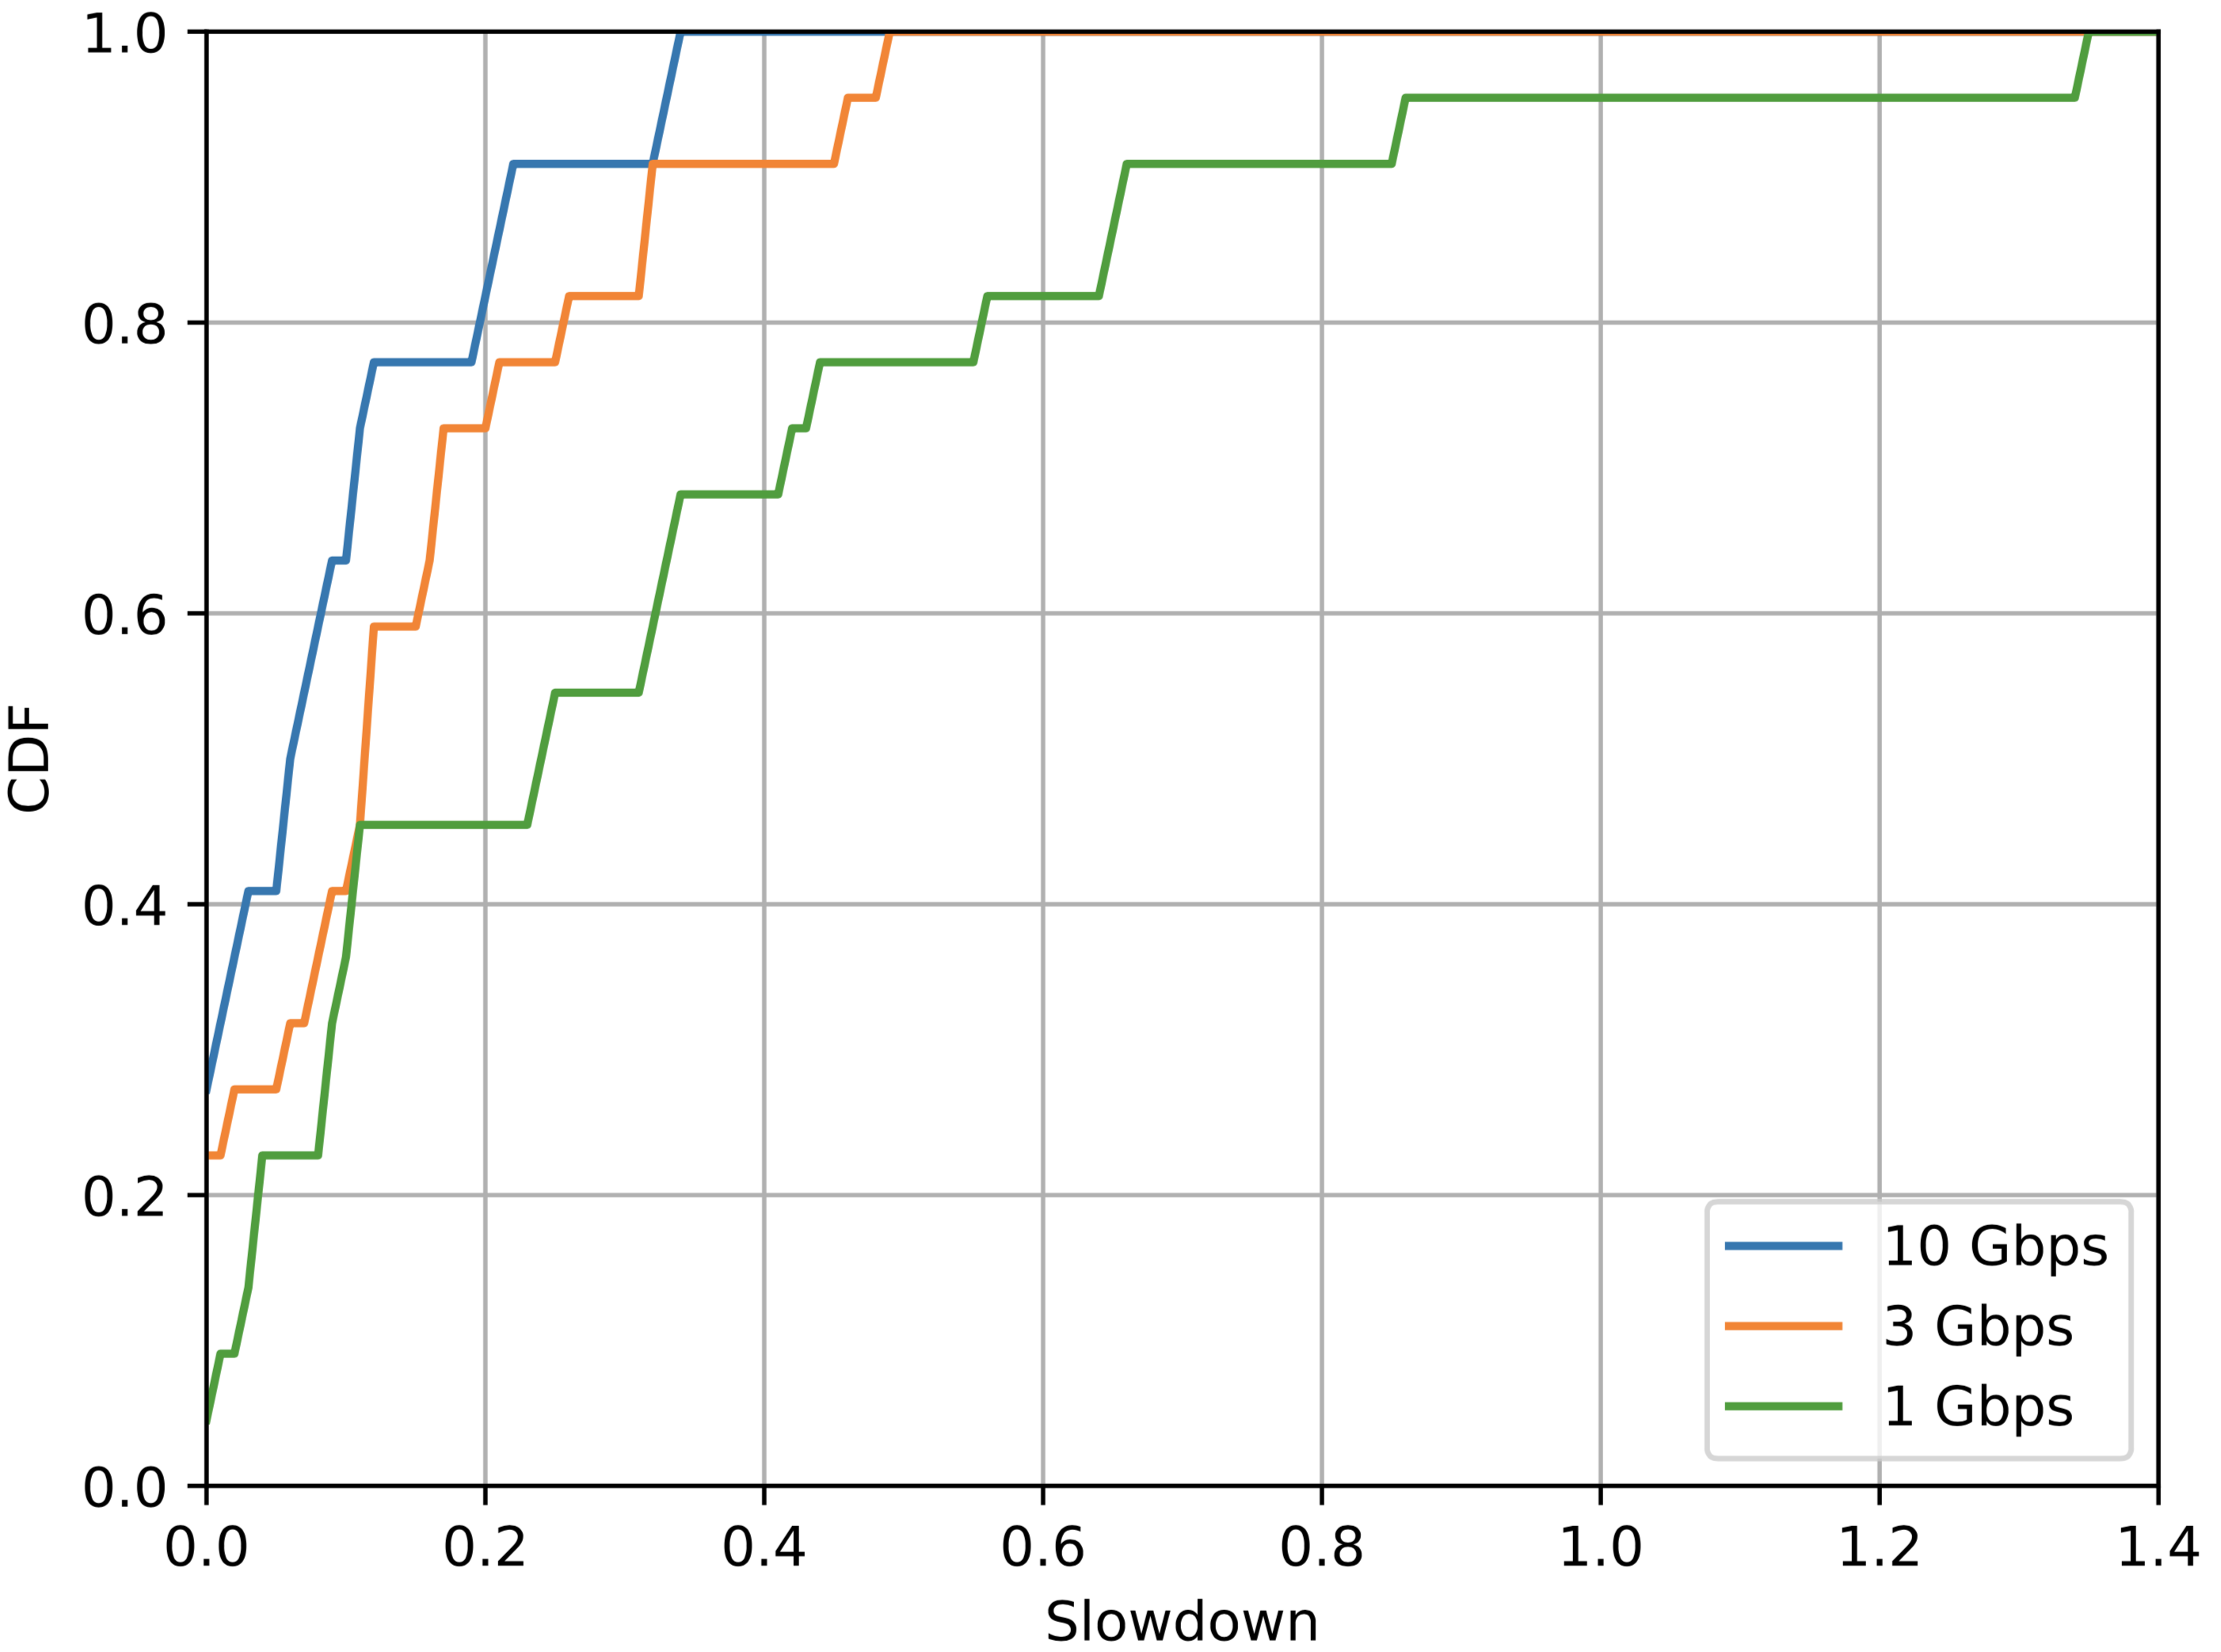
\includegraphics[width=0.5\textwidth]{img/motivation/cdf16-all}
	
	\caption{slowdown在不同网络带宽下的分布。}
	\label{fig:cdf16-all}
	%\vspace{-.1in}
\end{figure}

\section{总结}

\par 我们从本章第~\ref{sec:col-access}节得知,一张数据表中不同列之间热门程度(访问频率)存在明显的差异,且当考虑两两之间被共同访问的概率时,两列的热门程度越高,二者被共同访问的频率越高。在一张表中,热门的列是少数,其余多数是冷门的,不经常被访问。我们这些规律可以推断,相比对整张数据表进行复制,理论上复制数据表里相对热门的若干列能够达到接近复制整表的负载均衡的效果。因为冷门的列本身访问次数不多,在较长的一段周期内,热门的列的访问负载由其副本承担,而冷门的没有被复制的列的访问负载由原表承担,直观来说,这能够起到不错的负载均衡效果。与此同时,复制更少的列,降低缓存开销。提高缓存效率。

\par 将热门的列分别复制,如果随机放置在缓存服务器上,那么一个查询任务很容易引起表内部的数据shuffle,因为各个列的副本很有可能不在同一台服务器上。第~\ref{sec:data-shuffle}节显示,通常来说,热门的列引起的数据shuffle的量更大,第~\ref{sec:shuffle-impact}节证明,表内部的数据shuffle对于查询任务的执行时间的影响是不可小觑的。

\par 以上总结告诉我们,设计方案时我们需要考虑:第一,哪些列是热门的列,需要复制多少热门的列;第二,复制以后,这些列在集群里如何放置,这涉及到“捆绑”(bundle)放置的问题。
\chapter{Column-aware方案与缺点}
\label{chp:column-aware}

\par 在本章中我们会讨论一个容易想到的直接的方案,取名Column-aware方案,此方案没有考虑工程实现的难度,仅考虑我们的目标。然后本章会讨论我们的现有条件,分析这个方案存在的缺点,不能在实际中应用的原因,为我们的第~\ref{chp:cw-cache}章提出的应用Bundle-K方案的CW-Cache系统提供参考。

\section{Column-aware方案}

\par 由第~\ref{chp:motivation}章我们知道,设计方案时需要考虑如何决定复制多少热门的列,以及列的“捆绑”(bundle)放置问题。那么,根据先前的分析,从直观上来说,想要基于列的访问热度对集群缓存系统实现列级别的负载均衡,我们的系统需要获得SQL查询任务具体访问的列,才方便对列的热度进行统计,并且根据此热度信息对热门的列进行复制。应用访问数据表的列的信息是由上层计算框架(如Spark SQL)掌握,而alluxio是不知道的,需要计算框架提供给它,拿到这些信息之后,alluxio进行统计,计算列的访问热度,根据热度,计算列需要拷贝的副本数,访问到来时,alluxio根据一定的策略,返回副本中的一个(如果被复制)或者是原表。

\par 图~\ref{fig:sim-archi}所示即为本章描述的Column-aware方案的架构的设计。该架构主要有三大组件,最上层计算框架为Spark SQL~\cite{spark-sql}(也可以更换为其他的),中间是基于alluxio\cite{alluxio}实现的列级别的负载均衡系统CW-Cache,底层是分布式文件系统HDFS(Hadoop File System)\cite{hdfs}。

\begin{figure}[]
	\centering
	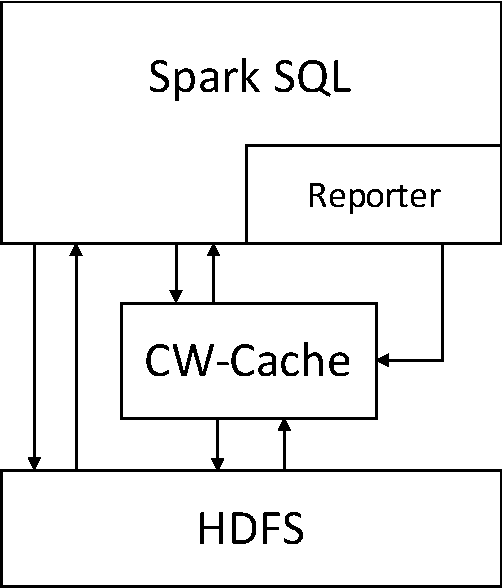
\includegraphics[width=0.4\textwidth]{img/column-aware/sim-archi}
	
	\caption{Column-aware方案的架构设计。}
	\label{fig:sim-archi}
	%\vspace{-.1in}
\end{figure}

\par 这个采用Column-aware方案的负载均衡系统CW-Cache工作流程大致如下:当用户给Spark SQL提交一个查询任务,经过一系列转换后,Spark SQL得到具体要访问的列的信息,Reporter负责将这些信息传递给CW-Cache,CW-Cache记录下这些信息,并且将对应列的访问计数器加1。在经过一段时间后,CW-Cache对于缓存的数据表的各个列,均维持有计数器,从中获得各个列的热度(访问频率),然后它根据一定的算法计算出哪些列需要进行复制,复制多少份,哪些列需要“捆绑”在一起放置。当查询任务再次到来,CW-Cache得到应用访问的列,CW-Cache根据一定的策略,在缓存副本(如果有)或者原表中选择相应的列的信息返回给应用,尽可能使得负载比较分散,并且尽力避免出现shuffle,同时更新相关列的访问计数器。以上步骤重复进行。

\par 这个系统是根据我们的目标的很直接简单的一种思路,但是它是不实用的,首先这样的设计不够通用,比如图~\ref{fig:sim-archi}是针对Spark SQL进行了修改的,如果更换SQL引擎又需要重新实现;其次,这样的设计需要对上层计算层和中间层同时做修改,增加了二者的耦合度,不利于软件开发与维护。下面我们会分析现有条件Parquet和alluxio来解释以上原因。

\section{现有条件}

\subsection{Parquet文件格式}

\par 列式存储有多种格式,其中一种被广泛使用的具有代表性的列式存储的文件格式是Parquet,我们的方案针对Parquet实现,所以在这里我们具体讨论一下Parquet格式。

\par Parquet文件是以二进制方式存储的,因此不能够像文本文件一样直接读取,Parquet中包括该文件的元数据(metadata)和数据,所以Parquet格式的文件是自解析的。在Hadoop File System文件系统和Parquet文件中有以下几个概念。

\begin{itemize}
    \item HDFS文件(File):一个HDFS文件包括数据和元数据,数据分散地存储在若干个HDFS块(Block)中。

    \item HDFS块(Block):HDFS块(Block)是HDFS上最小的副本(replica)单位,HDFS会把一个Block作为一个文件存储在本地,并且维护分散在不同的机器上的多个副本(默认每个文件3个副本)。Block的大小可以根据需求由用户自己配置,Hadoop早期版本默认一个Block大小是128M,Hadoop 2.7.3以及之后的版本默认一个Block的大小为128M。
    
    \item 行组(Row Group):Parquet按照行(Row)将数据从物理上划分为多个单元,每一个行组包含一定的行数,每一个HDFS文件至少存储一个行组,Parquet读写的时候会将整个行组缓存在内存中,所以每一个行组的大小是由内存容量决定的,也就是说记录(Record)占用空间比较小的Schema可以在每一个行组中存储更多的行。

    \item 列块(Column Chunk):在一个行组中,同一列储存在一个列块中,行组中的所有列依次连续地存储在这个行组中。同一个列块中的值的类型是相同的,不同的列块可能使用不同的压缩算法进行压缩。

    \item 页(Page):每一个列块划分为多个页,页是最小的编码的单位,同一个列块中的不同页可能使用不同的编码方式。
\end{itemize}

\par 一般情况下,在存储Parquet数据的时候会根据下层文件系统的块(Block)大小来设置行组的大小,在MapReduce计算框架中,由于一般情况下每一个Mapper任务处理数据的最小单位是一个块(Block),这样可以把每一个行组由一个Mapper任务处理,提高任务执行并行度。Parquet文件的格式如下图~\ref{fig:parquet-file-layout}所示。


\begin{figure}[]
	\centering
	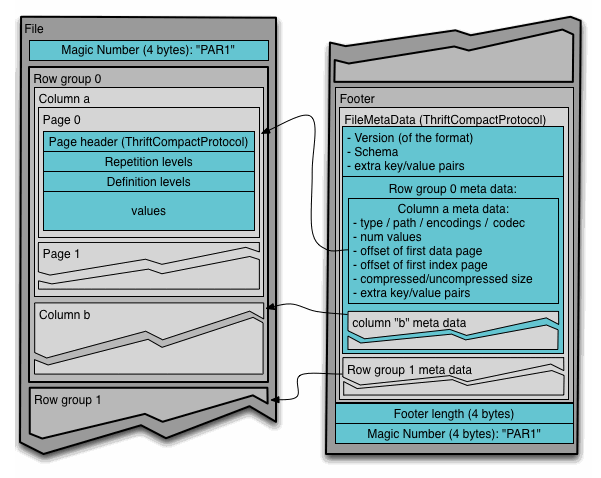
\includegraphics[width=0.5\textwidth]{img/column-aware/FileLayout}
	
	\caption{Parquet文件格式。}
	\label{fig:parquet-file-layout}
	%\vspace{-.1in}
\end{figure}

\subsection{Alluxio}
\label{subsec:alluxio}

\par Alluxio原名Tachyon,是一个基于内存的分布式文件系统,它是架构在底层的分布式文件系统(如Amazon S3、Apache HDFS等)和上层分布式计算框架(如Spark、MapReduce、Hbase、Flink等)之间的中间层,主要职责是以文件形式在内存或其它存储设施中提供数据的存取服务。在Alluxio出现以前,这些上层的分布式框架,往往都是直接从底层的分布式文件系统中读写数据,效率比较低,性能消耗比较大,而如果将Alluxio部署在二者之间,以文件的形式在内存中对外提供读写访问服务,那么Alluxio可以为这些大数据应用提供一个数量级的加速,而且它提供通用的数据访问接口,所以能够很方便地切换底层的分布式文件系统。

\begin{figure}[]
	\centering
	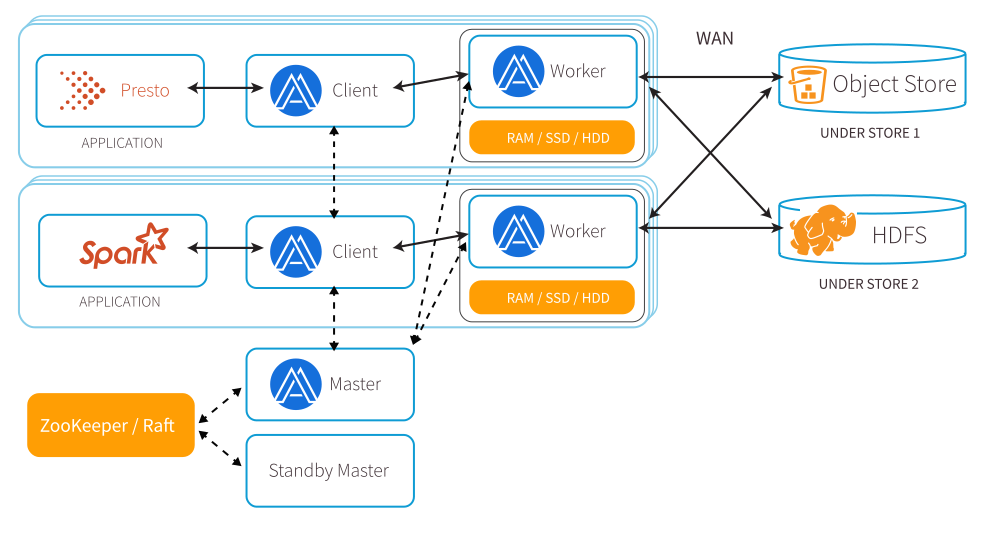
\includegraphics[width=0.8\textwidth]{img/column-aware/alluxio-archi}
	
	\caption{Alluxio架构。}
	\label{fig:alluxio-archi}
	%\vspace{-.1in}
\end{figure}

\par Alluxio的架构如图~\ref{fig:alluxio-archi}所示。整体框架为主从结构,与Hadoop\cite{hdfs}等类似。主节点为Master,负责管理全局的文件系统的元数据,比如文件系统树等;从节点运行Worker进程,负责管理本节点的数据存储服务;Client用于Alluxio与用户应用的交互,为用户提供统一的文件存取服务接口。

\par 当应用程序需要访问Alluxio中存储的文件,先通过Client客户端与主节点Master通讯,待Master返回存储有应用需要的文件的worker列表,再根据一定的策略和对应Worker节点通讯,进行文件的存取操作。所有的Worker会周期性地发送心跳消息给Master,维护文件系统的元数据信息,确保自己被Master感知而仍然能在集群中正常提供服务。Master不会主动发起与其他组件的通信,它只是以回复请求的方式与其他组件进行通信。这与HDFS、HBase等分布式系统设计模式是一致的。

\subsection{分析}
\label{subsec:simp-analysis}

\par 从上文的分析可以看出,Parquet文件格式在存储数据表时,先将数据表按行“切割”出一个个行组(Row Group),行组内部再按列分成列块(Column Chunk),文件系统里物理存在的文件含有若干行组,同一列的数据在物理上并没有存储在一起,并且不同的块(Block)有可能放置在不同的机器上。按照我们在本章提出的Column-aware方案,CW-Cache能够获得Parquet文件的语义信息,希望把热门的列单独提取出来,但是考虑到Parquet文件的文件格式,我们认为这个目标的实现不太容易。直观上来说,需要读取Parquet文件的元数据,找出需要复制的列所在的Block,读取之后将它们拼装成一个新的文件,进行复制,这个过程的产生不可忽略的计算开销和网络通信开销,可能对系统性能造成比较大的影响,抵消因负载均衡获得的性能提升。

\par Spark SQL能解析基本的SQL语句并在分布式环境下高效执行,当Spark SQL解析出查询任务需要访问的列,具体的读取任务是交由Parquet文件格式的实现parquet-mr\cite{parquet-mr}来完成的,parquet-mr会读取Parquet文件的footer获取文件的元数据,定位需要读取的列所在的文件块(block)、偏移(Offset)和读取的长度(Length)。然后它把这些信息传递给alluxio,alluxio将结果返回给parquet-mr,parquet-mr将数据解压缩(如果进行了压缩)、拼装之后交给应用进行处理。单独看这个过程,alluxio拿到的信息是一个个“文件片段”,它们甚至不是完整的列块(column chunk),可能只是其中的一小部分,有时为了高效读取数据,parquet-mr甚至并行地一个一个字节读取文件。本章Column-aware方案需要alluxio获得应用读取Parquet文件时的关于列的语义信息,而alluxio本身的架构决定了它并不支持这一点,很难将这些零碎的“文件片段”与Parquet存储的数据表的各个列建立关联。如果想要向alluxio传递文件的上下文信息,我们需要额外修改Spark SQL或者parquet-mr的相关模块,增加了上层计算框架和中间层的耦合度,同时因为只在Spark SQL或者parquet-mr进行修改,那么方案仅仅适配Spark SQL计算框架或者Parquet这种文件格式,没有通用性,是不好的软件设计。

\par 此外,列的“捆绑”放置(bundle)也是非常困难的。根据~\ref{sec:data-shuffle}和~\ref{sec:shuffle-impact}节,将数据表以列为单位分开缓存且分开放置会在查询任务中引起数据表内部的shuffle,且shuffle带来的网络通信开销会对查询任务的执行时间带来不可忽视的影响。~\ref{sec:col-access}节的实验结果表明在列的热度存在倾斜的基础上,不同热度的列相互之间被共同访问的概率也不一样。于是我们想到可以借助“捆绑”放置(bundle)来减少甚至避免同一张数据表内的数据shuffle。然而这个问题是难以解决的:首先如何得到列的共同访问的模式是困难的。如果一张数据表有$N$列,那么列的共同访问的模式理论上有$2^N$种,在生产环境中是没有足够的资源来同时满足这么多共同访问模式。其次,从系统上来说,alluxio作为通用的内存分布式文件系统,需要为多用户提供服务,只要用户通过alluxio的接口存取文件,alluxio便执行相应的操作,将结果返回即可。alluxio并不知晓每一次的请求来自哪个客户端(Client),Master端不会维护状态,区分不同客户端的请求。换句话说,不做修改的情况下,alluxio无法得知哪些读访问请求来自同一个客户端的同一个查询任务,那么列的“捆绑”(bundle)放置也就无从谈起。而如果要使得alluxio维护状态信息,首先需要客户端发送请求时附带自己的身份信息,同时alluxio的master需要记录并且进行匹配,大大增加系统的网络、存储、计算开销。

\section{总结}

\par 本章主要讨论了一个不考虑系统实现,只针对列级别负载均衡目标的集群缓存系统Column-aware方案,它需要上层计算框架将访问的列的信息发送给中间层CW-Cache,CW-Cache借此统计各个列的访问热度,并且按照一定的策略复制,在请求到来时选择合适的副本传给应用。这个方案有三点缺陷。

\begin{enumerate}
    \item 因为Parquet文件格式是先按照行进行划分,然后再按列进行存储,如果要按照需求把某一列单独提取出来进行复制,需要读取文件元数据、读取存储该列的各个Block,然后拼装成新的Parquet文件存放到其他机器,这一系列的操作开销较大;
    \item Spark SQL读取Parquet文件时,调用parquet-mr,传给alluxio的信息仅有所需的文件URI(统一资源标识符)、偏移量和读取长度,并未包含文件的语义信息。想要传递文件上下文信息需要额外对Spark SQL或者Parquet-mr做修改,增加了软件之间的耦合度;
    \item Alluxio作为通用的内存文件系统,为多用户提供服务,不保存状态信息,不去识别请求来自哪个Client,这意味着alluxio难以知晓对哪些列的访问是来自于同一个Client的同一个查询任务,不便于对这些列的缓存作“捆绑”放置(bundle)。如果访问文件时增加Client的身份标识,会大大增加通信开销,同时增加Master维持状态信息的存储、计算开销。
\end{enumerate}

\par 综上所述,本章描述的采用Column-aware方案的系统开发难度较大,结构设计不合理,实用性相对较差,但对其缺陷的分析有助于我们更加深刻的理解问题,在现有条件的基础上调整系统设计的方向。在第~\ref{chp:cw-cache}章中我们会介绍本项目中CW-Cache系统实际采用的Bundle-K方案的设计与分析。
\chapter{CW-Cache:设计与分析}
\label{chp:cw-cache}

\par 根据第~\ref{chp:simple-solution}章对简单方案的分析,我们了解到我们的方案需要根据数据表中各个列的热门度(访问频率)决定哪一些列需要被复制,复制多少份,此外根据第~\ref{chp:motivation}章的分析,复制后的列的副本分开存储,执行SQL查询任务时会引起shuffleing,且shuffling会对任务执行时间产生不可小觑的影响,我们设计的方案需要尽力避免。本人的毕业设计是实验室项目组的一部分,此项目还在进行中,在这个毕业设计中我会展示目前其中的一种设计方案,接下来我会对此方案进行数学建模与分析。

\par 我们称这个方案为“Bundle-K”,正如字面意思所示,我们经过统计后将数据表中的各个列按照热度(访问频率)进行排序,然后“捆绑”前$K$个列进行复制。在执行查询任务的时候,如果查询任务涉及的所有列均在这复制出来的前$K$个列中,那么就由副本为查询任务提供数据,否则就由原表为任务提供数据。

\section{问题建模}
\label{sec:bundle-k-model}

\par \noindent \textbf{符号定义} \quad 这里我们对一张数据表内的列级别的共同访问模式进行描述。假设这张表共有$n$列,记为 $\left\{c_{0}, c_{1}, \dots, c_{n-1}\right\}$ ,它们所占空间的归一化分别是 $\left\{s_{0}, s_{1}, \dots, s_{n-1}\right\}$ ,则 $\sum_{i=0}^{n-1} s_i = 1$ ,一些查询任务会访问一组特定的列,我们称这一组列是一个共同访问模式。假设有$m$个共同访问模式 $T = \left\{t_{0}, t_{1}, \dots, t_{m-1}\right\}$ ,对于某一个特定的访问模式$t_i$,它的热度$p_i$代表了有这个访问模式的查询任务的数量,$ts_i$是这个访问模式中所有列的大小之和。这$m$组共同访问模式的负载分别是 $\left\{l_{0}, l_{1}, \dots, l_{m-1}\right\}$ ,其中 $l_i = p_i ts_i$ 。

\par 记$k$为复制的最热门的列的数量,$S_k$是这复制的$k$列组成的副本能够覆盖的访问模式的集合,那么所有的访问模式就被分成了两组,$S_k$和$T-S_k$。记$L_h$和$L_c$分别是$S_k$和$T-S_k$承担的总负载,则有 $L_h=\sum_{i \in S_{k}} l_{i}$ 以及 $ L_c = \sum_{i \notin S_{k}} l_{i}$。

\par 假设我们的集群有$N$台服务器,我们的目标是找到$k$和副本的数量$r$来最小化任意一台服务器的\emph{负载的方差}和\emph{复制的代价}。


\par \noindent \textbf{目标} \quad  记$X$是任意一台服务器的负载,那么

\begin{equation}
    X=a_{0} \frac{L_{h}}{r}+a_{1} L_c,
\end{equation}

\par 其中$a_0$ 和 $ a_1$ 是二元随机变量,表示一个副本/原表是否被放置在这台机器上。由于我们将副本和原表随机放置在集群中,$a_0$ 和 $ a_1$ 服从伯努利分布且相互独立,因此我们能够得出:

\begin{equation}
\begin{split}
\operatorname{Var}(X)&=\frac{L_{h}^{2}}{r^{2}}\frac{r}{N}\left(1-\frac{r}{N}\right)+L_{c}^{2}\frac{1}{N}\left(1-\frac{1}{N}\right) \\
& = \frac{1}{N}\left(\frac{L_{h}^{2}}{r}+L_{c}^{2}\right) - \frac{1}{N^2}\left( L_h^2 + L_c^2\right)
\end{split}
\end{equation}

\par 记 $C$ 为复制的代价,即缓存这些副本占用的内存空间,我们有:

\begin{equation}
    C = r \sum_{i=0}^{k-1} s_i
\end{equation}

\par 我们的目标是使得负载的方差与复制的代价的加权和最小化。假设权重为 $w$,那么:

\begin{equation}
\label{eq:obj}
\begin{aligned}
\min \quad & \frac{1}{N}\left(\frac{L_{h}^{2}}{r}+L_{c}^{2}\right) - \frac{1}{N^2}\left( L_h^2 + L_c^2\right) + w\times r \sum_{i=0}^{k-1} s_i\\
\textrm{s.t.} \quad & k \in \{1, \cdots, n\}\\
& r \in \{1, \cdots, N\}    \\
\end{aligned}
\end{equation}

\section{算法}

\par 我们可以通过遍历所有可能的值,即从1到n,来寻找最佳的$k$。具体来说,对于每一个可能的$k$值,我们那更新$S_k$来计算$L_h$ 和 $L_c$,接着我们计算当前的$k$值下最优的$r$值。用$f(r)$并表示目标函数,我们能够发现:

\begin{equation}
f'(r) = - \frac{L_h^2}{Nr^2} + w\sum_{i=0}^{k-1} s_i
\end{equation}
\par 当 $f'(r) = 0$,可以得到:
\begin{equation}
\label{eq:r}
r = \sqrt{\frac{L_h^2}{N w \sum_{i=0}^{k-1} s_i}},
\end{equation}

\par 在这个例子中,我们的目标函数$f(r)$能够求到最小值。

\begin{algorithm}[tb]
	\caption{Find optimal $k$ and $r$}
	\label{alg:algo}
	\small
	\begin{algorithmic}[1]
		\Statex{-- $T$: 所有的共同访问模式}
		\Statex{-- $l[0\cdots m-1]$: $m$ 个访问模式的负载}
		\Statex{-- $w$: 最小化目标函数(等式~\ref{eq:obj})中的权重}
		
		\Function{UpdateSk}{$k, S_k, O_k$} \Comment{update $S_k$}
		\ForAll{$t \in O_k$}
		\If{$k$ hottest columns contain $t$}
		\State{move $t$ from $O_k$ to $S_k$}
		\EndIf
		\EndFor
		\EndFunction
		
		\Function{FindOpt}{}
		\State{$S_k \gets \{\}$}\Comment{初始化 $S_k$}
		\State{$O_k \gets T$}\Comment{初始化 $T - S_k$}
		\State{$opt\_k \gets -1$}\Comment{初始化最优值 $k$}
		\State{$opt\_r \gets -1$}\Comment{初始化最优值 $r$}
		\State{$opt\_obj \gets + \infty$}\Comment{初始化最优目标}
		\ForAll{$k \in \{1, \cdots, n\}$}
		\State{$\Call{UpdateSk}{k, S_k, O_k}$}
		\State{$L_h \gets \sum_{i \in S_{k}} l_{i}$}
		\State{$L_c \gets \sum_{i \notin S_{k}} l_{i}$}
		\State{$r \gets$ get integer r using equation \ref{eq:r}}
		\State{$r \gets \min\{N, r\}$}\Comment{$r \leq N$}
		\State{$obj \gets$ calculate objective in equation \ref{eq:obj}}
		% \State{$l' \gets \Call{CalcLat}{1, k} + \Call{CalcLat}{k + 1, n}$}
		\If{$obj < opt\_obj$}\Comment{更新 $k, r, obj$}
		\State{$opt\_k \gets k$}
		\State{$opt\_r \gets r$}
		\State{$opt\_obj \gets obj$}
		\EndIf
		\EndFor
		\State{\Return $opt\_k, opt\_r$}
		% \State{$l' \gets \min_{k \in \{2, \cdots, n - 1\}} \Call{CalcLat}{1, k} + \Call{CalcLat}{k + 1, n}$}
		% \If{$l - l' > w\beta$} \Comment{estimate regret}
		% \State{\Return \texttt{true}}
		% \Else
		% \State{\Return \texttt{false}}
		% \EndIf
		\EndFunction
	\end{algorithmic}
\end{algorithm}


\par 算法~\ref{alg:algo}展示了求解最优的$k$ 和 $r$的过程。时间复杂度为$O(n + m)$,其中$n$是列的数量而$m$是访问模式的数量。

\par 算法~\ref{alg:algo}中 最耗时的步骤是对每一个$k$值更新$S_k$,把所有的访问模式$T$排个序是可选的降低开销的方法。具体来说,对于访问模式$t_i$,记$e_i$是其热门度最低的列,我们把$T$中的$m$个访问模式按照它们热门度最低的列的热门度进行排序$\left\{e_{0}, e_{1}, \dots, e_{m-1}\right\}$。这样,随着$k$的增加,排序后的$T$中的访问模式就会依次被覆盖。

\par 算法~\ref{alg:update}展示了当$T$被排好序后,更新$S_k$的过程。基于排序后的$T$来搜索最佳的$k$ 和 $r$,时间复杂度是$O(n + m)$,假设此排序过程的时间复杂度是$O(m\log{m})$(例如快速排序),那么总的时间复杂度是$O(m\log{m} + n)$。

\begin{algorithm}[tb]
	\caption{Update $S_k$ for sorted $T$}
	\label{alg:update}
	\small
	\begin{algorithmic}[1]
		\Function{UpdateSk}{$k, S_k, O_k$}
		\ForAll{$t \in O_k$}
		\If{$k$ hottest columns contain $t$}
		\State{move $t$ from $O_k$ to $S_k$}
		\Else
		\State{\Return}
		\EndIf
		\EndFor
		\EndFunction
		
	\end{algorithmic}
\end{algorithm}

\section{通过列的热门度估算共同访问模式}

\par 上一节我们的建模引入了列的共同访问模式,对于一张表来说,如果这张表有$N$列,理论上它能产生$2_N$种访问模式,当$N$比较大的时候,访问模式的数量是我们无法接受的。要想获得访问模式,一种方法是Master在内存中维护每一种出现过的访问模式的计数器,即统计它们的热度信息。问题是对于列比较多的表,要想维持这么多计数器是非常消耗内存资源的,内存资源本就紧缺,应该用在刀刃上。于是我们设想,能否利用列的热度信息来推测访问模式的热度?下面我们进行数学建模并加以实验验证。

\par \noindent \textbf{符号定义} 对于某张数据表,假设它有$n$个列 $\left\{ c_{1}, c_{2}, \dots ,c_{n} \right\} $,它们的归一化的体积为$\left\{ s_{1}, s_{2}, \dots ,s_{n} \right\} $,那么 $\sum_{i=1}^{n}s_i = 1$ 。假设现在有$m$个查询任务访问这些列。这些列的热度记为 $ P = \left\{ p_{1}, p_{2}, \dots, p_{n} \right\} $,它们的负载是$ L = \left\{ l_{1}, l_{2}, \dots, l_{n} \right\} $,其中 $l_i = p_i s_i$。用$L_a$来表示负载的总和,那么我们有 $L_a = \sum_{i=1}^{n}l_i$。

\par 在~\ref{sec:bundle-k-model}节中,我们假设确定复制前$k$个最热门的列,然后计算呢它们能覆盖的访问模式,并把它们的负载累加起来得到$L_h$。在本节中,我们放弃详细的访问模式的信息,仅仅通过列的热度信息来估计$L_h$。

\par \noindent \textbf{推测} 我们可以根据列的热度随机生成查询任务来估算访问模式的分布。对于一个查询任务,它访问列$c_i$的可能性是$\frac{p_i}{m}$。假设查询任务是否访问每一个列是相互独立的,那么$n$个列被一个查询任务访问的概率是$B = \left\{\frac{p_{1}}{m}, \frac{p_{2}}{m}, \dots, \frac{p_{n}}{m}\right\}$。

\par 为了估计访问模式的分布,首先我们给每一个列分配等同于它们热度的“配额”,接着我们按照$B$中的比例生成查询任务,直到所有配额用尽。基于这些生称的查询任务和访问模式,我们能够研究$L_h$ 和 $k$ 之间的关系。

\par \noindent \textbf{测量实验1} 首先我们通过TPC-DS标准测试程序测试了上文提出的方法。对于每一张表,我们统计每个列的热度以及访问过该表的查询任务的数量。接着我们生成查询任务,通过蒙特卡罗方法估计$k$取不同的值下的$L_h$。为了简化问题,我们假设所有的列的大小相等。

\par 图~\ref{fig:mc_gt}展示了TPC-DS中三张具有代表性的数据表中列的热度及归一化的$L_h$,即 $\frac{L_h}{L_a}$ 和 $k$之间的关系。为估算$L_h$,我们对比了蒙特卡罗方法(Monte Carlo method(MC))和实际情况(ground truth(GT))。从图~\ref{fig:mc_gt}上可以看出,两种方法对应的曲线吻合程度是比较高的,也就是说,就$L_h$ 和 $k$之间的关系而言,我们可以通过随机生成查询任务这种方法来估算访问模式的分布。


\begin{figure}[]
    \centering
    \begin{subfigure}[t]{0.5\textwidth}
        \centering
        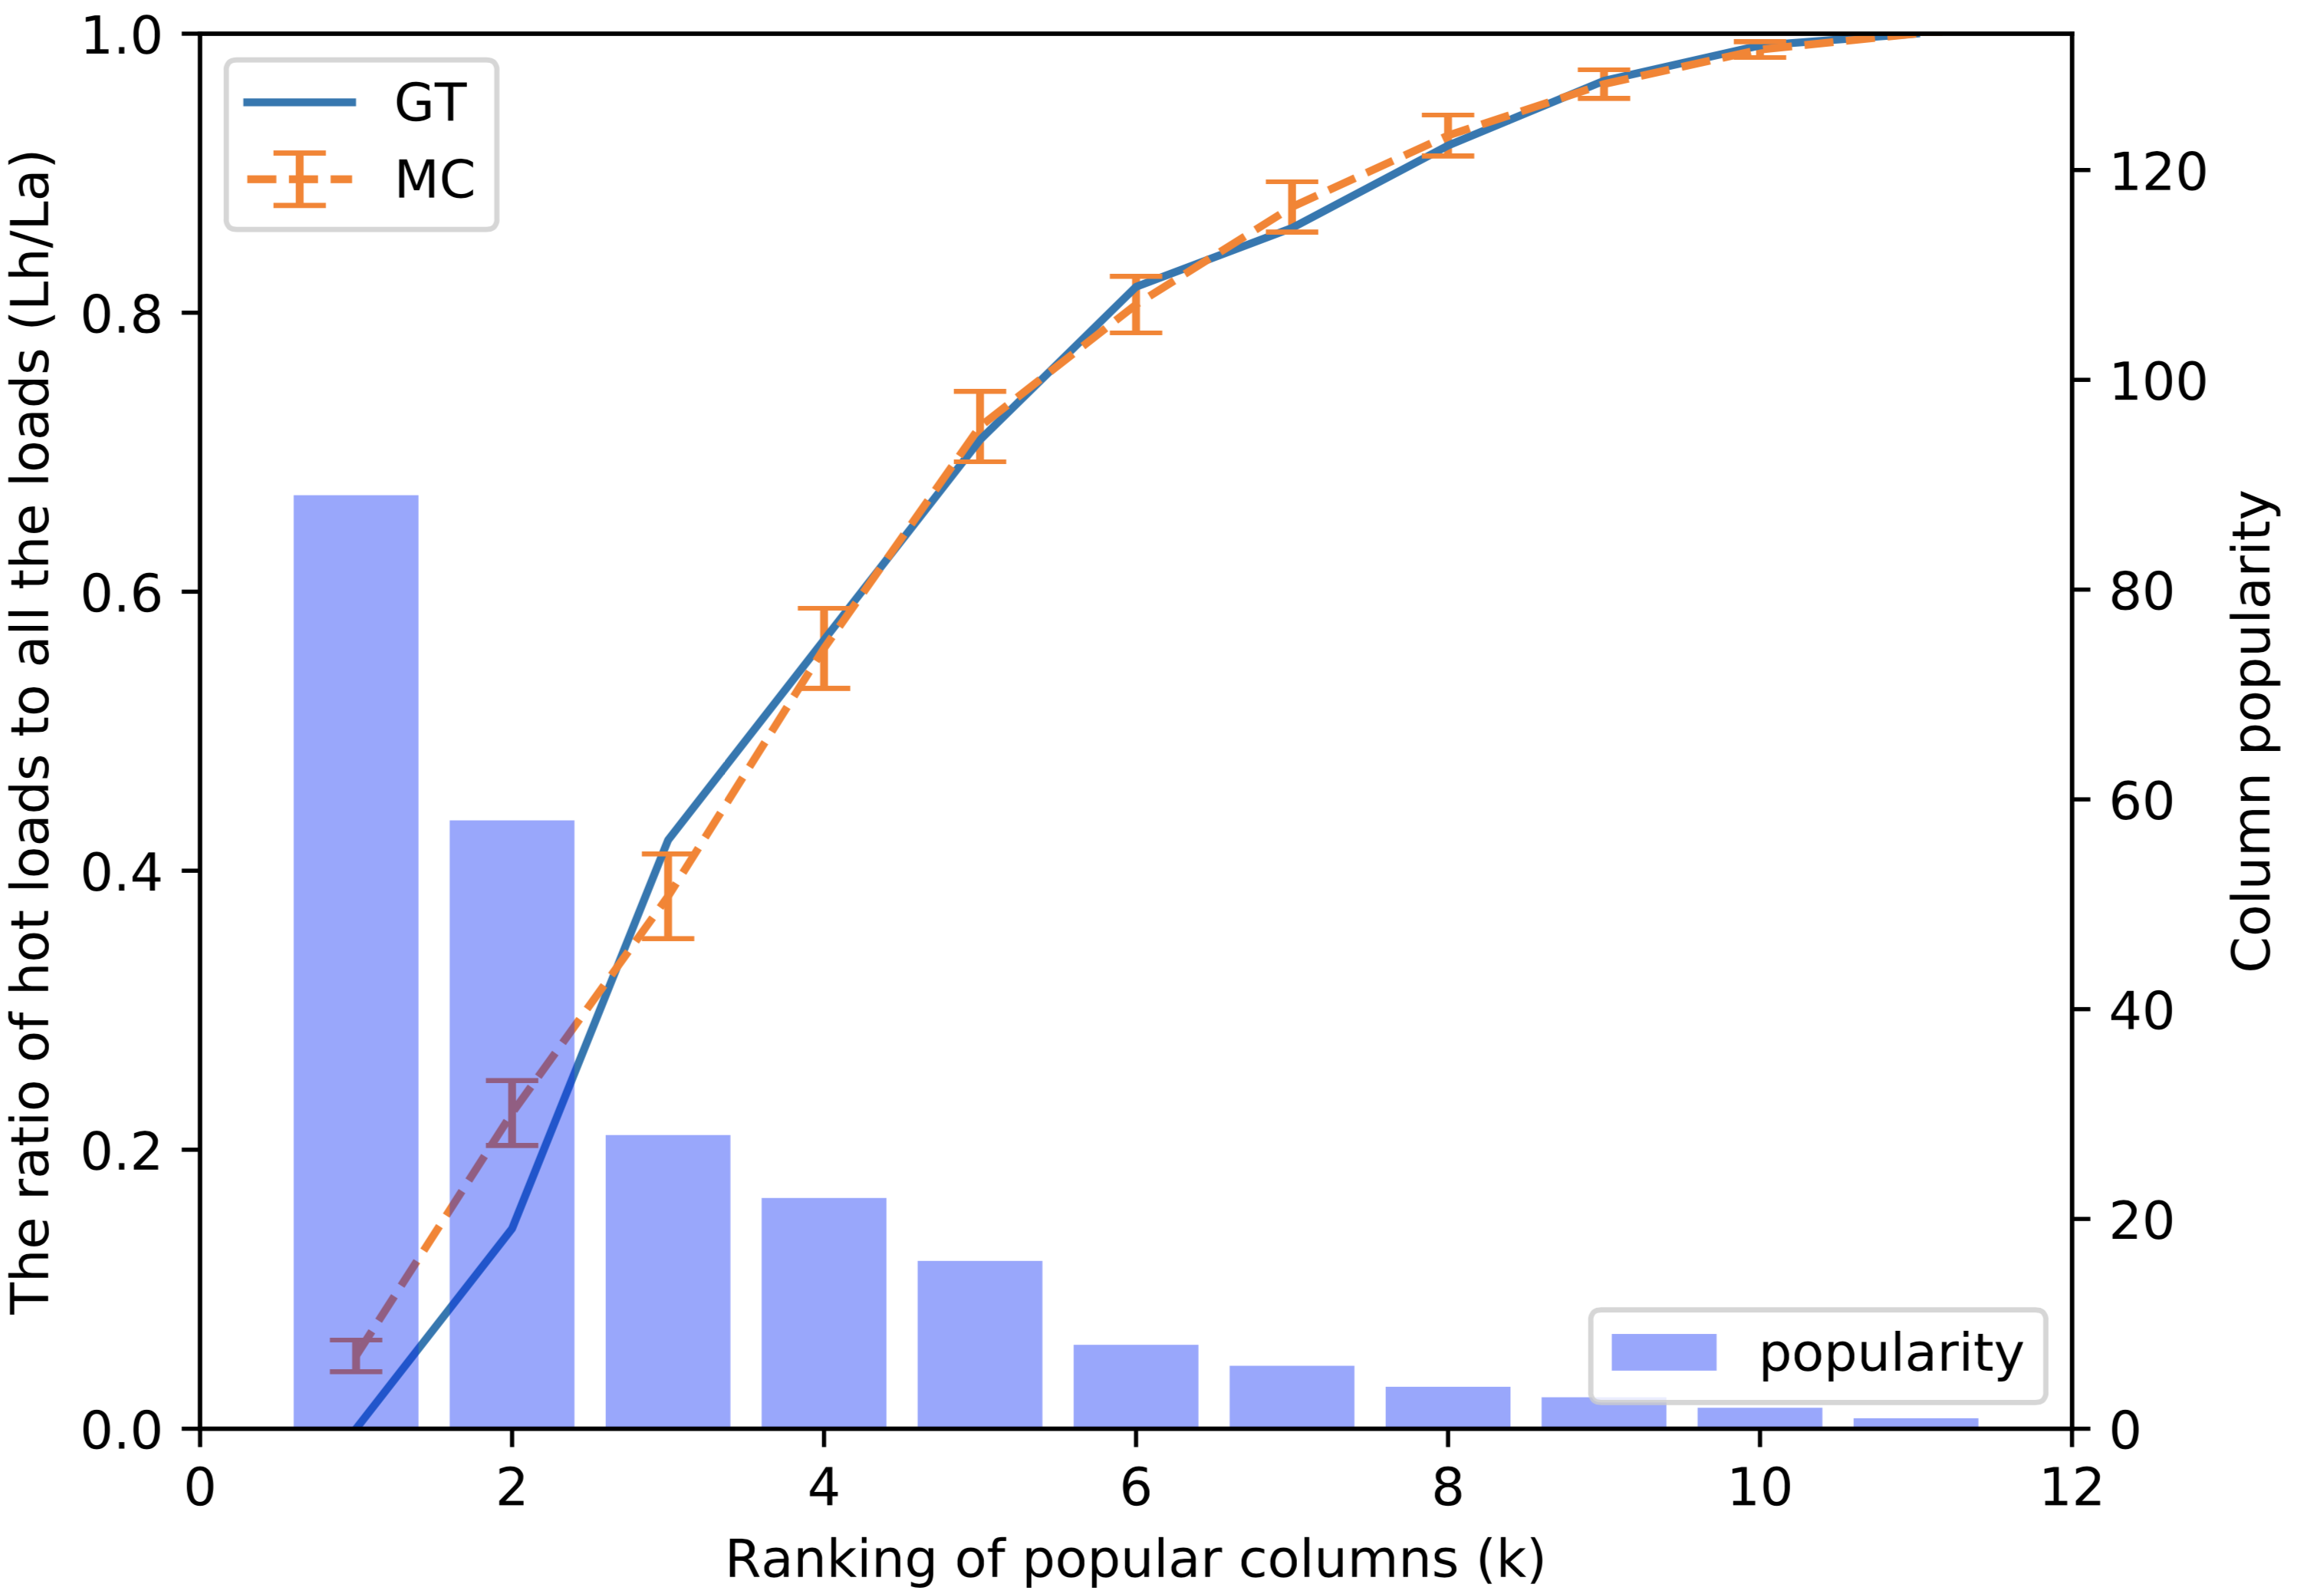
\includegraphics[width=1\textwidth]{img/cw-cache/ca_date_dim}
        \caption{TPC-DS中的 $data\_dim$ 表}
        \label{fig:ca-dd}
    \end{subfigure}%
    
    \begin{subfigure}[t]{0.5\textwidth}
        \centering
        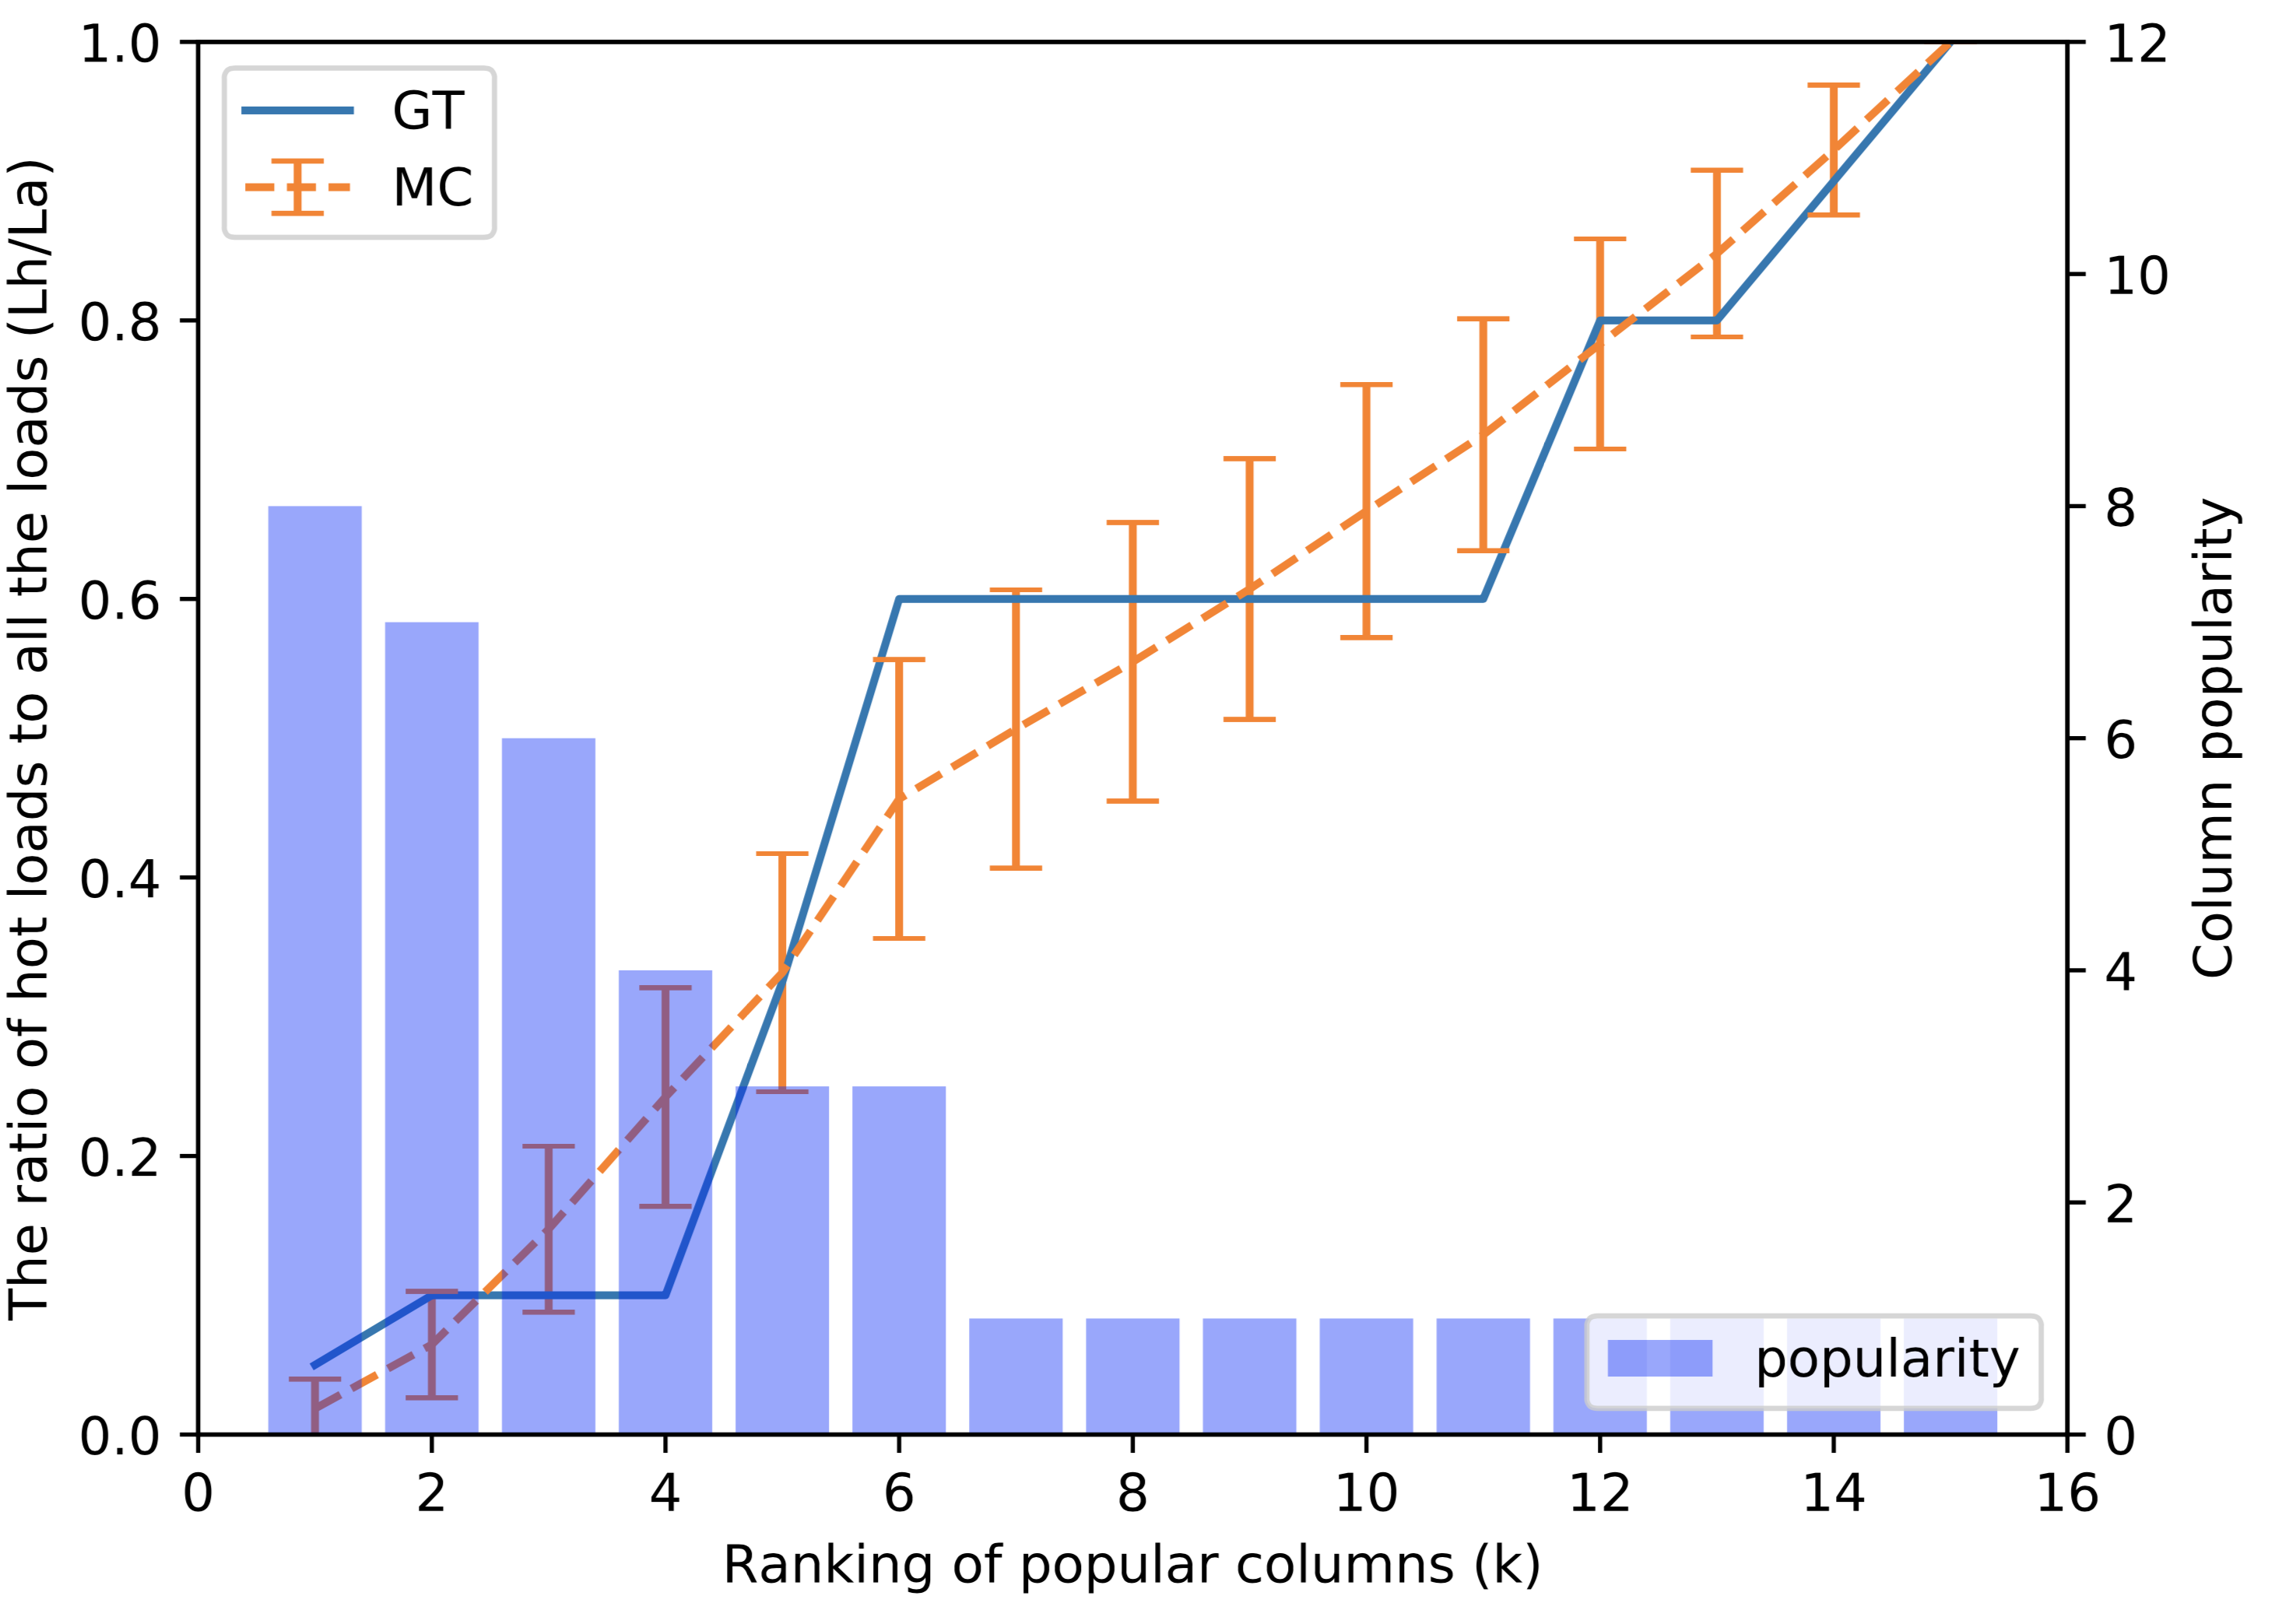
\includegraphics[width=1\textwidth]{img/cw-cache/ca_web_returns}
        \caption{TDC-DS中的 $web\_returns$ 表}
        \label{fig:ca-wr}
    \end{subfigure}%
    
    \begin{subfigure}[t]{0.5\textwidth}
        \centering
        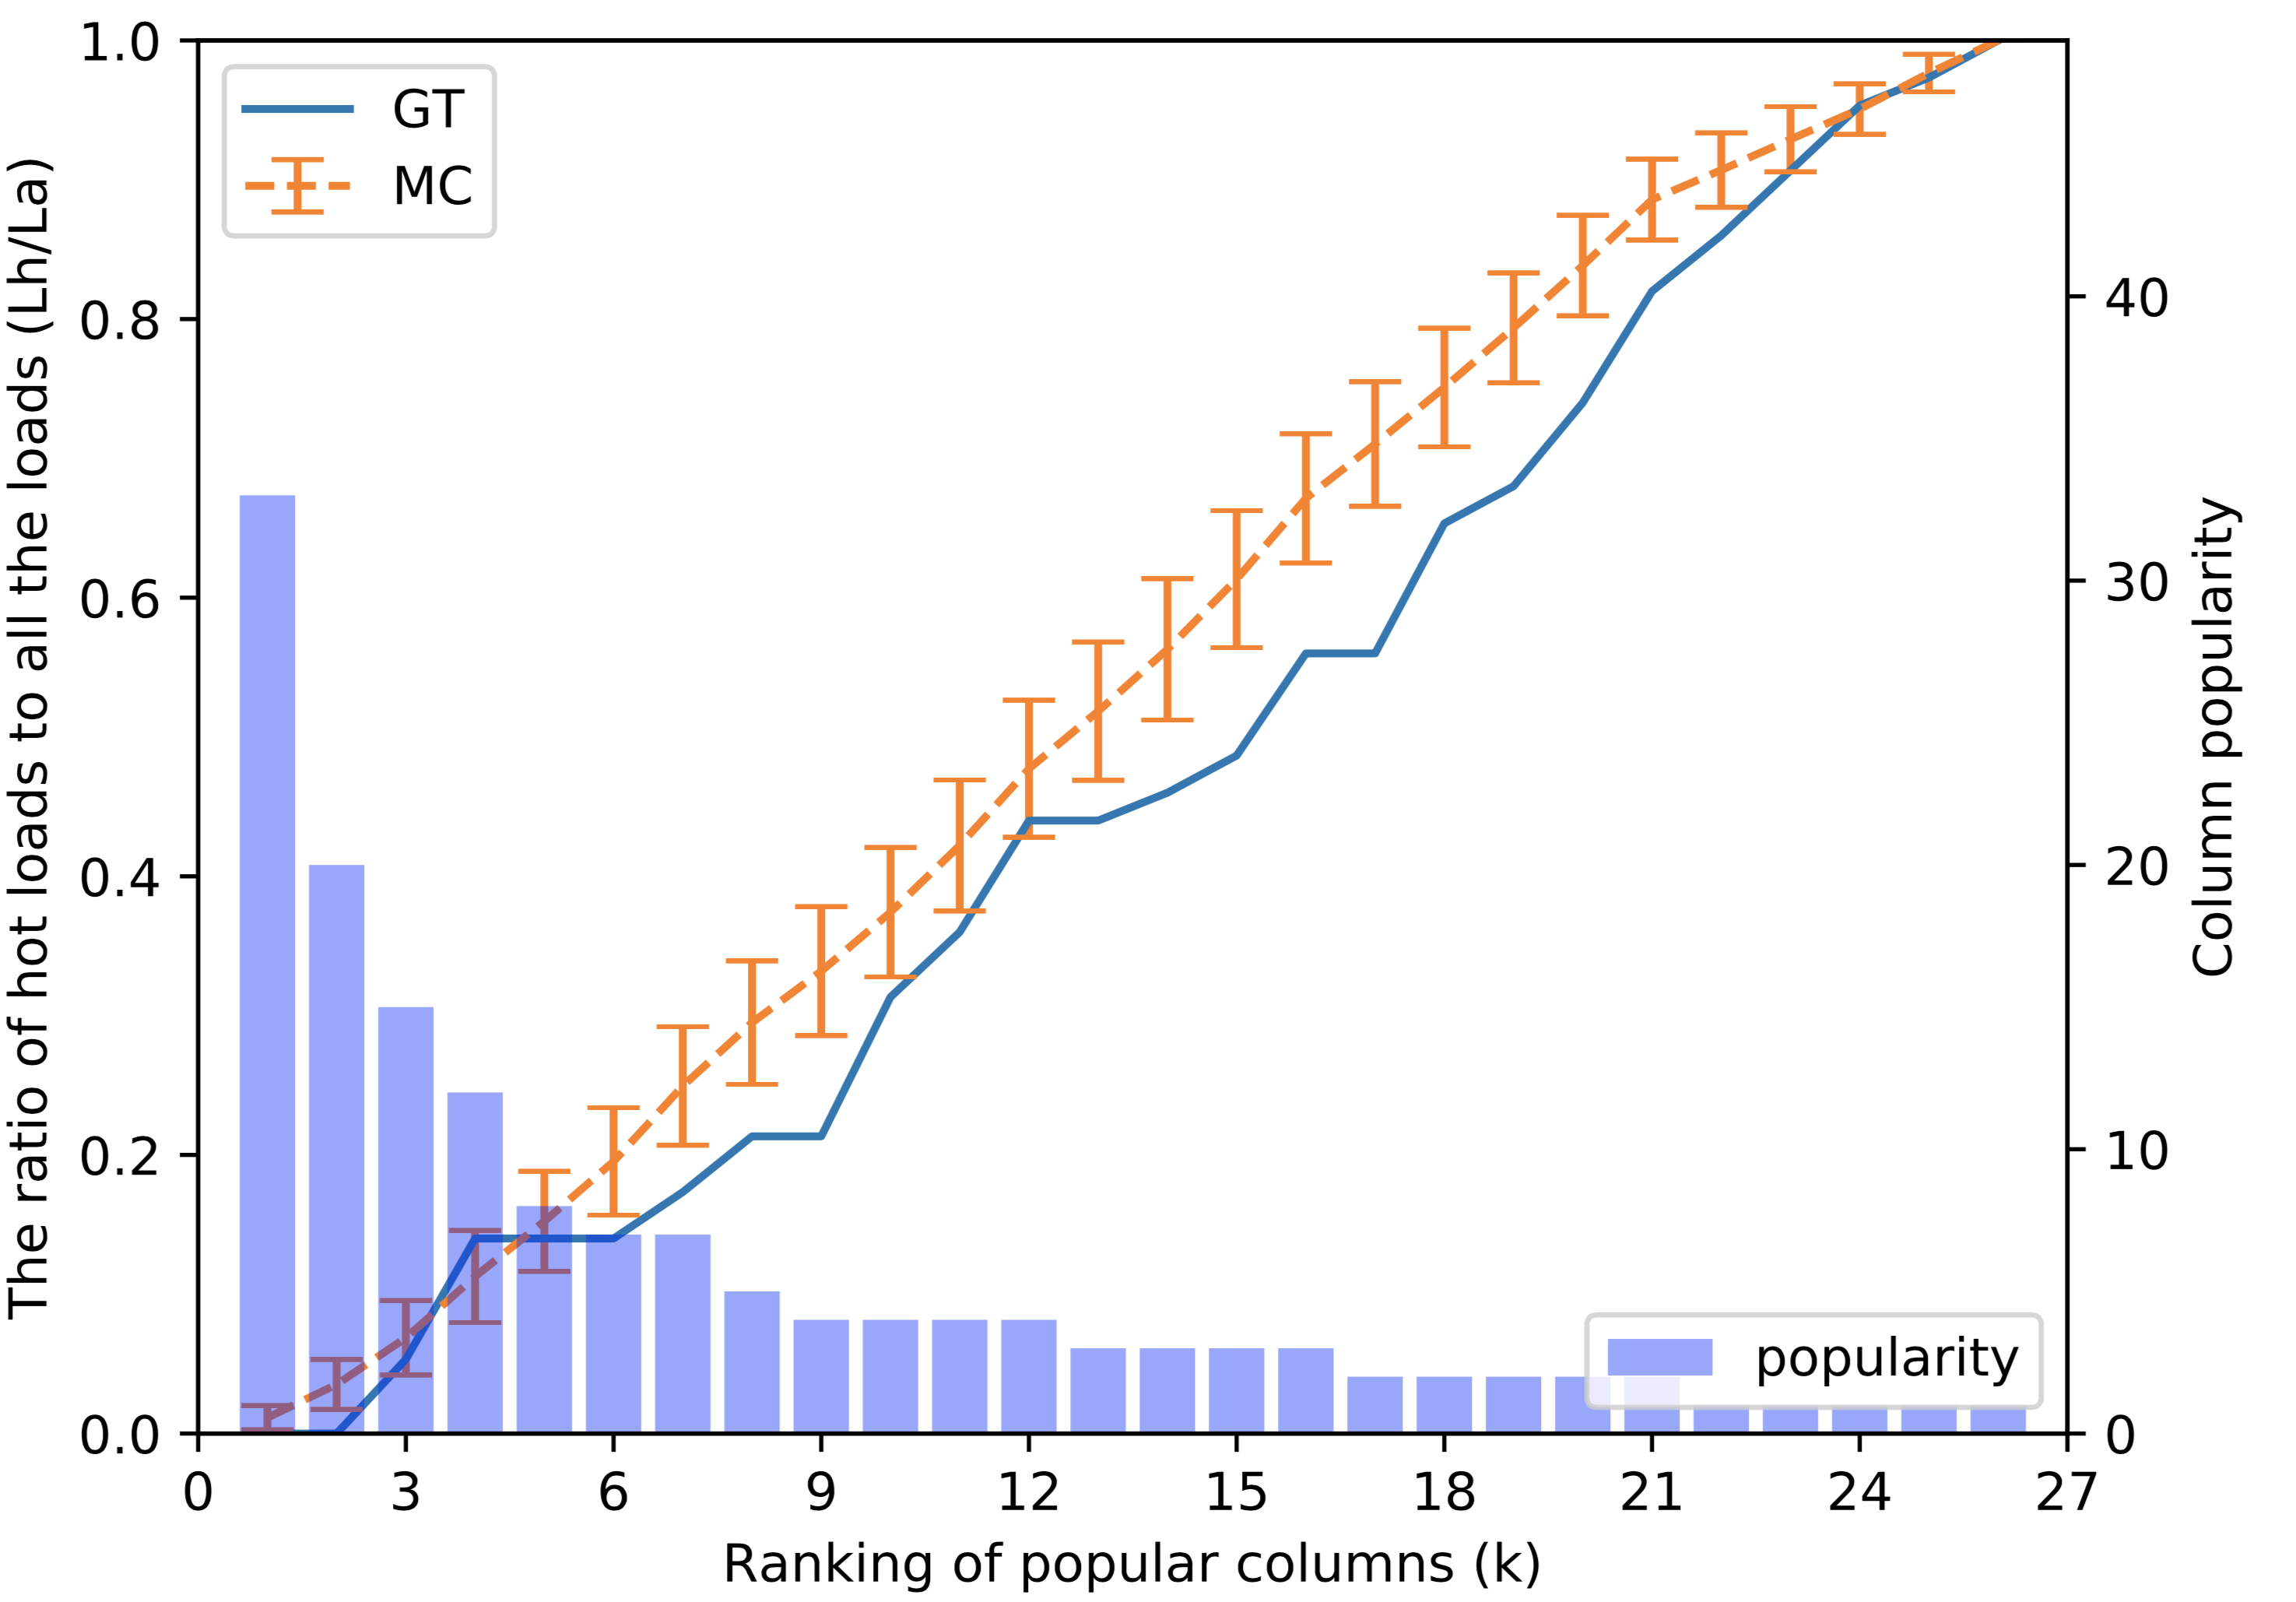
\includegraphics[width=1\textwidth]{img/cw-cache/ca_web_sales}
        \caption{TDC-DS中的 $web\_sales$ t表}
        \label{fig:ca-ws}
    \end{subfigure}%
    \caption{列的热度及归一化的$L_h$ 和 $k$之间的关系。蒙特卡罗方法 vs. 实际情况(Ground Truth)}
    \label{fig:mc_gt}
    %\vspace{-.1in}
\end{figure}
 
\par \noindent\textbf{分析} 为分析这个方法,我们简单地假设共有$m$个查询任务,每一个有 $B = \left\{\frac{p_{1}}{m}, \frac{p_{2}}{m}, \dots, \frac{p_{n}}{m}\right\}$ 的概率访问 $n$ 个列。我们的目标是给定 $k$,估算 $L_h$。

\par 考虑一个特定的查询任务 $q_i$,给定 $k$ 值,记$X_i$为一个二元随机变量,表示$q_i$涉及 的列能否被前$k$个最热门的列覆盖。我们有:
\begin{equation}
\Pr\left[X_{i}=1\right]=\prod_{i=k+1}^{n}\left(1-\frac{p_{i}}{m}\right)
\end{equation}

\par 假设来自查询任务$q_i$的负载是$d_i$,其中$d_i$是其访问的列的大小之和。如果$X_i =1$,那么$d_i$的期望值为:
\begin{equation}
E\left[d_i\right]=\sum_{i=1}^{k} \frac{p_{i} s_{i}}{m}=\frac{\sum_{i=1}^{k} l_{i}}{m}
\end{equation}

记$X$为可以由前$k$个最热门的列承担的查询任务的数量,则:
\begin{equation}
X = \sum_{i=1}^m X_i = m \prod_{i=k+1}^{n}\left(1-\frac{p_{i}}{m}\right)
\end{equation}

因此,对于$L_h$,我们有:
\begin{equation}
\label{equ:lh}
\begin{split}
L_h &= \frac{\sum_{i=1}^{k} l_{i}}{m}  \cdot m \prod_{i=k+1}^{n}\left(1-\frac{p_{i}}{m}\right) \\
&= \sum_{i=1}^{k} l_{i} \prod_{i=k+1}^{n}\left(1-\frac{p_{i}}{m}\right)
\end{split}
\end{equation}

根据等式~\ref{equ:lh},当各个列的负载差异程度很高(highly skewed)的时候,当$k$值较小时,$L_h$随着$k$的增大迅速增大。

\par \noindent \textbf{测量实验2} 我们做实验对比了用等式~\ref{equ:lh}求得的$L_h$的预测值(PV)和通过蒙特卡罗方法得到的$L_h$的值,结果展示在图~\ref{fig:mc_pv} 中,可以看到,两条曲线表现出相似的趋势。我们注意到这两种方法求出的$L_h$的值有误差,原因是我们假设了生成的查询任务是相互独立的,然而这些生成的查询任务包含的列不能超出各个列的定额,这导致在查询任务生成过程后期产生的那些任务实际是有依赖关系的,具体来说,当列 $c_i$的定额用尽,那么后面生成的查询任务访问列$c_i$的概率是$0$而不是$\frac{p_i}{m}$。在实际操作中,我们需要生成的查询任务的数量超出$m$,以便消耗所有列的定额。

\par 事实上,当生成的查询任务的数量变得很大时,公式预测的$L_h$的值能够接近蒙特卡罗方法得到的值。


\begin{figure}[]
    \centering
    \begin{minipage}[t]{0.5\textwidth}
        \begin{subfigure}[t]{1\textwidth}
            \centering
            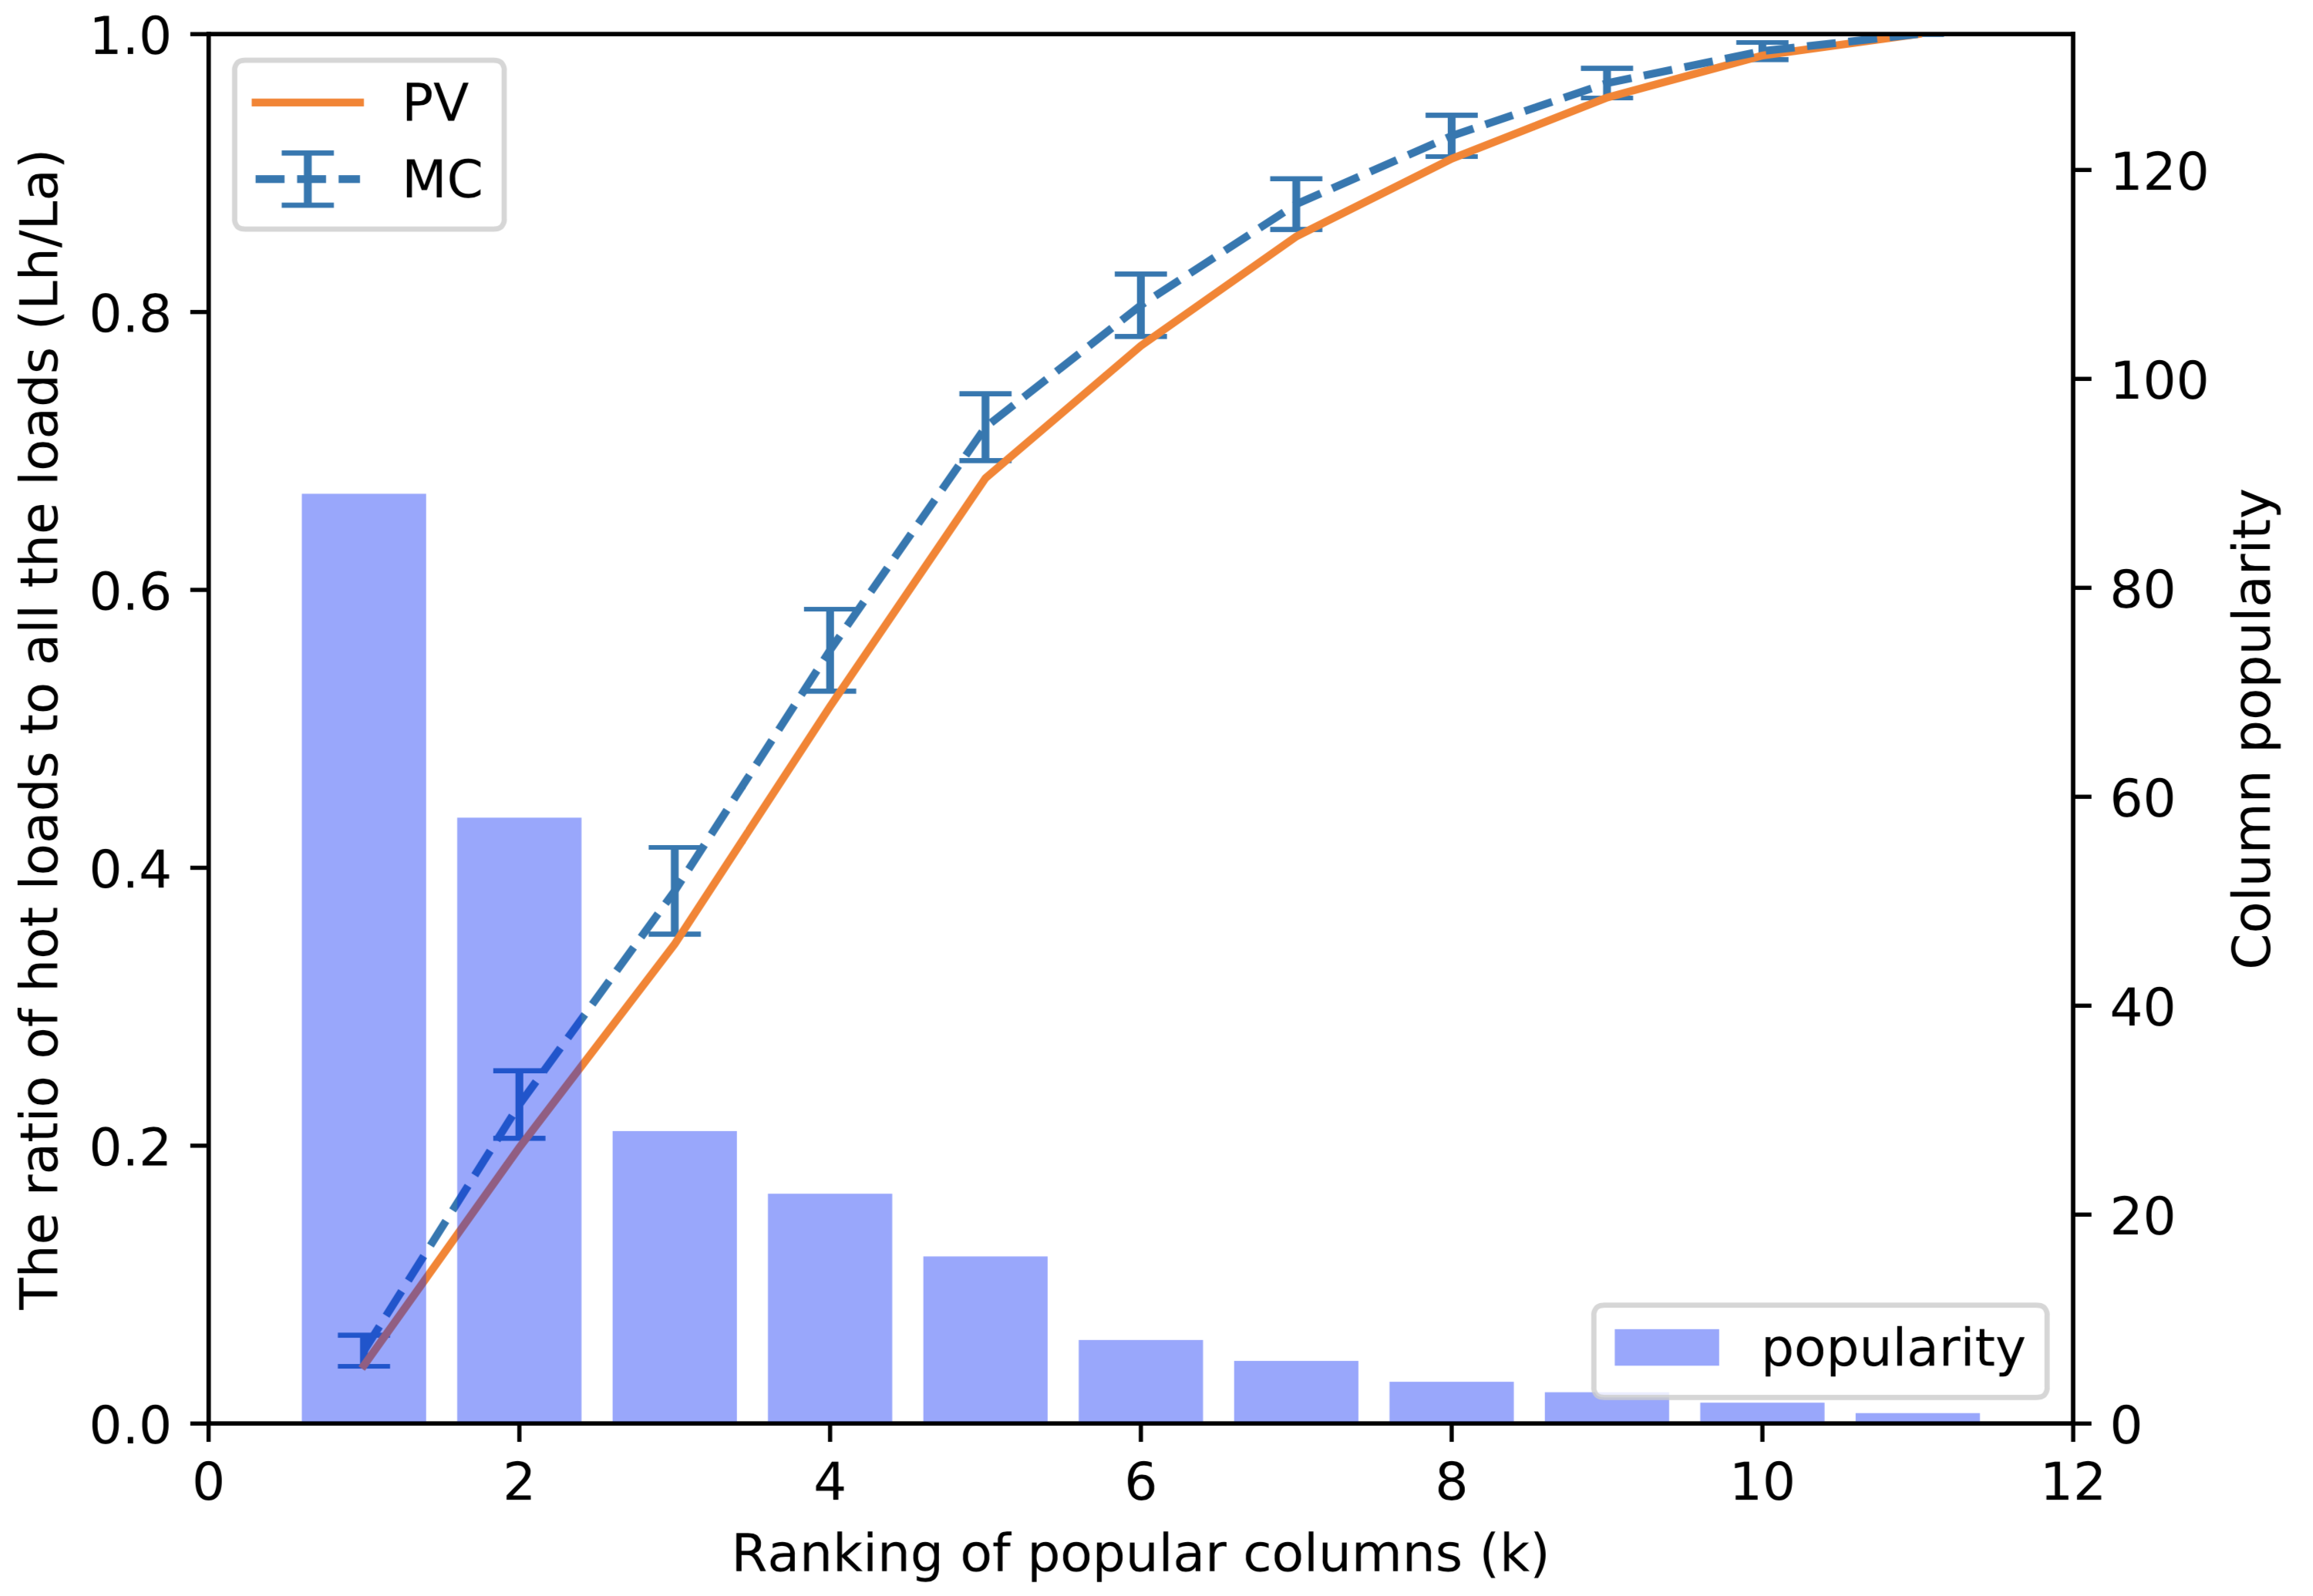
\includegraphics[width=1\textwidth]{img/cw-cache/calc_date_dim}
            \caption{TDC-DS中的 $data\_dim$ 表。}
            \label{fig:calc-dd}
        \end{subfigure}%

        \begin{subfigure}[t]{1\textwidth}
            \centering
            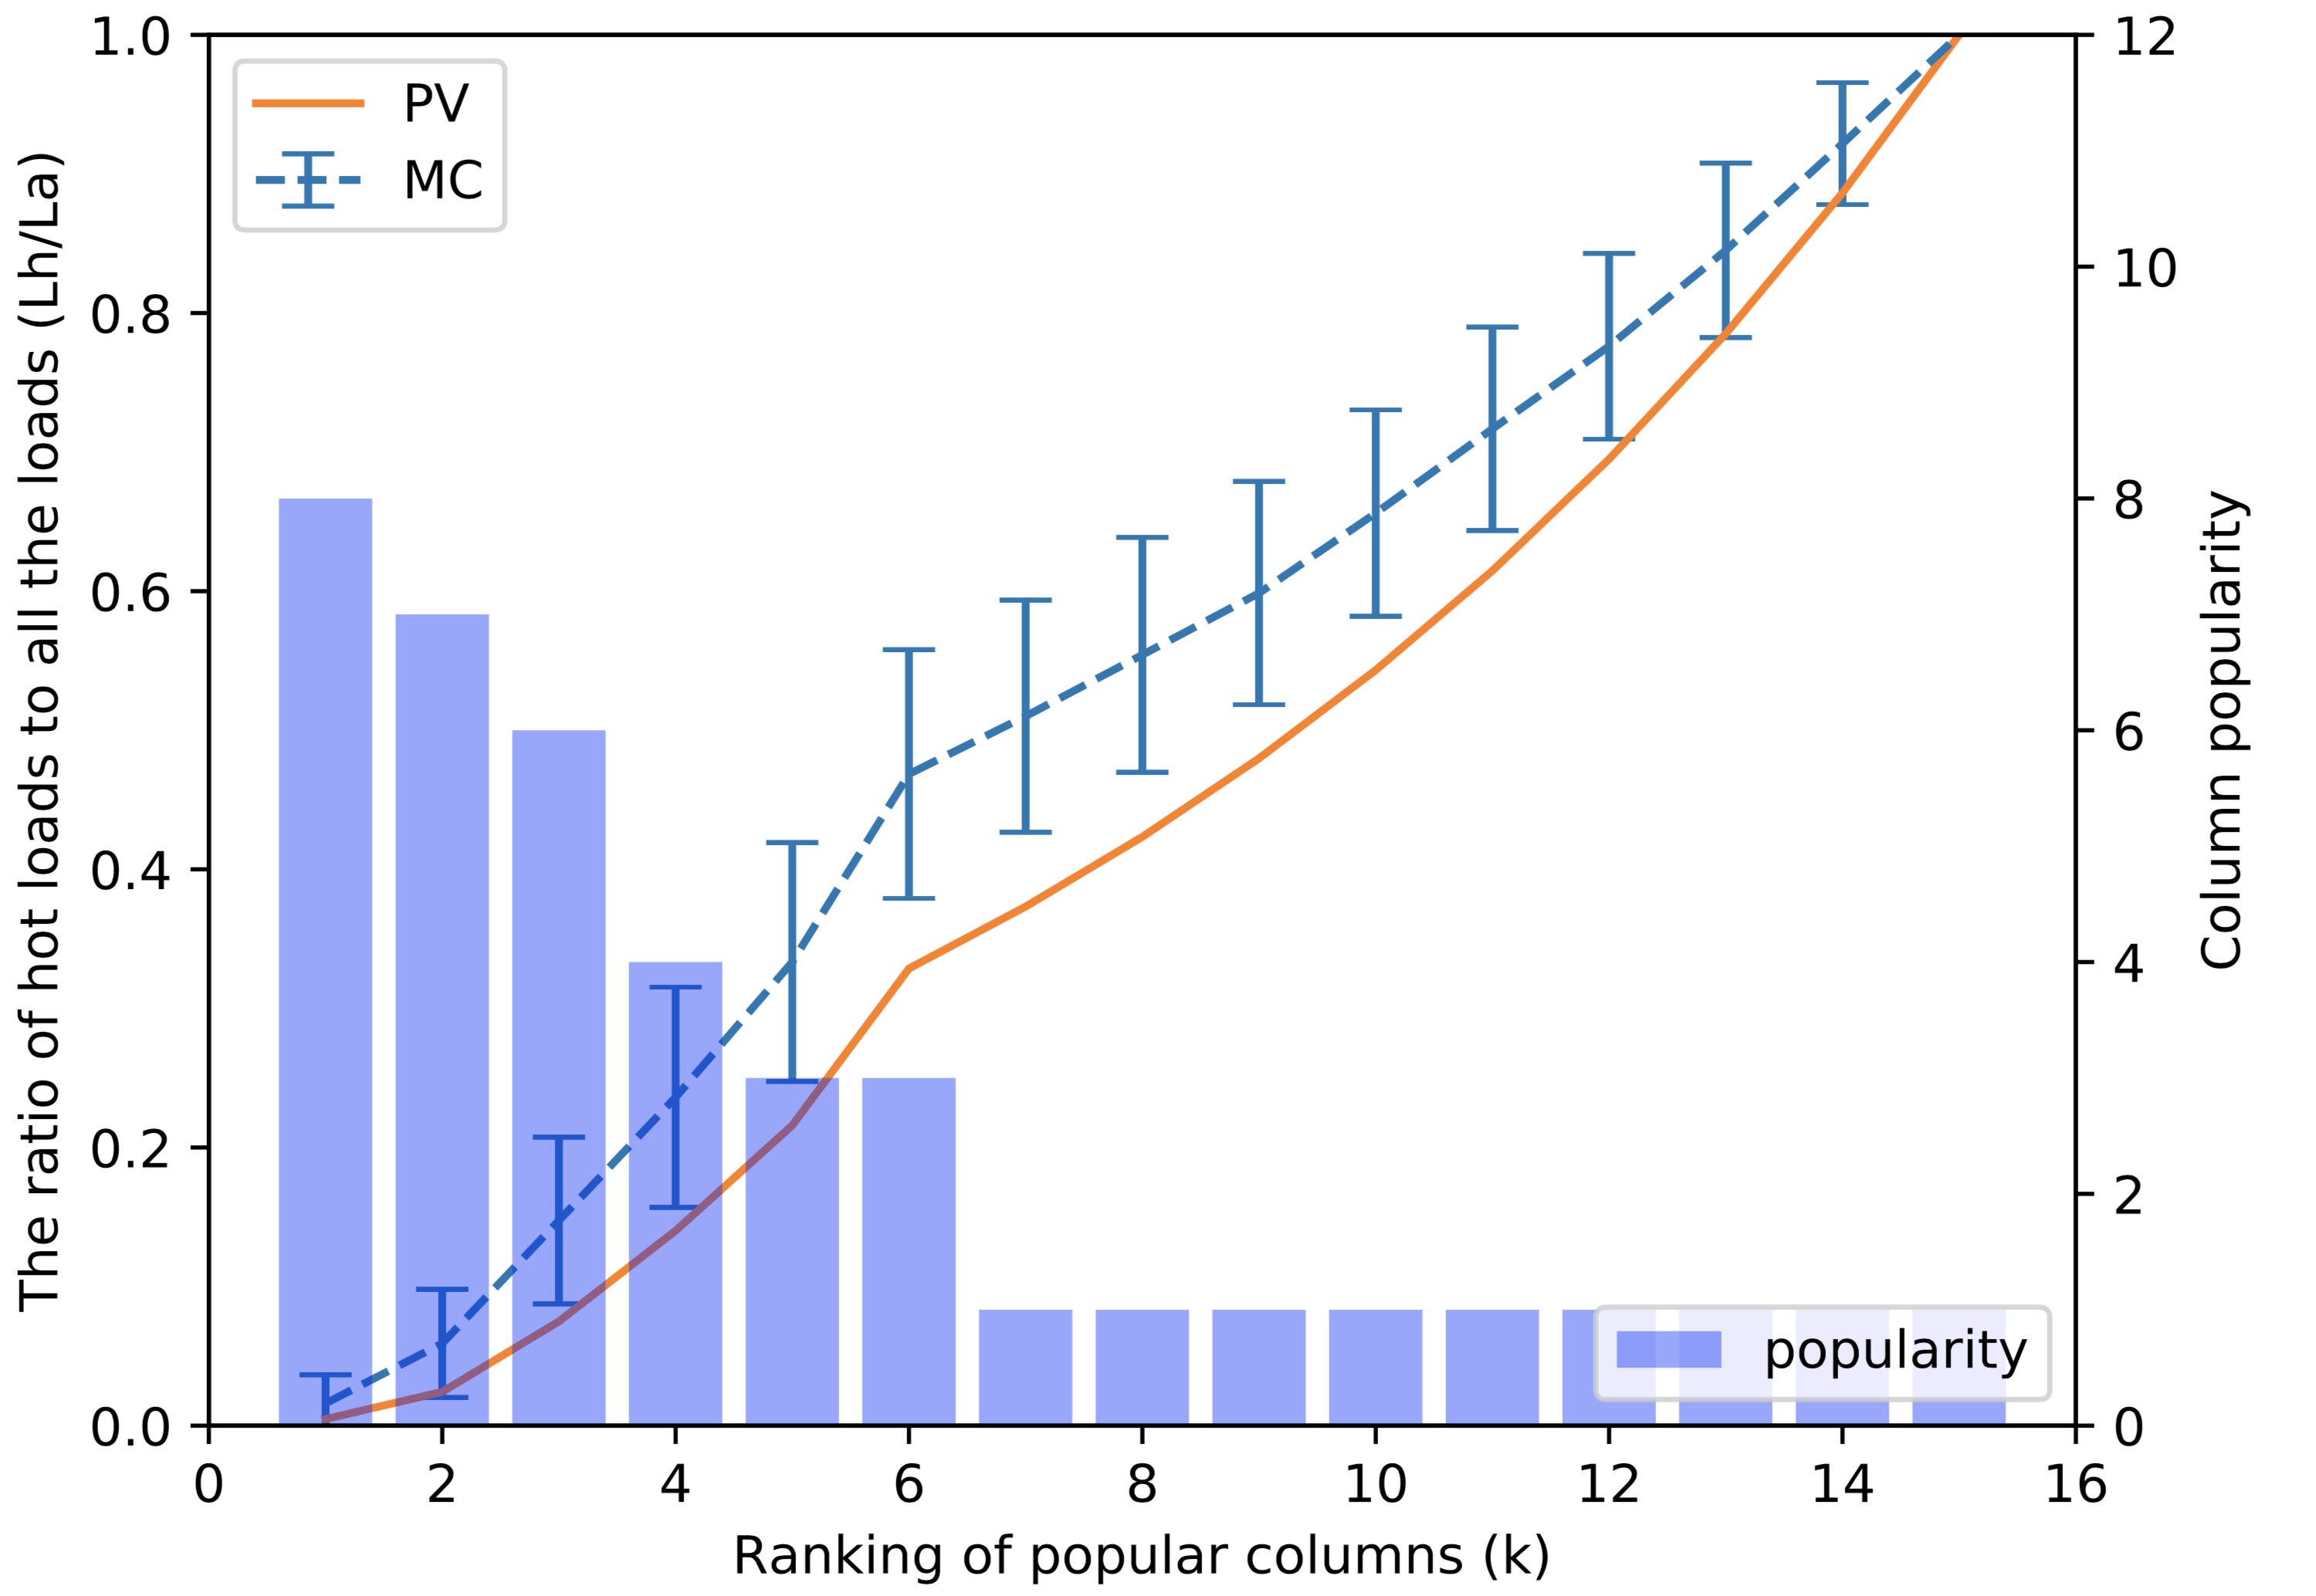
\includegraphics[width=1\textwidth]{img/cw-cache/calc_web_returns}
            \caption{TDC-DS中的 $web\_returns$ t表。}
            \label{fig:calc-wr}
        \end{subfigure}%

        \begin{subfigure}[t]{1\textwidth}
            \centering
            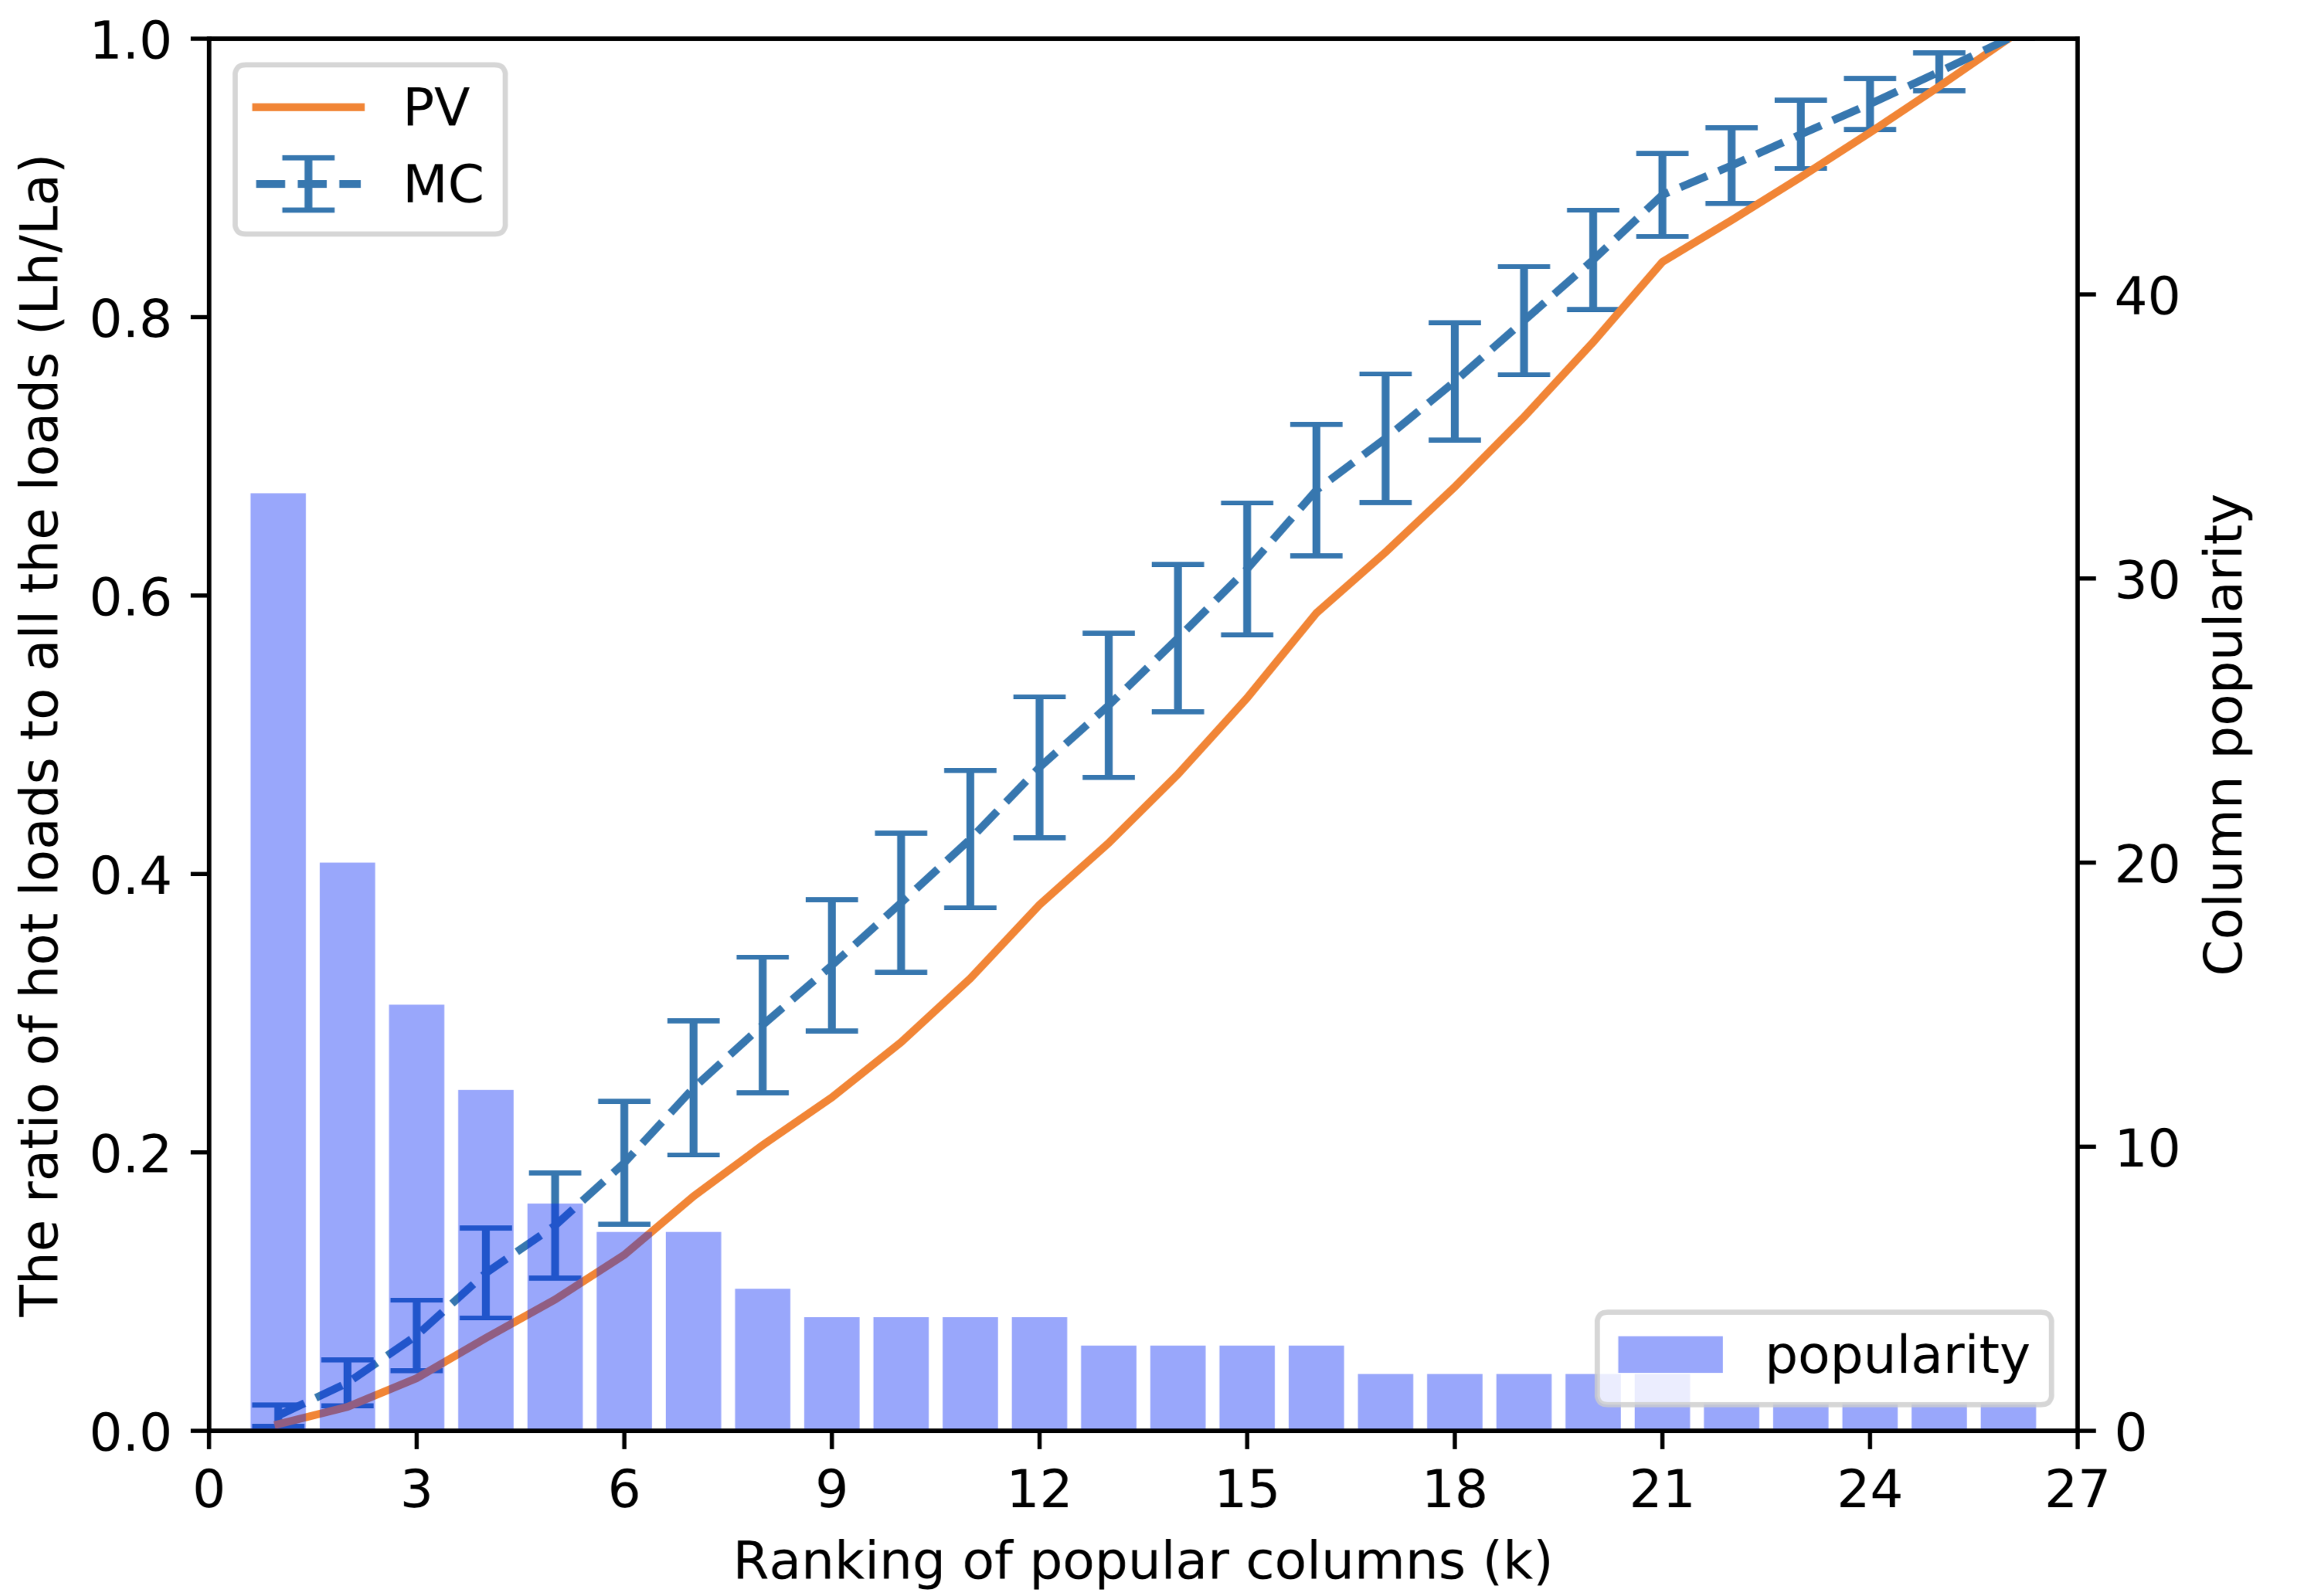
\includegraphics[width=1\textwidth]{img/cw-cache/calc_web_sales}
            \caption{TDC-DS中的 $web\_sales$ 表。}
            \label{fig:calc-ws}
        \end{subfigure}%
        \caption{列的热度及归一化的$L_h$ 和 $k$之间的关系。蒙特卡罗方法 vs. 公式预测}
	    \label{fig:mc_pv}
	    %\vspace{-.1in}
    \end{minipage}%
	\begin{minipage}[t]{0.5\textwidth}
        \centering
        \begin{subfigure}[t]{1\textwidth}
            \centering
            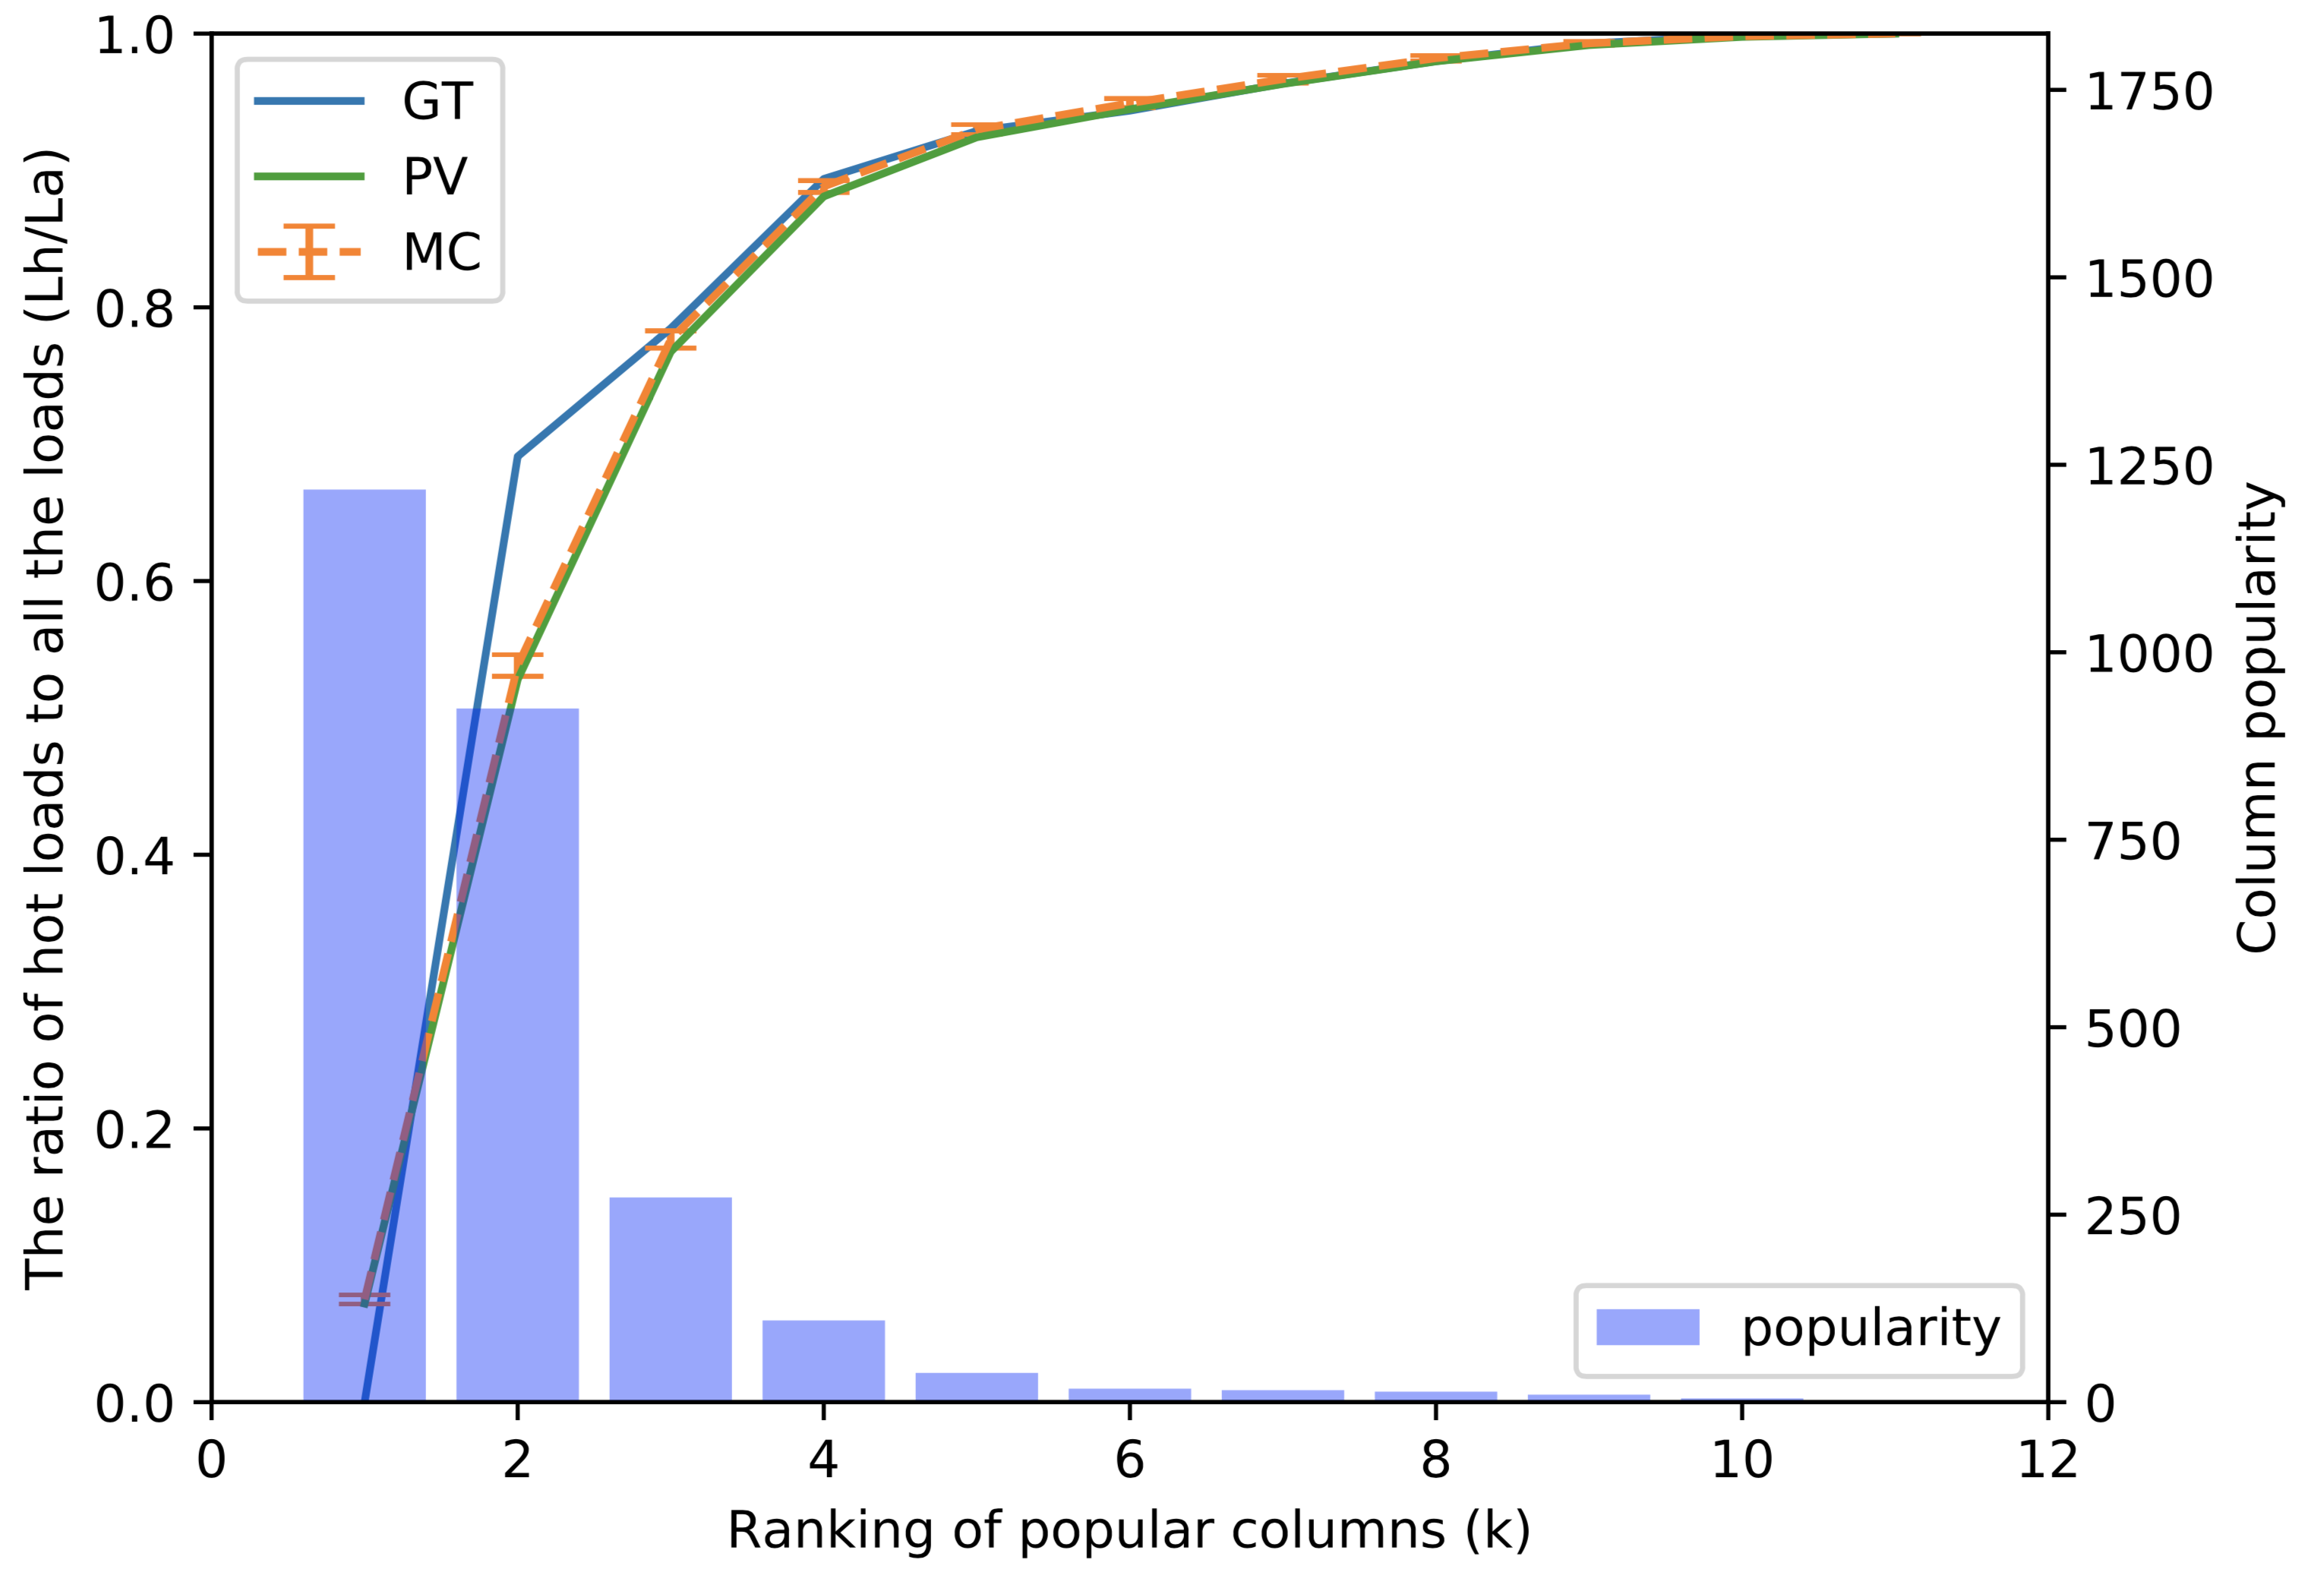
\includegraphics[width=1\textwidth]{img/cw-cache/emul_date_dim}
            \caption{TPC-DS中 $data\_dim$ 表。}
            \label{fig:emul-dd}
        \end{subfigure}%
        
        \begin{subfigure}[t]{1\textwidth}
            \centering
            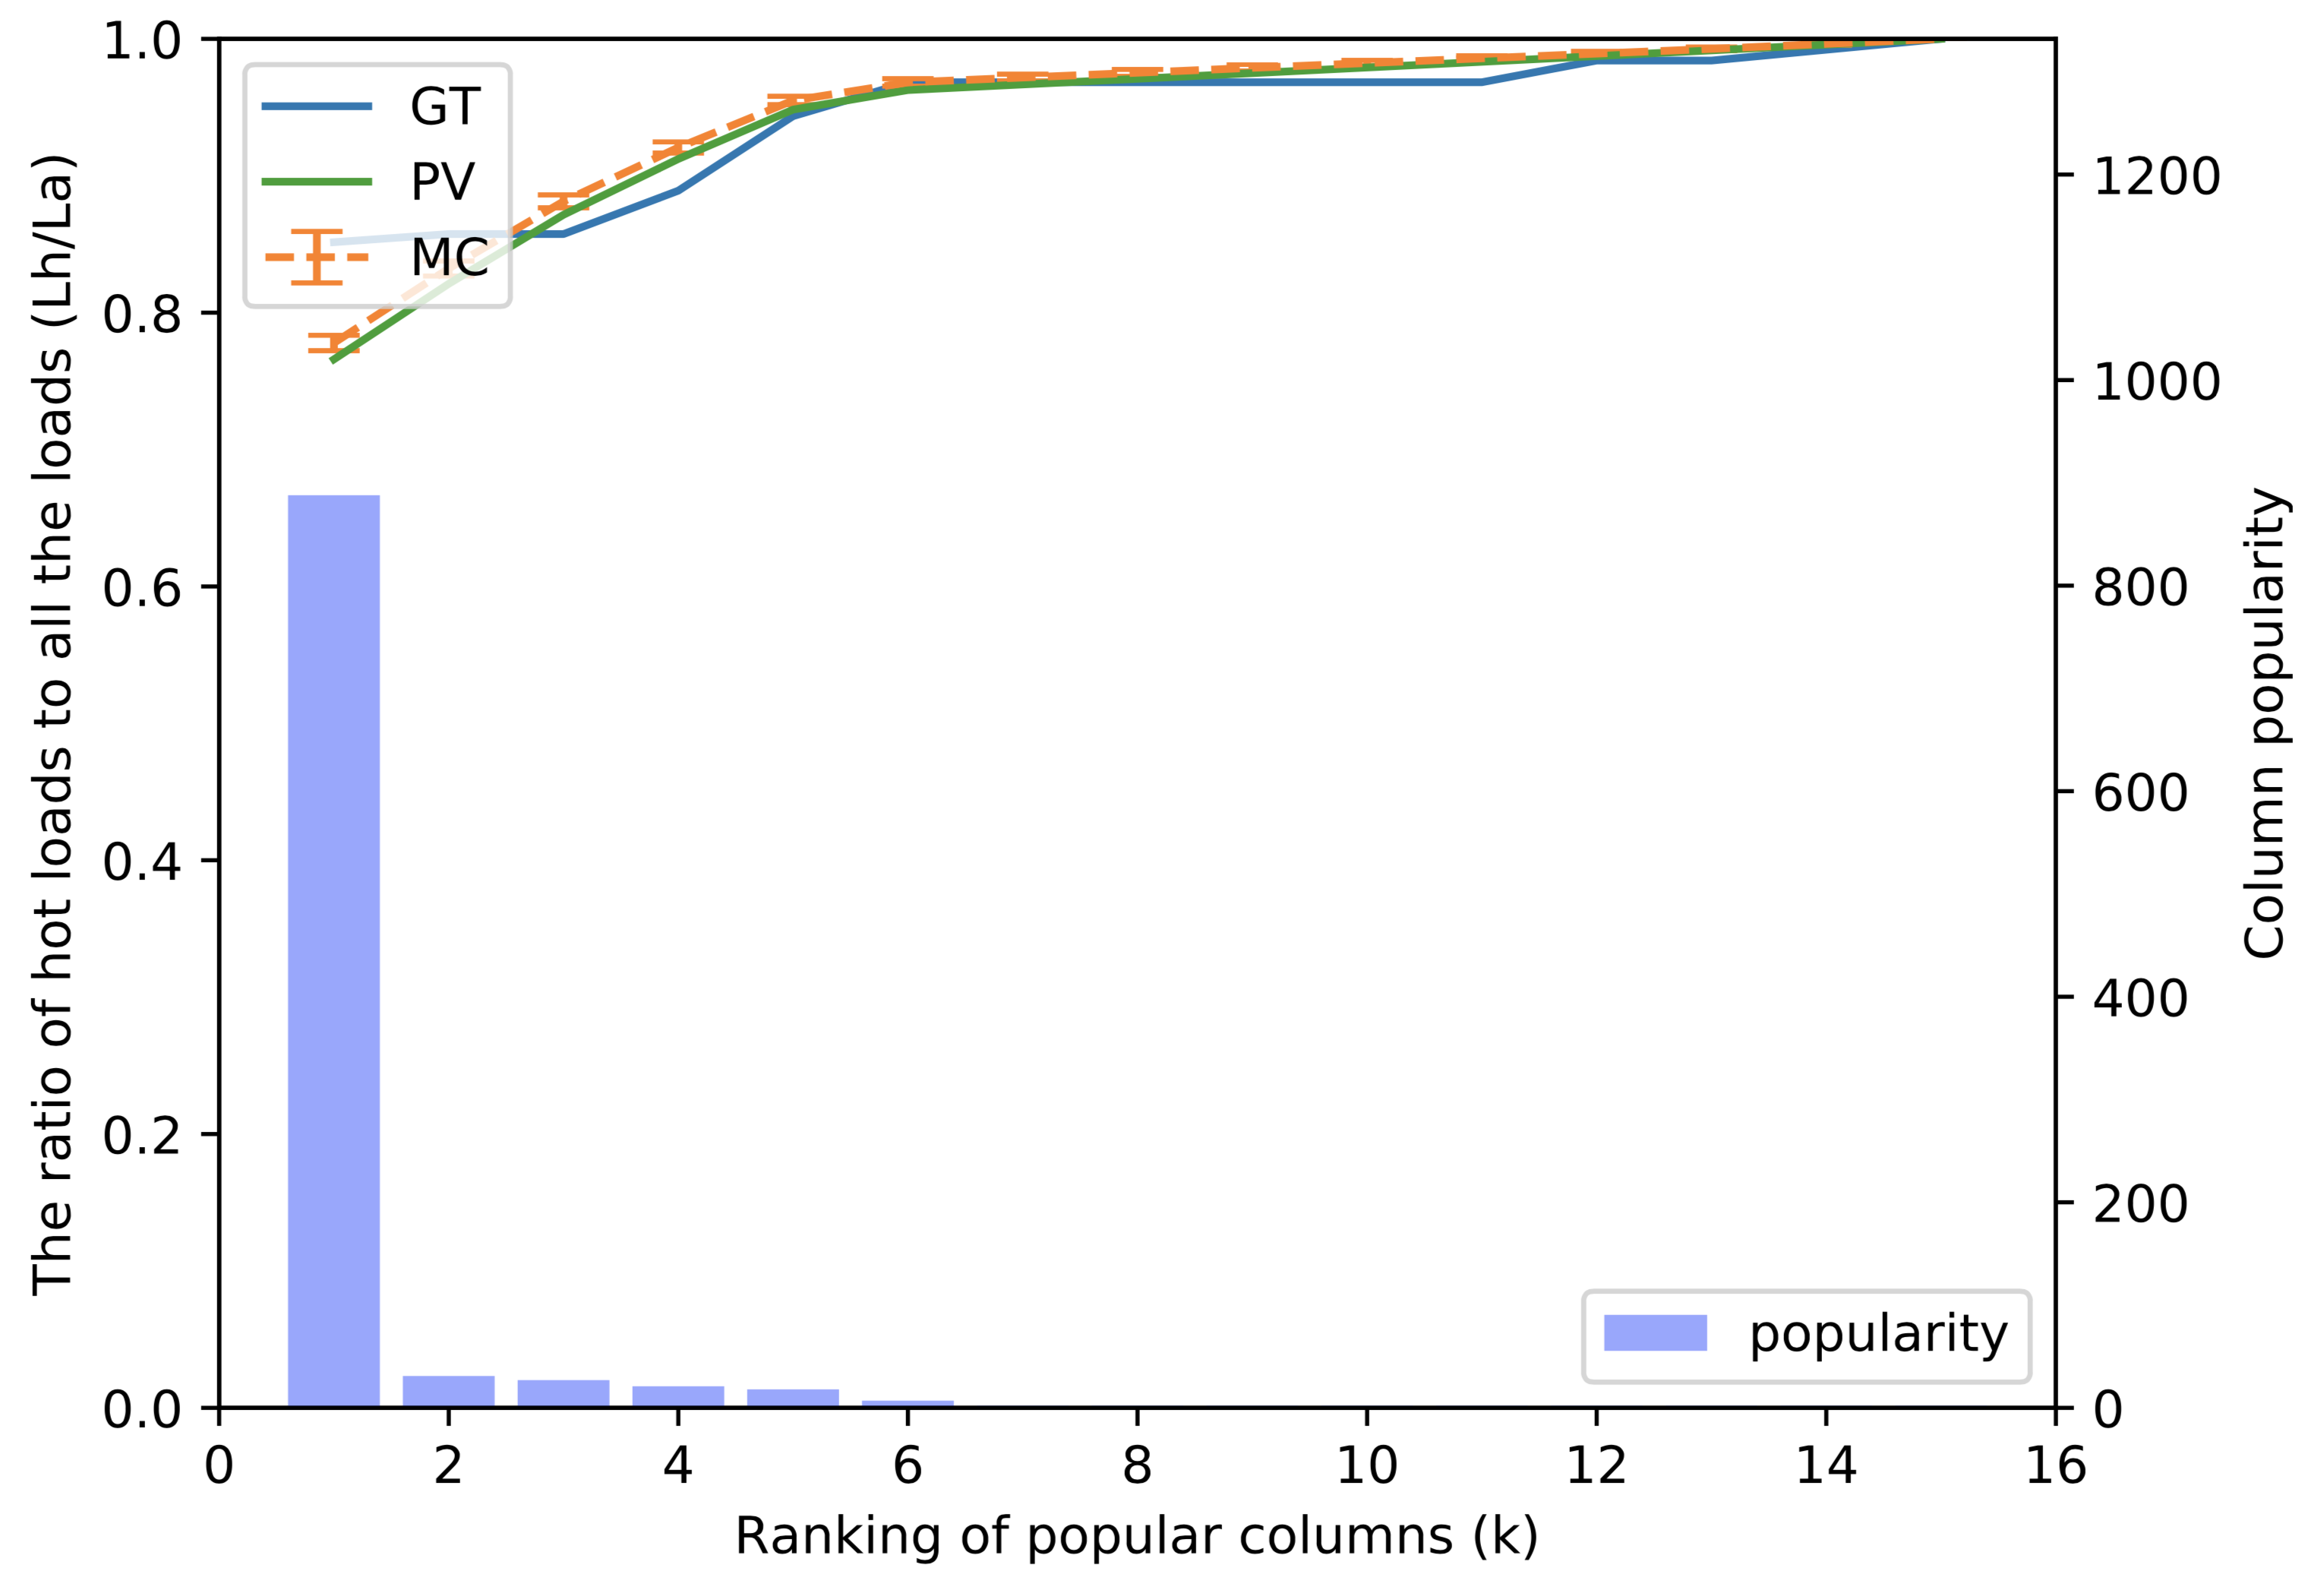
\includegraphics[width=1\textwidth]{img/cw-cache/emul_web_returns}
            \caption{TPC-DS中的 $web\_returns$ 表。}
            \label{fig:emul-wr}
        \end{subfigure}%
        
        \begin{subfigure}[t]{1\textwidth}
            \centering
            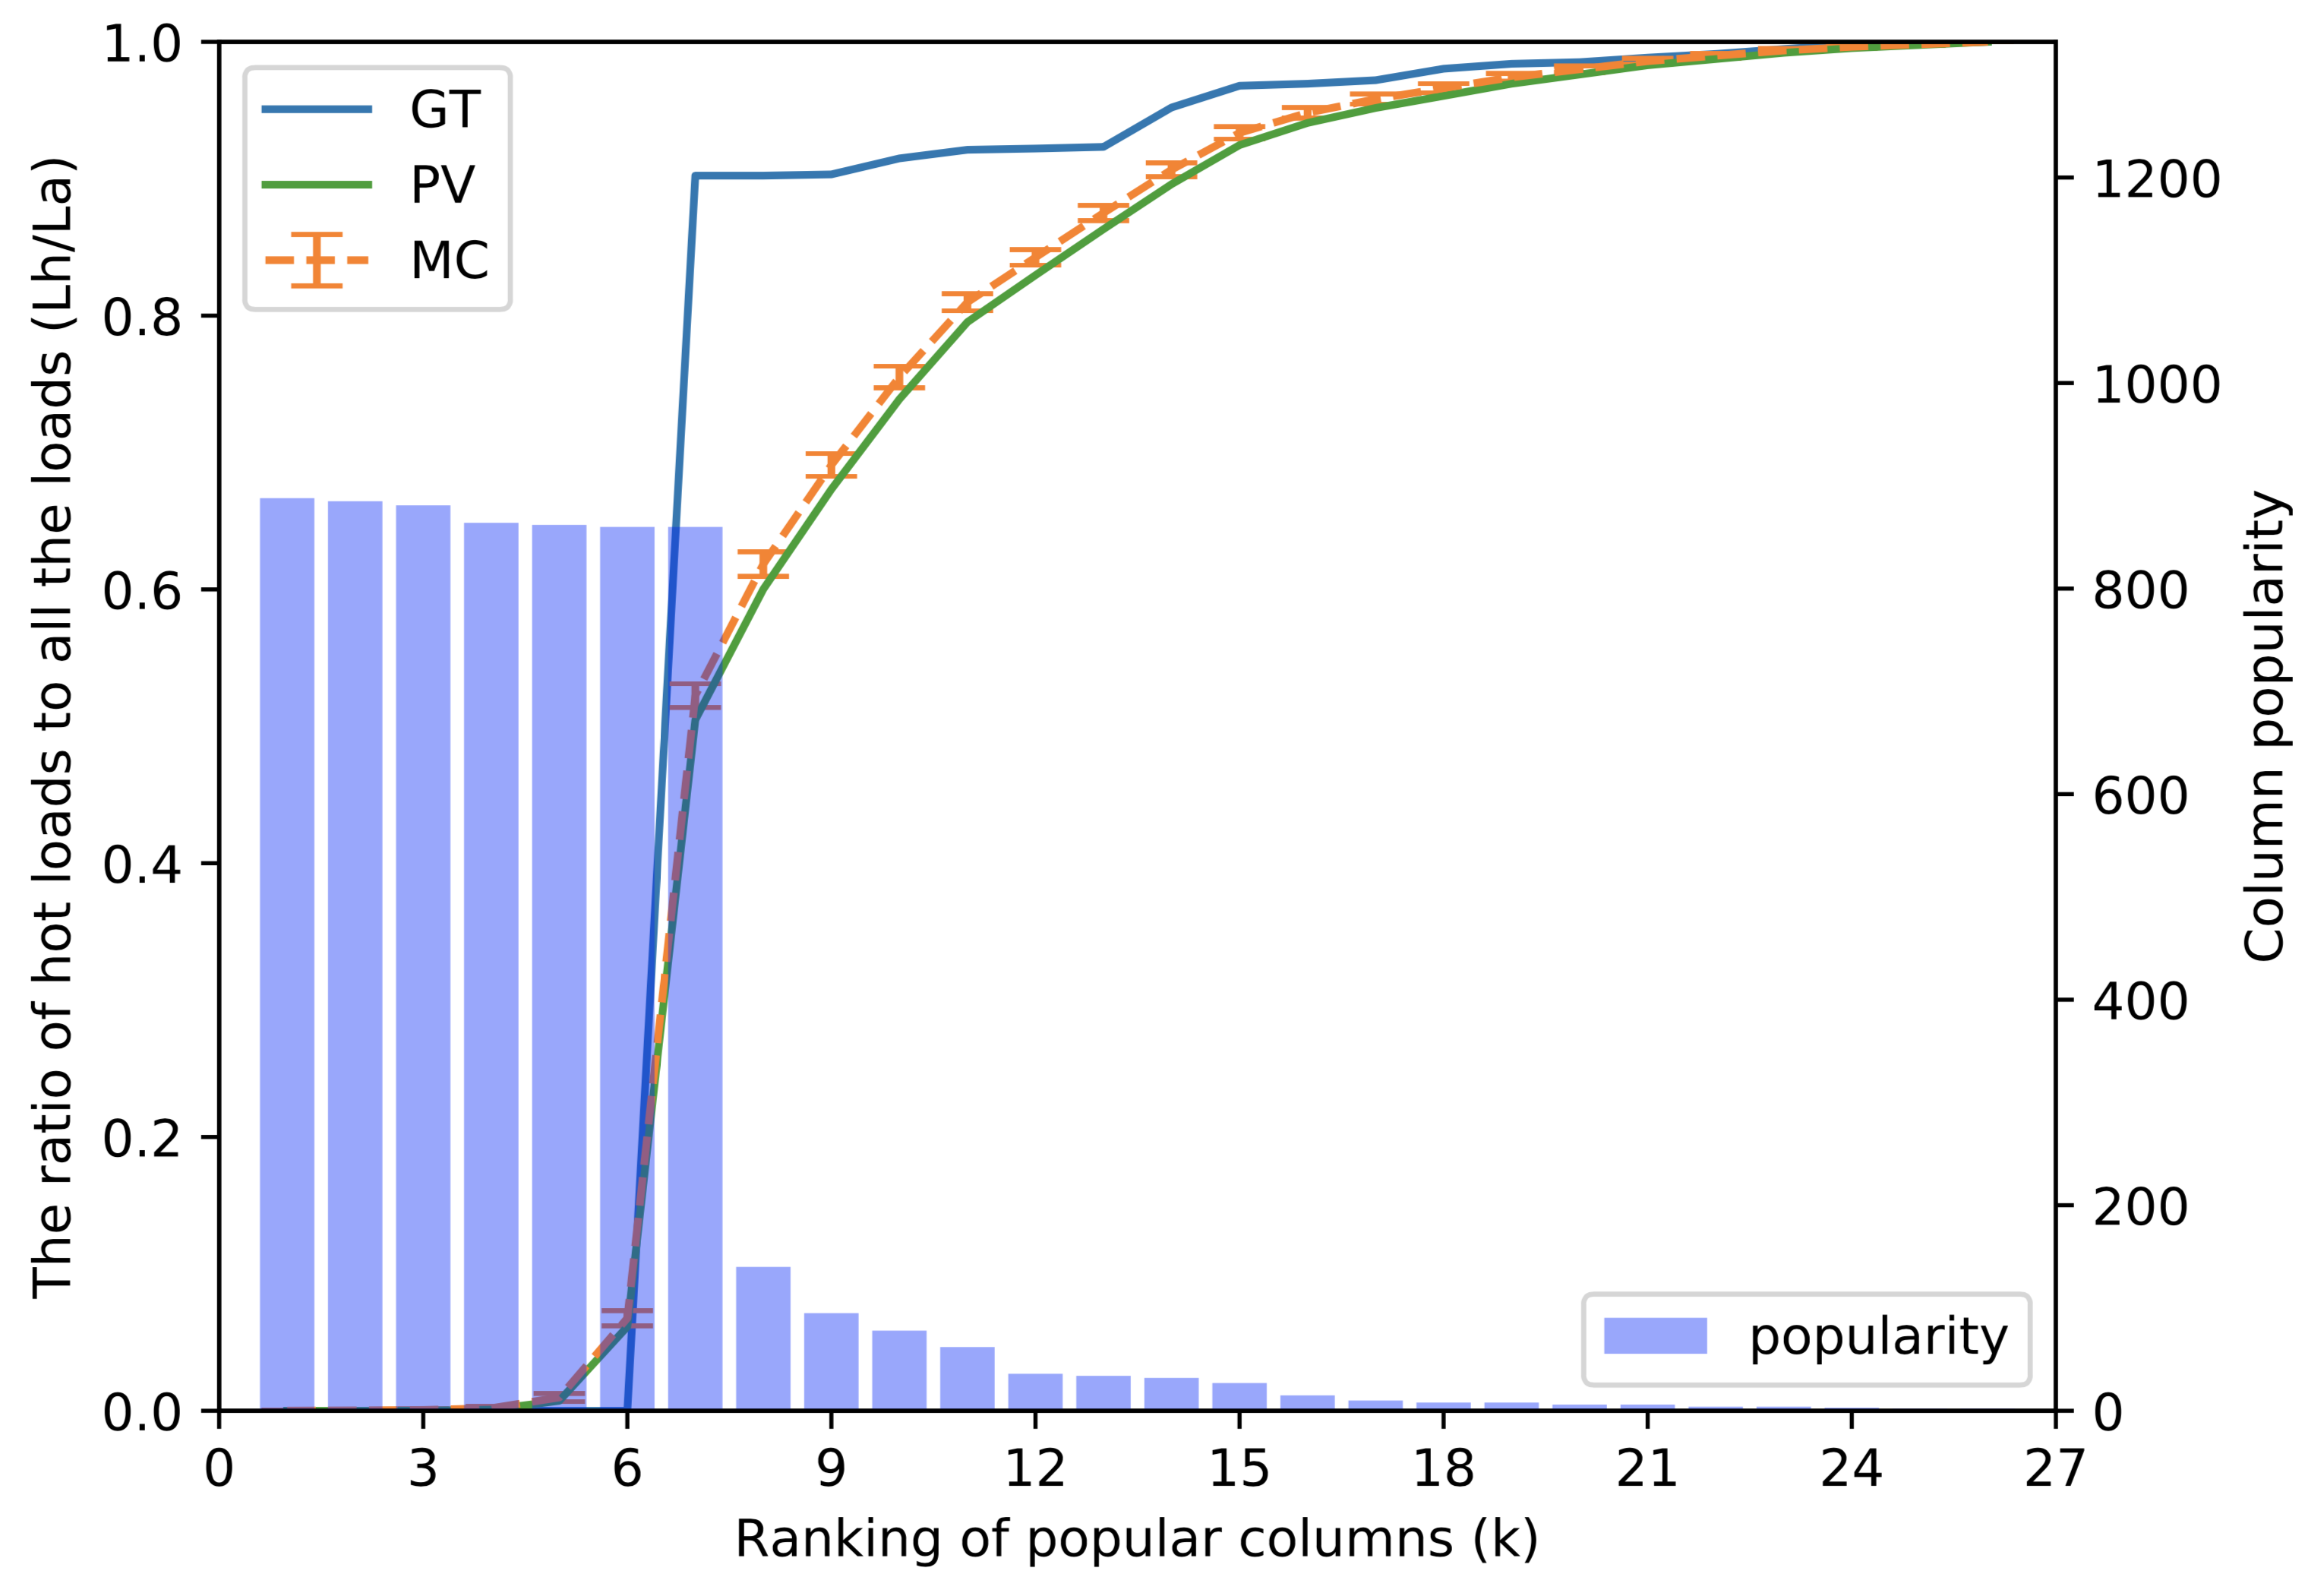
\includegraphics[width=1\textwidth]{img/cw-cache/emul_web_sales}
            \caption{TPC-DS中的 $web\_sales$ 表。}
            \label{fig:emul-ws}
        \end{subfigure}%
        \caption{负载差异大(skewed workloads)的情况下,蒙特卡罗方法、实际值和公式预测值的比较。}
        \label{fig:mc_pv_gt}
        %\vspace{-.1in}
    \end{minipage}
\end{figure}


\par \noindent\textbf{测量实验3} 我们加入了更多测试来验证$L_h$ 和 $k$之间的关系,其中用到的负载热度差异更大。具体来说,不同于之前对TPC-DS标准测试程序提供的查询任务只计数一次,我们对查询任务的热度(数量)进行了配置,使其服从Zipf分布(指数参数设置为2)。这样一来,1) 不同列的热门度差异更大,2) 查询任务的数量更多。图~\ref{fig:mc_pv_gt} 展示了先前提到的3个例子中归一化的$L_h$ 和 $k$之间的关系。根据图中结果,我们发现 1) 因为大部分查询任务只访问很少一部分非常热门的列,大部分的负载可由复制的仅含少部分热门的列的副本承担; 2) 当查询任务的数量增加,通过等式~\ref{equ:lh}预测的$L_h$的值更加接近蒙特卡罗方法得出的值,也就更加接近实际值。


\par 总而言之,经过我们的评估,基于列的热度生成查询任务来估计访问模式的分布是可行的。此外,在列热度分布更加不均衡的情况下进行的测量实验(测量实验3)也启发我们,把前$k$个最热门的列“捆绑”复制是有利的。

数据Shuffling与数据放置的位置、网络通信状况、任务调度等因素均有关,非常复杂,它产生的影响难以进行确定性的数学建模进行研究
\par 在本章我们会对我们的目标问题进行数学建模,


\chapter{实现}
\label{chp:implementation}
\chapter{测试与评估}


\chapter{总结与展望}
\label{chp:future}


数据Shuffling与数据放置的位置、网络通信状况、任务调度等因素均有关,非常复杂,它产生的影响难以进行确定性的数学建模进行研究

\end{Main} % 结束正文


% 参考文献
\bibliography{seuthesis}

\begin{Appendix}

\chapter{Bundle-K方案核心代码}
\label{appendix:bundle-k-code}

\begin{lstlisting}[language=java]

package alluxio.master.repl.policy;

import alluxio.Configuration;
import alluxio.PropertyKey;
import alluxio.collections.Pair;
import alluxio.master.block.BlockMasterFactory;
import alluxio.master.repl.meta.FileAccessInfo;
import fr.client.utils.MultiReplUnit;
import fr.client.utils.OffLenPair;
import fr.client.utils.ReplUnit;
import org.slf4j.Logger;
import org.slf4j.LoggerFactory;

import java.util.Collections;
import java.util.List;
import java.util.stream.Collectors;

/**
*
*/
public class BundleHottestKPolicy implements ReplPolicy {
    private static final Logger LOG = LoggerFactory.getLogger(BundleHottestKPolicy.class);

    private double weight;
    private int workNum;

    public BundleHottestKPolicy() {
        weight = Configuration.getDouble(PropertyKey.FR_REPL_WEIGHT);
    }

    private void updateWorkNum(){
        workNum = BlockMasterFactory.getBlockMaster().getWorkerCount();
    }

    private double calcObjective(double hotLoad, double coldLoad, double hotSize, int r){
        double hotSqu = hotLoad * hotLoad;
        double coldSqu = coldLoad * coldLoad;

        return (hotSqu / r + coldSqu) / workNum - (hotSqu + coldSqu) / (workNum * workNum) + weight * r * hotSize;
    }

    @Override
    public List<ReplUnit> calcReplicas(FileAccessInfo fileAccessInfo) {
        updateWorkNum();

        List<Pair<OffLenPair, Long>> allPops = fileAccessInfo
                .getOffsetCount()
                .entrySet()
                .stream()
                .map( o -> new Pair<>(o.getKey(), o.getValue()))
                .collect(Collectors.toList());

        long totalSize = allPops
                .stream()
                .mapToLong(o -> o.getFirst().length)
                .reduce((long) 0, Long::sum);

        List<Pair<OffLenPair, Double>> sortedLoads = allPops
                .stream()
                .map( o -> new Pair<>(o.getFirst(), o.getFirst().length * o.getSecond() * 1.0 / totalSize))
                .sorted((e1, e2) -> e1.getSecond() < e2.getSecond()?1:-1)
                .collect(Collectors.toList());

        LOG.info("file: {}. sorted loads: {}", fileAccessInfo.getFilePath().getPath(), sortedLoads);


        List<Pair<OffLenPair, Long>> sortedPops = sortedLoads
                .stream()
                .map( o -> new Pair<>(o.getFirst(), fileAccessInfo.getOffsetCount().get(o.getFirst())))
                .collect(Collectors.toList());

        LOG.info("query_num: {}. sorted pops: {}", fileAccessInfo.getQueryNum(), sortedPops);

        List<Double> sortedSizes = sortedPops
                .stream()
                .map( o -> o.getFirst().length * 1.0 / totalSize)
                .collect(Collectors.toList());

        double allLoad = sortedLoads.stream().mapToDouble(Pair::getSecond).reduce(0.0, Double::sum);

        int bestK = -1;
        int bestR = -1;
        // initial obj as no replicas
//        double bestObj = calcObjective(0, allLoad, 0, 0);
        double bestObj = Double.POSITIVE_INFINITY;

        for(int k = 0; k < sortedPops.size(); k++){

            double hotLoad = sortedLoads
                    .stream()
                    .limit(k + 1)
                    .mapToDouble(Pair::getSecond)
                    .reduce( 0.0, Double::sum);

            double regret = sortedPops
                    .stream()
                    .skip(k + 1)
                    .mapToDouble( o -> 1 - o.getSecond() * 1.0 / fileAccessInfo.getQueryNum())
                    .reduce(1.0, (d1, d2) -> d1 * d2);

            hotLoad = hotLoad * regret;

            double coldLoad = allLoad - hotLoad;

            double hotSize = sortedSizes
                    .stream()
                    .limit(k + 1)
                    .reduce(0.0, Double::sum);

            double doubleR = Math.sqrt(hotLoad * hotLoad / (workNum * weight * hotSize));

//            System.out.println("k=" + k + "; Lh=" + hotLoad + "; workNum=" + workNum + "; Sh=" + hotSize + "; r=" + doubleR);

            if (doubleR > workNum){
                double localObj = calcObjective(hotLoad, coldLoad, hotSize, workNum);
                if (localObj < bestObj){
                    bestObj = localObj;
                    bestK = k;
                    bestR = workNum;
                }
            }
            else {
                int floorR = (int) Math.floor(doubleR);
                int ceilR = (int) Math.ceil(doubleR);

                double floorObj = calcObjective(hotLoad, coldLoad, hotSize, floorR);
                double ceilObj = calcObjective(hotLoad, coldLoad, hotSize, ceilR);

                double localObj = Math.min(floorObj, ceilObj);
                if (localObj < bestObj){
                    bestObj = localObj;
                    bestK = k;
                    bestR = floorObj < ceilObj ? floorR : ceilR;
                }
            }

        }

        LOG.info("Opt K = {}; Opt R = {}; Opt Obj = {}", bestK, bestR, bestObj);

        List<OffLenPair> replPairs = sortedPops
                .stream()
                .limit(bestK + 1)
                .map(Pair::getFirst)
                .collect(Collectors.toList());

        return Collections.singletonList(new ReplUnit(replPairs, bestR));
    }

    @Override
    public List<MultiReplUnit> calcMultiReplicas(List<FileAccessInfo> fileAccessInfos) {
        return null;
    }
}
    

\end{lstlisting}







\end{Appendix}

\begin{Acknowledgement}{}
    这次的毕业论文设计总结是在我的指导老师xxx老师亲切关怀和悉心指导下完成的。从毕业设计选题到设计完成,x老师给予了我耐心指导与细心关怀,有了莫老师耐心指导与细心关怀我才不会在设计的过程中迷失方向,失去前进动力。x老师有严肃的科学态度,严谨的治学精神和精益求精的工作作风,这些都是我所需要学习的,感谢x老师给予了我这样一个学习机会,谢谢!
    
      感谢与我并肩作战的舍友与同学们,感谢关心我支持我的朋友们,感谢学校领导、老师们,感谢你们给予我的帮助与关怀;感谢肇庆学院,特别感谢计算机科学与软件学院四年来为我提供的良好学习环境,谢谢!
\end{Acknowledgement}

\newpage
\printindex % 索引

%\begin{thebibliography}{99}


%\bibliographystyle{ieee}
%\bibliography{seuthesis}


\end{document}
